\documentclass[12pt,openright,twoside,a4paper,english,french,spanish]{abntex2}

\usepackage{cmap}	
\usepackage{lmodern}	
\usepackage[T1]{fontenc}	
\usepackage[utf8]{inputenc}		
\usepackage{lastpage}		
\usepackage{indentfirst}
\usepackage{color}	
\usepackage{graphicx}	
\usepackage{units}
\usepackage[brazilian,hyperpageref]{backref}
\usepackage[alf]{abntex2cite}
\usepackage{bold-extra}
\usepackage{eso-pic}
\usepackage{listings}
\usepackage[table,xcdraw]{xcolor}
\usepackage{caption}
\usepackage{multicol}
\usepackage{tcolorbox}
\usepackage{amsmath}

%Using tikz for diagrams, sankey, venn, etc

\usepackage{tikz}
\usetikzlibrary{shapes,arrows,fit,positioning}
\usepackage{longtable}
\usepackage{makeidx}
%\usepackage{hyperref}

\renewcommand{\backrefpagesname}{Citado na(s) página(s):~}
\renewcommand{\backref}{}
\renewcommand*{\backrefalt}[4]{
	\ifcase #1 %
		Nenhuma citação no texto.%
	\or
		Citado na página #2.%
	\else
		Citado #1 vezes nas páginas #2.%
	\fi}%
% ---

	\renewcommand{\lstlistlistingname}{Lista de Códigos}

\newcommand{\addtoindex}[1]{#1\index{#1}}
\newcommand{\curso}[1]{\def\imprimircurso{#1}}

\newcommand{\palavraChaveUm}[1]{\def\imprimirpalavrachaveum{#1}}
\newcommand{\palavraChaveDois}[1]{\def\imprimirpalavrachavedois{#1}}

\newcommand{\cdu}[1]{\def\nomecdu{#1}}
\newcommand{\dataDaAprovacao}[1]{\def\imprimirdatadaaprovacao{#1}}

\newcommand{\membroConvidadoUm}[1]{\def\imprimirmembroconvidadoum{#1}}
\newcommand{\membroConvidadoDois}[1]{\def\imprimirmembroconvidadodois{#1}}

\newcommand\BackgroundPic{%
	\put(0,0){%
		\parbox[b][\paperheight]{\paperwidth}{%
			\vfill
			\centering
			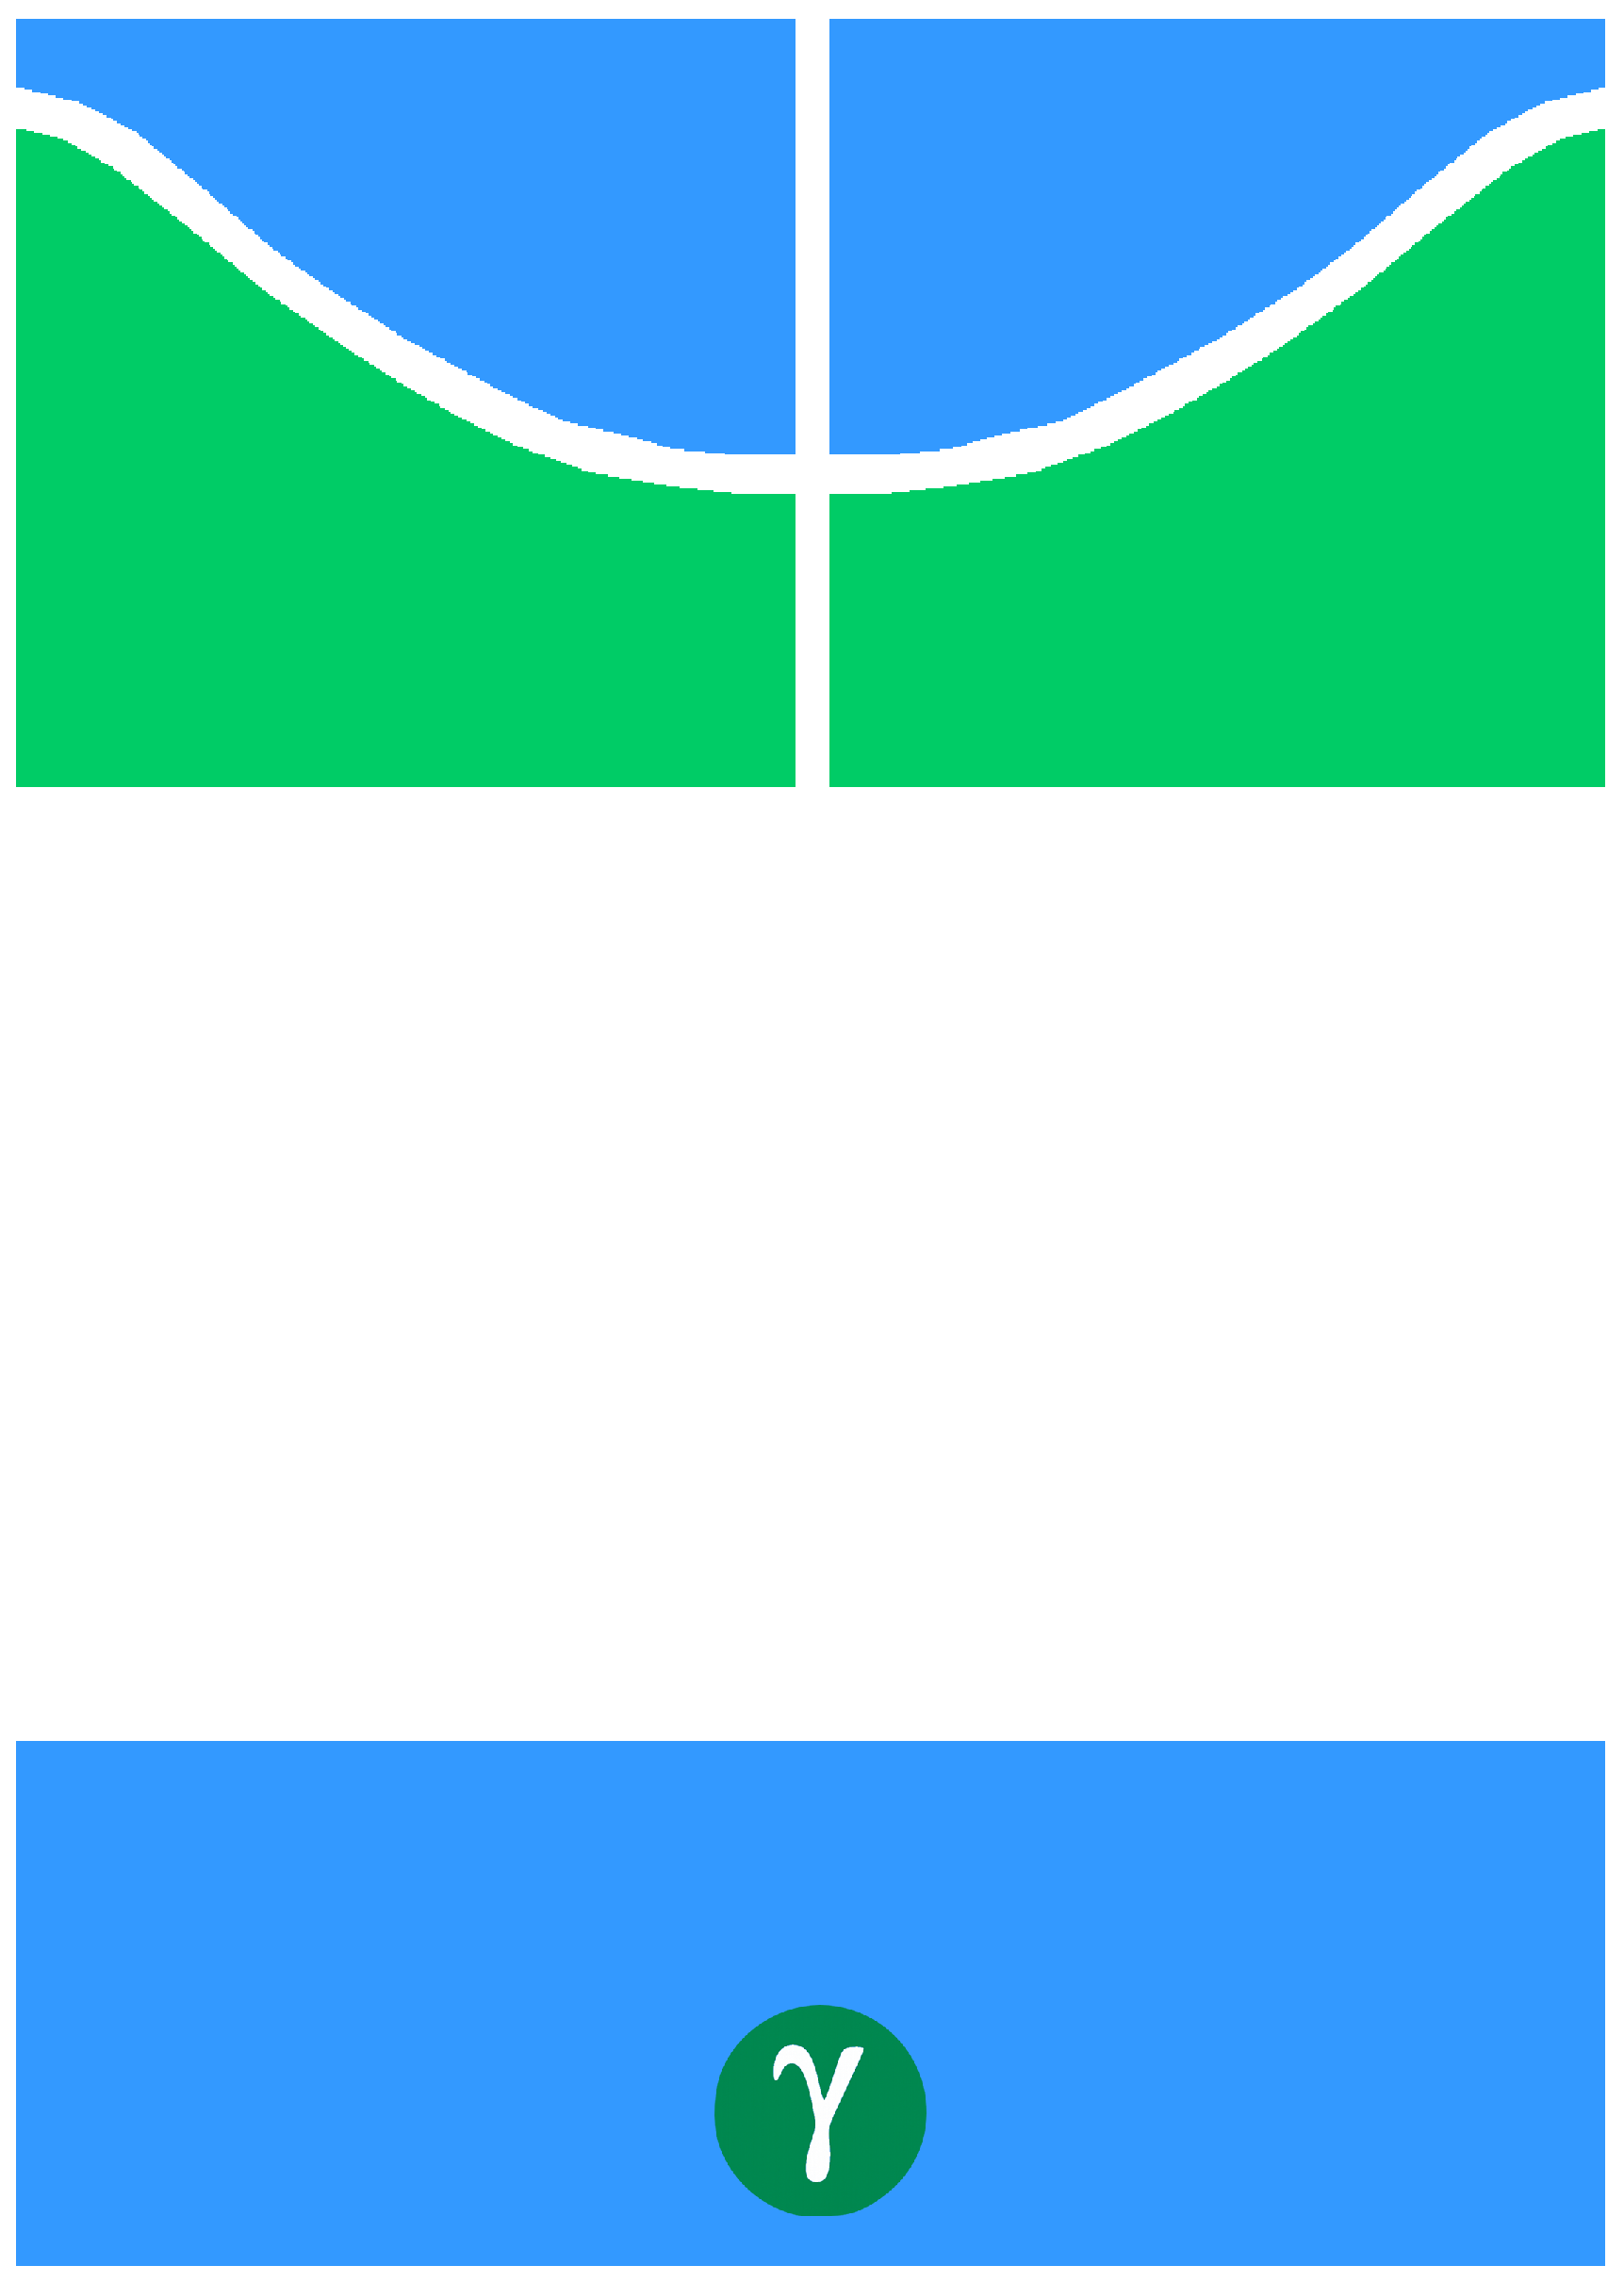
\includegraphics[width=\paperwidth,height=\paperheight,%
				keepaspectratio]{figuras/capa.eps}%
			\vfill
		}
	}
}

\renewcommand{\imprimircapa}{%
  \begin{capa}%
    \center
	\AddToShipoutPicture*{\BackgroundPic}

%	\begin{huge}
%		\textbf{\textsc{Trabalho de Conclusão de Curso}}
%	\end{huge}

    \vspace*{2.7in}
	{\textbf{\large\imprimirinstituicao}}
	\par
	{\textbf{\large\imprimircurso}}

	\vspace{0.5in}

    {\ABNTEXchapterfont\bfseries\LARGE\imprimirtitulo}
    \vspace*{\fill}
    
	\begin{flushright}
    	\textbf{{\large{Autor: \imprimirautor}}}
		\par
    	\textbf{{\large{Orientador: \imprimirorientador}}}
	\end{flushright}
		
    \vspace*{0.2in}
    \textbf{{\large\imprimirlocal}}
    \par
    \textbf{{\large\imprimirdata}}
    
    \vspace*{2.2in}
  \end{capa}
}



% Dados pessoais
\autor{Athos Ribeiro}
\curso{Engenharia de Software}

% Dados do trabalho
\titulo{Análise Estática de Código-Fonte com Foco em Segurança: Metodologia
Para Avaliação de Ferramentas}
\data{2015}
\palavraChaveUm{Análise estática, Segurança}
\palavraChaveDois{Código fonte, Vulnerabilidade}

% Dados da orientacao
\orientador{Prof. Dr. Edson Alves da Costa Júnior}
%\coorientador{(quando houver, Titulação Acadêmica e Nome do Orientador)}

% Dados para a ficha catalográfica
\cdu{02:141:005.6}

% Dados da aprovação do trabalho
\dataDaAprovacao{15 de Julho de 2015}
\membroConvidadoUm{Prof. Dr. Paulo Roberto Miranda Meirelles}
\membroConvidadoDois{Prof. Dr. Luiz Augusto Laranjeira}

\local{Brasília, DF}
\instituicao{%
  Universidade de Brasília - UnB
  \par
  Faculdade UnB Gama - FGA
}
\tipotrabalho{Trabalho de Conclusão de Curso}
\preambulo{Monografia submetida ao curso de graduação em (\imprimircurso) 
da Universidade de Brasília, como requisito parcial para obtenção do Título 
de Bacharel em (\imprimircurso).}

\definecolor{blue}{RGB}{41,5,195}
\makeatletter
\hypersetup{
     	%pagebackref=true,
		pdftitle={\@title}, 
		pdfauthor={\@author},
    	pdfsubject={\imprimirpreambulo},
	    pdfcreator={LaTeX with abnTeX2},
		pdfkeywords={abnt}{latex}{abntex}{abntex2}{trabalho acadêmico}, 
		colorlinks=true,       		% false: boxed links; true: colored links
    	linkcolor=blue,          	% color of internal links
    	citecolor=blue,        		% color of links to bibliography
    	filecolor=magenta,      		% color of file links
		urlcolor=blue,
		bookmarksdepth=4
}
\makeatother
\setlength{\parindent}{1.3cm}
\setlength{\parskip}{0.2cm}  
\makeindex

\newlistof{lstlistoflistings}{lol}{\lstlistingname}

%--------------------------------------------
%Definições para código com fundo listrado
\newcommand\realnumberstyle[1]{#1}
\makeatletter
\newcommand{\zebra}[3]{%
    {\realnumberstyle{#3}}%
    \begingroup
    \lst@basicstyle
    \ifodd\value{lstnumber}%
        \color{#1}%
    \else
        \color{#2}%
    \fi
        \rlap{
        \color@block{0.94\textwidth}{\ht\strutbox}{\dp\strutbox}%
        \hspace*{\lst@numbersep}%
        }%
    \endgroup
}
\makeatother
\renewcommand\lstlistingname{Código}

\DeclareCaptionFormat{listing}{\vskip1pt\rule{\dimexpr\textwidth\relax}{0.4pt}\par\vskip1pt{\centering#1#2#3}}
\captionsetup[lstlisting]{format=listing,singlelinecheck=false, margin=0pt, font={sf},labelsep=space,labelfont=bf}

\DeclareMathVersion{sans}
\SetSymbolFont{operators}{sans}{OT1}{cmbr}{m}{n}
\SetSymbolFont{letters}  {sans}{OML}{cmbrm}{m}{it}
\SetSymbolFont{symbols}  {sans}{OMS}{cmbrs}{m}{n}

\lstnewenvironment{sflisting}[1][]
  {\lstset{#1}\mathversion{sans}}{}

\lstset{%
language=C++,           %linguagem
numbers=left,           %posição dos números
stepnumber=1,           %frequencia de aparição dos números
numbersep=5pt,
numberstyle=\tiny\zebra{gray!15}{white!35},
basewidth={0.6em,0.45em},
fontadjust=true,
mathescape=true,
tabsize=4,
commentstyle=\color{blue},
literate={á}{{\'a}}1 {à}{{\`a}}1 {ã}{{\~a}}1 {é}{{\'e}}1 {É}{{\'E}}1 {ê}{{\^e}}1 {õ}{{\~o}}1 {í}{{\'i}}1 {ó}{{\'o}}1 {ú}{{\'u}}1 {ç}{{\c c}}1 {³}{{$^3$}}1 {Ω}{{$\Omega$}}1,
breaklines=true,
showstringspaces=false,
stringstyle=\color{cyan},
basicstyle=\footnotesize\ttfamily}



\makeindex
\begin{document}
\lstset{linewidth=15cm}

\frenchspacing 
\imprimircapa
\imprimirfolhaderosto*

\begin{fichacatalografica}
	\vspace*{\fill}					% Posição vertical
	\hrule							% Linha horizontal
	\begin{center}					% Minipage Centralizado
	\begin{minipage}[c]{12.5cm}		% Largura
	
	\imprimirautor
	
	\hspace{0.5cm} \imprimirtitulo  / \imprimirautor. --
	\imprimirlocal, \imprimirdata-
	
	\hspace{0.5cm} \pageref{LastPage} p. : il. (algumas color.) ; 30 cm.\\
	
	\hspace{0.5cm} \imprimirorientadorRotulo~\imprimirorientador\\
	
	\hspace{0.5cm}
	\parbox[t]{\textwidth}{\imprimirtipotrabalho~--~\imprimirinstituicao,
	\imprimirdata.}\\
	
	\hspace{0.5cm}
		1. \imprimirpalavrachaveum.
		2. \imprimirpalavrachavedois.
		I. \imprimirorientador.
		II. Universidade de Brasília.
		III. Faculdade UnB Gama.
		IV. \imprimirtitulo\\ 			
	
	\hspace{8.75cm} CDU \nomecdu\\
	
	\end{minipage}
	\end{center}
	\hrule
\end{fichacatalografica}

%\begin{errata}
Elemento opcional da \citeonline[4.2.1.2]{NBR14724:2011}. \textbf{Caso não 
deseje uma errata, deixar todo este arquivo em branco}. Exemplo:

\vspace{\onelineskip}

FERRIGNO, C. R. A. \textbf{Tratamento de neoplasias ósseas apendiculares com
reimplantação de enxerto ósseo autólogo autoclavado associado ao plasma
rico em plaquetas}: estudo crítico na cirurgia de preservação de membro em
cães. 2011. 128 f. Tese (Livre-Docência) - Faculdade de Medicina Veterinária e
Zootecnia, Universidade de São Paulo, São Paulo, 2011.

\begin{table}[htb]
\center
\footnotesize
\begin{tabular}{|p{1.4cm}|p{1cm}|p{3cm}|p{3cm}|}
  \hline
   \textbf{Folha} & \textbf{Linha}  & \textbf{Onde se lê}  & \textbf{Leia-se}  \\
    \hline
    1 & 10 & auto-conclavo & autoconclavo\\
   \hline
\end{tabular}
\end{table}

\end{errata}

\begin{folhadeaprovacao}

  \begin{center}
    {\ABNTEXchapterfont\large\imprimirautor}

    \vspace*{\fill}\vspace*{\fill}
    {\ABNTEXchapterfont\bfseries\Large\imprimirtitulo}
    \vspace*{\fill}
    
    \hspace{.45\textwidth}
    \begin{minipage}{.5\textwidth}
        \imprimirpreambulo
    \end{minipage}%
    \vspace*{\fill}
   \end{center}
    
   Trabalho aprovado. \imprimirlocal, \imprimirdatadaaprovacao:

   \assinatura{\textbf{\imprimirorientador} \\ Orientador} 
   \assinatura{\textbf{\imprimirmembroconvidadoum} \\ Convidado 1}
   \assinatura{\textbf{\imprimirmembroconvidadodois} \\ Convidado 2}
      
   \begin{center}
    \vspace*{0.5cm}
    {\large\imprimirlocal}
    \par
    {\large\imprimirdata}
    \vspace*{1cm}
  \end{center}
  
\end{folhadeaprovacao}

%\begin{dedicatoria}
   \vspace*{\fill}
   \centering
   \noindent
	\textbf{A dedicatória é opcional. Caso não deseje uma, deixar todo este
	arquivo em branco}.

   \textit{Este trabalho é dedicado às crianças adultas que,\\
   quando pequenas, sonharam em se tornar cientistas.} \vspace*{\fill}
\end{dedicatoria}

%\begin{agradecimentos}
Agradeço ao meu orientador, professor Dr. Edson Alves, por sua dedicação à Universidade de Brasília, especialmente à FGA e por inspirar seus alunos, que como eu, tanto admiram seu trabalho. Ao professor Dr. Luiz Augusto Laranjeira, pela oportunidade que me foi dada de conhecer e trabalhar no National Institute of Standards and Technology, conduzindo as pesquisas que inspiraram a realização deste trabalho. Ao Dr. Paul E. Black pela paciência e ensinamentos que me foram passados ao longo da minha estadia no NIST em 2014 e a toda a equipe do Software Assurance Metrics And Tool Evaluation, por me receberem tão bem, mesmo que por um curto período, como membro da sua equipe de trabalho. À toda equipe do Laboratório Avançado de Produção Pesquisa e Inovação em Software da UnB, por tudo que me foi ensinado e pela ótima relação construída ao longo dos anos, dentro e fora do laboratório. Ao professor Dr. Paulo Meirelles, pois é através da confiança que nos é depositada que nos tornamos pessoas melhores todos os dias. Por fim, agradeço aos meus pais, Edivaldo e Rita, pelo apoio incondicional.
%A inclusão desta seção de agradecimentos é opcional, portanto, sua inclusão 
%fica a critério do(s) autor(es), que caso deseje(em) fazê-lo deverá(ão) 
%utilizar este espaço, seguindo a formatação de \textit{espaço simples e 
%fonte padrão do texto (arial ou times, tamanho 12 sem negritos, aspas ou 
%itálico}.

\end{agradecimentos}

%\begin{epigrafe}
    \vspace*{\fill}
	\begin{flushright}

		\textit{``Um homem munido de papel, lápis e borracha, \\
		e submetido a uma disciplina rigorosa é, \\
		para todos os efeitos, uma máquina universal.'' \\
		(Alan Turing)}
	\end{flushright}
\end{epigrafe}

\begin{resumo}

Uma das técnicas para se reduzir o número de vulnerabilidades presentes em
software é através da detecção e resolução de defeitos presentes no código fonte
do mesmo. A detecção de tais defeitos pode ser automatizada com ferramentas de
análise estática de código fonte, quando estas têm um foco em aspectos de
segurança. O presente trabalho apresenta uma metodologia para que se avaliem
ferramentas de análise estática de código fonte com foco em segurança, desde a
seleção das ferramentas a serem avaliadas à apresentação dos resultados da
avaliação. Por fim, o trabalho apresenta exemplos de uso da metodologia
apresentada, onde se avaliam a capacidade de detecção de loops infinitos por
algumas ferramentas Livres e a corretude da análise de uma ferramenta que se
propõe a realizar análises corretas. 

 \vspace{\onelineskip}
    
 \noindent
 \textbf{Palavras-chaves}: Análise estática; Segurança; Código fonte; Vulnerabilidade.
\end{resumo}

\begin{resumo}[Abstract]
 \begin{otherlanguage*}{english}

   One technique to reduce the number of vulnerabilities found in software is
   the detection and resolution of flaws present in the source code.
   The detection of these flaws may be automated with static analysis tools,
   when these tools focus the security aspects of the source code. This work
   presents an approach to evaluate static analysis tools with focus in
   security, since the selection of the tools being evaluated to the
   presentation of the evaluation results. Later, it presents usage examples
   for the proposed approach, the ability of some Free (as in freedom) static
   analyzers to detect infinite loops and the soundess of the analysis of a tool
   that claims to be sound are evaluated. 

   \vspace{\onelineskip}
 
   \noindent 
   \textbf{Key-words}: static analysis; security; source code; vulnerability.
 \end{otherlanguage*}
\end{resumo}

\pdfbookmark[0]{\listfigurename}{lof}
\listoffigures*
\cleardoublepage
%\pdfbookmark[0]{\listtablename}{lot}
%\listoftables*
%\cleardoublepage
\renewcommand\lstlistingname{Lista de Códigos}
%\pdfbookmark[0]{\lstlistingname}{lot}
\lstlistoflistings
\cleardoublepage

\begin{siglas}
  \item[CAS] Center for Assured Software - Centro Para Software Garantido
  \item[CEA] Commissariat à l'énergie atomique et aux énergies alternatives - Comissão de Energia Atômica e Energias Alternativas
  \item[CSV] Comma Separated Value - Valor Separado por Vírgula
  \item[CVE] Common Vulnerabilities and Exposures - Vulnerabilidades e Exposições Comuns
  \item[CWE] Common Weakness Enumeration - Enumeração de Fraquezas Comum
  \item[DHS] Department of Homeland Security - Departamento de Segurança Nacional
  \item[GCC] GNU Compiler Collection - Coleção de compilador GNU
  \item[GNU] GNU's Not UNIX - GNU Não é UNIX
  \item[GPL] GNU General Public License - Licença Pública Geral
  \item[IARPA] Intelligence Advanced Research Projects Activity - Atividade de Projetos de Pesquisa Avançada de Inteligência
  \item[LGPL] Lesser General Public License - Licença Pública Geral Menor
  \item[NIST] National Institute of Standards and Technology - Instituto Nacional de Padrões e Tecnologia
  \item[NSA] National Security Agency - Agência de Segurança Nacional
  \item[NVD] National Vulnerability Database - Base de Dados de Vulnerabilidades Nacional
  \item[SAMATE] Software Assurance Metrics And Tool Evaluation - Avaliação de Métricas e Ferramentas de Garantia de Software
  \item[SARD] Software Assurance Reference Dataset - Conjunto de Dados de Referência de Garantia de Software
  \item[SATE] Static Analysis Tool Exposition - Exposição de Ferramentas de Análise Estática
  \item[SQL] Structure Query Language - Linguagem de Consulta Estruturada
  \item[SRD] SAMATE Reference Dataset - Conjunto de Dados do SAMATE
  \item[STONESOUP] Securely Taking On New Executable Software of Uncertain Provenance - Recebendo Software Executável de Proveniência Incerta de Forma Segura
  \item[SWAMP] Software Assurance Marketplace - Mercado de Garantia de Software
  \item[XML] eXtensible Markup Language - Linguagem de Marcação Extensível
  \item[YAML] YAML Ain't Markup Language - YAML Não é Linguagem de Marcação
\end{siglas}

%\begin{simbolos}
  \item[$ \Gamma $] Letra grega Gama
  \item[$ \Lambda $] Lambda
  \item[$ \zeta $] Letra grega minúscula zeta
  \item[$ \in $] Pertence
\end{simbolos}

\pdfbookmark[0]{\contentsname}{toc}
\tableofcontents*
\cleardoublepage


\textual

\chapter{Introdução} \label{introducao}

\section{Contextualização do problema}

Em plena era da informação, vivemos em uma sociedade altamente dependente de computadores \cite{inclusao}, aos quais utilizamos de forma direta ou indireta todos os dias: pagamos contas, utilizamos redes elétricas e de telefonia e sistemas de transporte como metrôs.  Falhas de software podem causar perdas irreparáveis, como roubo em massa de números de cartões de crédito\footnote{\url{http://www.theguardian.com/technology/blog/2011/apr/29/playstation-network-hackers-credit-cards}}, acidentes nucleares \cite{stuxnet} e perda em massa da privacidade dos cidadãos \cite{snowden}.

Apenas em 2014, foram registradas 7.937 vulnerabilidades no NVD (National Vulnerability Database)\footnote{\url{https://web.nvd.nist.gov/view/vuln/statistics-results?adv_search=true&cves=on}}, um banco de dados mantido pelo NIST (National Institute of Standards and Technology) que mantém registro de todas as vulnerabilidades de software publicamente conhecidas pela indústria e academia. Este foi o maior número de vulnerabilidades registrado em um único ano pelo NVD. Dentre as vulnerabilidades registradas estão o \textit{shellshock}\footnote{\url{https://cve.mitre.org/cgi-bin/cvename.cgi?name=CVE-2014-6271}} e o \textit{heartbleed} \cite{heartbleed}, duas das vulnerabilidades mais críticas já publicadas \cite{heartbleed}.

Dada a dependência da sociedade aos software que a tangem e o crescente número de vulnerabilidades encontradas nos mesmos, passa-se a buscar técnicas e métodos para aumentar a segurança de software \cite{sociedade}.

Embora acredite-se que buscar a melhoria da garantia de qualidade não seja suficiente para aumentar a segurança do software, segurança de software e qualidade de código estão fortemente relacionadas \cite{secure_programming}.

\section{Hipótese}

Avaliar ferramentas de análise estática de código não é uma tarefa simples.
Inicialmente deve-se ter um escopo bem definido, como em \cite{harvard}, onde o autor propõe metodologia específica para a seleção de ferramentas de análise estática para a detecção de defeitos relacionados a \textit{Buffer Overflows}, dado que análise estática pode ser utilizada para contextos variados e específicos, como aquisição de métricas de qualidade como apresentado por \cite{meirelles2013} e \cite{analizoartigo}, estilo, defeitos relacionados à segurança, ou qualquer outro tipo de informação sobre o código que o desenvolvedor da ferramenta acreditar ser relevante.

Para \cite{secure_programming}, a ferramenta de análise estática pode se especializar em encontrar defeitos específicos ou o máximo de defeitos que seu nível de maturidade e técnicas de análise lhe permitirem encontrar. Além disso, os desenvolvedores da ferramenta podem optar por análises completas, corretas ou nenhuma das abordagens, buscando minimizar a quantidade de falsos positivos e falsos negativos gerados pela análise. Todos os fatores mencionados devem ser considerados no momento da seleção de ferramentas de análise estática de código fonte, sendo assim, este trabalho busca apresentar uma metodologia bem definida que possa ser facilmente replicada para que se avaliem ferramentas de análise estática de código fonte voltadas à segurança.

Note que sempre que o termo \textit{análise estática de código-fonte} for mencionado ao longo deste trabalho, o autor se refere à análise estatica de código-fonte voltada à segurança a menos que qualquer outro fim esteja explícito junto ao termo.

\section{Objetivos}
\subsection{Objetivo Geral}

Definir metodologia replicável e de fácil compreensão para avaliação de ferramentas de análise estática de código-fonte com foco em segurança.

\subsection{Objetivos Específicos}

Analisar processos de avaliação ou seleção de ferramentas de análise estática utilizados em estudos anteriores;
Definir processo para avaliação de ferramentas de análise estática explicitando cada uma de suas atividades;
Validar o processo definido através de estudos de caso;

\section{Delimitação do escopo}

O trabalho busca propor metodologia replicável para análise estática de código-fonte, de modo que outras pessoas ou instituições, além das mencionadas em \nameref{fundamentacao_teorica} possam ter alguma base para iniciar pesquisas relacionadas à ferramentas de análise estática com foco em segurança. Este tipo de processo de avaliação deve ser melhorado ao longo de inúmeras iterações, de modo que o processo aqui apresentado trata-se de uma primeira versão do processo e não cabe à este trabalho apresentar etapas para melhoria do processo apresentado. Além disto, os estudos de caso apresentados ao final deste trabalho não visam avaliar de fato as ferramentas apresentas, visam apenas validar a metodologia proposta.

\section{Outline do trabalho}

Este trabalho foi dividido em 6 capítulos, o primeiro deles, \nameref{introducao}, contextualiza o problema a ser atacado e apresenta uma hipótese e escopo para este trabalho. Em seguida, o Capítulo \nameref{fundamentacao_teorica} define análise estática e outros termos utilizados ao longo dos outros capítulos e termina apresentando trabalhos que apresentam algum elo com avaliação de ferramentas ou análise estática de código fonte. Em \nameref{metodologia} apresentam-se as técnicas utilizadas para elaboração do trabalho e as decisões tomadas para a seleção das bibliografias relevantes para o mesmo. O Capítulo \nameref{metodologia_proposta} apresenta uma metodologia para avaliar ferramentas de análise estática com foco em segurança. Tal metodologia é uma formalização e generalização de conceitos obtidos  a partir de experiências adquiridas ao longo de 12 meses de interação com o SAMATE\footnote{\url{http://samate.nist.gov}}, seu conjunto de dados de referência para garantia de software, SARD\footnote{\url{http://samate.nist.gov/SARD/}}, e a quinta edição de seu programa de Avaliação de Ferramentas de Análise Estática, SATE V\footnote{\url{http://samate.nist.gov/SATE.html}}, bem como a participação do autor na avaliação das ferramentas em uma das categorias do SATE V\footnote{\url{http://samate.nist.gov/SATE5OckhamCriteria.html}}. Em \nameref{exemplos_de_uso}, apresentam-se 2 estudos de caso onde se aplicam a metodologia aqui proposta: um estudo de avaliação de ferramentas de licenças livres apontadas pelo NIST e uma aplicação desta metodologia para realização das avaliações referentes à Ockham Criteria. Por fim, o Capítulo \nameref{conclusoes} encerra o trabalho, avaliando a metodologia apresentada através dos resultados obtidos nos estudos de caso e apontando trabalhos futuros relacionados à mesma e à outros tópicos relevantes.

\chapter{Fundamentação teórica}\label{fundamentacao_teorica}

Este capitulo contextualiza o presente trabalho, apresentando definições de conceitos que serão utilizados em outros capítulos. Inicialmente define-se análise estática de código fonte e apresentam-se exemplos métricas para um contexto de segurança. Em seguida, são apresentadas algumas ferramentas para análise estática, bem como a definição exemplos de bases de dados de vulnerabilidades. Por fim, discutem-se trabalhos relacionados à análise estática com foco em segurança e avaliações deste tipo de ferramenta.

\section{Análise estática de código}\label{fundamentacao_teorica:analise_estatica_de_codigo}

Metade dos defeitos de segurança de software são introduzidos à nível de código-fonte \cite{vadim}. Em tal contexto, software pode ser verificado através da análise dinâmica ou da análise estática \cite{concolic}.

Técnicas de análise dinâmica são baseadas na análise de software realizada através da execução do programa analisado, em um processador real ou virtual \cite{concolic}, e podem encontrar defeitos ao longo da fase de testes. Mas para tal necessitam que o código esteja em um estado em que possa ser executado e instalado. Além disso, apenas os defeitos que se encontram no caminho de execução que as entradas dos testes fornecem podem ser encontrados \cite{harvard}.

Análise estática de código é a análise de programas de computador sem a necessidade de executar tais programas, geralmente feita por ferramentas externas, de forma automatizada \cite{kannavara}. À tais ferramentas dá-se o nome de ferramenta de análise estática de código fonte, ou simplesmente ferramenta de análise estática. Segundo \cite{secure_programming}, qualquer ferramenta que analisa código sem o executar está realizando análise estática de código.

Ferramentas de análise estática podem inferir informações  acerca de um software sem a necessidade de executar o mesmo, tornando-as ferramentas adequadas para detecção de fraquezas no código \cite{vadim}. Deste modo, tais ferramentas se mostram um ponto razoável para que se possa buscar maior qualidade final do software \cite{sa_spec}.

\textbf{Fraquezas} são defeitos de software provenientes do design, implementação ou outras áreas do ciclo de desenvolvimento do software. Em condições específicas, fraquezas podem contribuir para a introdução de \textbf{vulnerabilidades} no software. Quando ativadas, estas vulnerabilidades (manifestações de fraquezas) resultam em falhas de sistema, ou simplesmente falhas.

``Muitas vezes os termos fraqueza e vulnerabilidade são confundidos ou as pessoas discordam de suas definições. As ferramentas de análise estática buscam por fraquezas no código, quando as pessoas, em grande parte das vezes, gostariam que elas buscassem por vulnerabilidades''\footnote{por Steven M. Christey, engenheiro de segurança da informação do MITRE em uma lista de discussão sobre segurança web disponível em \url{http://lists.webappsec.org/pipermail/websecurity_lists.webappsec.org/2011-November/008118.html}}.

O MITRE é uma organização sem fins lucrativos que opera centros de pesquisa e desenvolvimento patrocinados pelo governo federal dos Estados Unidos da América. Uma das iniciativas do MITRE, patrocinada por um projeto de métricas de qualidade de software e avaliação de ferramentas (SAMATE - Software Assurance Metrics and Tool Evaluation), visa elaborar e manter um catálogo de fraquezas de software, onde as fraquezas de software conhecidas recebem uma definição formal e um número identificador. Tal catálogo de fraquezas é conhecido como Common Weakness Enumeration ou CWE\footnote{\url{cwe.mitre.org}}, e tem sido amplamente adotado para referenciar fraquezas de software, tanto na indústria quanto na academia.

Consideraremos fraquezas de software apenas os defeitos que estiverem mapeadas como fraquezas em forma de CWE. Sendo assim, chamaremos de defeito (ou \textit{bug}) as fraquezas do software.

Existem diferentes técnicas de análise estática de código-fonte, que variam desde simples análises léxicas, análises de fluxo de dados à análise de grafos de fluxo de controle. Ao apontar defeitos no código, uma ferramenta de análise estática pode ou não cometer erros, dada a natureza do defeito e a técnica de análise empregada. Algumas técnicas são menos complexas e estão mais suscetíveis a erros do que outras \cite{harvard}. Ainda assim, cada uma das técnicas de análise estática tem suas limitações \cite{pascal}, o que justifica o uso de e a busca por diferentes técnicas de análise.

Como definido em \cite{sa_spec}, chama-se \textbf{falso positivo}, ou alarme falso, um trecho de código apontado como defeituoso por uma ferramenta de análise estática que, na verdade, não se trata de um defeito, ou seja, a ferramenta cometeu um erro ao apontar um trecho de código não defeituoso como defeituoso. Chama-se \textbf{falso negativo} um defeito no código fonte, que se enquadra na categoria de defeitos detectados pela ferramenta que analisa o código em questão, que não foi detectado pela ferramenta, ou seja, a ferramenta cometeu um erro ao não apontar um trecho de código defeituoso.

Uma ferramenta ideal não cometeria erros, apontando todos os defeitos do código (mesmo que apenas em uma dada categoria) e nunca apontando um trecho de código correto como defeituoso (a ferramenta não comete falsos positivos nem falsos negativos). Trabalhos anteriores mostram que é impossível, mesmo em teoria, produzir tal ferramenta \cite{sa_spec}. É possível, porém, produzir ferramentas capazes de cometer apenas um dos erros (falsos positivos ou falsos negativos). À análise estática que não gera falsos negativos, ou seja, aponta todos os defeitos no código, chamamos \textbf{análise correta}. À análise estática que não gera falsos positivos, ou seja, todos os possíveis defeitos apontados por ela são de fato trechos de código defeituosos, chama-se \textbf{análise completa}.

\section{Métricas e métricas de segurança}

Em \cite{nsa}, o CAS (Center for Assured Software) da Agência de Segurança Nacional (NSA – National Security Agency), centro de pesquisa criado para aumentar o nível de confiança de que os software utilizados pelo Departamento de Defesa dos Estados Unidos (DoD – Department of Defense) estão livres de vulnerabilidades \cite{nsa}, apresenta um conjunto de métricas para que se aplique sua metodologia. Das métricas apresentadas, algumas são de propósito geral, ou seja, independentes da natureza da suíte de testes ou mesmo da metodologia de testes empregada na análise, desde que sejam conhecidos todos os defeitos presentes no código a ser analisado. Ao realizar seu \textit{workshop} de avaliação de ferramentas, o SATE, o NIST utiliza este conjunto de métricas descrito pelo CAS para suas análises, como notado em \cite{sate_iv}. Essas métricas são:

Positivos: Quantidade total de defeitos reportados pela ferramenta que são de fato defeitos no código-fonte analisado.

Falsos Positivos: Quantidade total de defeitos reportados pela ferramenta que não são defeitos no código-fonte analisado.

Falsos Negativos: Quantidade de defeitos presentes no código fonte que não foram reportados pela ferramenta.

Note que o conjunto que contém todos os Positivos e todos os Falsos Negativos, é o conjunto de todos os defeitos presentes no código-fonte. Tal conceito foi amplamente utilizado para as análises da Ockham Criteria\footnote{\url{http://samate.nist.gov/SATE5OckhamCriteria.html}} realizada na quinta edição do SATE\footnote{\url{http://samate.nist.gov/SATE5.html}}, pelo NIST, cujos resultados ainda não foram publicados. Chamaremos tal conjunto de Trechos Defeituosos, (Equação \eqref{eq1}),
\begin{equation}\label{eq1}
TD = P + FN,
\end{equation}
  onde $TD$ é o número de Trechos Defeituosos, $P$ o número de Positivos e $FN$ o número de Falsos Negativos.

  No contexto da Ockham Criteria do SATE V do NIST, considera-se um defeito apenas se o mesmo for uma fraqueza, ou seja, um defeito só é considerado quando formalizado de acordo com o CWE, como mencionado   na Seção \nameref{fundamentacao_teorica:analise_estatica_de_codigo} do presente trabalho. Isso implica que a Equação \eqref{eq1} pode não ser verdadeira, dado que podem existir defeitos reportados pela ferramenta que não estejam mapeados em forma de CWE, ou ainda, que estejam sujeitos à interpretação das CWE, que como mencionado em \cite{yan} e notado ao longo dos trabalhos  da Ockham Criteria, nem sempre são definidas com precisão.

  Precisão: Taxa de defeitos reportados para a quantidade total de defeitos presentes no código analisado.  Ela pode ser representada pela Equação \eqref{eq2},
\begin{equation}\label{eq2}
  P_r = \frac{P}{P + FP}
\end{equation}
  onde $P_r$ é a precisão, $P$ o número de Positivos e $FP$ o número de Falsos Positivos.

  A precisão indica a capacidade da ferramenta de identificar defeitos. Note que a precisão é indefinida quando uma ferramenta não reporta erros \cite{nsa}, pois $P = 0$, e $FP = 0$, de modo que $P_r = \frac{0}{0}$. Quando definida, $0 \leq Pr \leq 1$.

  Corretude: Corresponde à fração de defeitos reais reportados pela ferramenta. É definida como o número de Positivos dividido pela quantidade de Trechos Defeituosos existentes no código, conforme apresenta a Equação \eqref{eq3},
\begin{equation}\label{eq3}
  C\_r = \frac{P}{P + FN},
\end{equation}
  onde $C_r$ é a Corretude, $P$ o número de positivos e $FN$ o número de negativos.

  ou, em casos onde a equação \eqref{eq1} for verdadeira, de acordo com a Equação \eqref{eq4}.
\begin{equation}\label{eq4}
  C_r = \frac{P}{TD},
\end{equation}
  onde $C_r$ é a Corretude, $P$ o número de positivos e $FN$ o número de negativos.

  Valores altos de corretude indicam que a ferramenta identifica grande parte dos defeitos corretamente. Note que $0 \leq C_r \leq 1$.

  Uma ferramenta que apresenta Corretude igual a 1 (um) na maior parte das análise é, possivelmente, uma ferramenta de análise estática correta. Uma ferramenta é considerada não correta se sua Corretude  menor do que 1 para uma dada análise.

  F-score: Média harmônica da Correção e Precisão. O F-score auxilia no julgamento de uma ferramenta de análise estática verificando a quantidade de defeitos capturados e quanto ruído foi gerado no processo (falsos positivos). Utiliza-se a media harmônica de modo a prover pontuação justa para ferramentas que com bons resultados tanto para Corretude quanto para Precisão (Uma ferramenta com Corretude alta e Precisão baixa não teria melhores resultados que uma ferramenta mediana para ambas as métricas). O cálculo do F-score é apresentado na Equação \eqref{eq5}.
\begin{equation}\label{eq5}
  F_s = 2(\frac{P \times C_r}{P + C_r})
\end{equation}
  onde $C_r$ é a Corretude, $P$ o número de positivos e $FN$ o número de negativos.

  onde $F_s$ é o F-score, $P$ a precisão e $C_r$ a Corretude.

  Existem outras métricas que são relevantes apenas para análises que utilizem suítes de teste como a proposta pelo CAS em \cite{nsa}, também descrita em \cite{juliet}. A mesma se trata de uma suíte de testes composta de casos de teste artificiais ou sintéticos, que são definidos posteriormente, na Seção \nameref{fundamentacao_teorica:bases_de_testes_de_vulnerabilidades}.

  \section{Ferramentas de análise estática de código}

  Existem diversas ferramentas para análise estática de código-fonte. Algumas delas se especializam em diversos tipos de análise, dificultando qualquer esforço de classificá-las como ferramentas voltadas à segurança de código-fonte ou não. O grupo de trabalho SAMATE do  NIST mantém uma lista com ferramentas de análise estática voltada à segurança. Esta lista é de acesso público, irrestrito e pode ser acessada em \url{http://samate.nist.gov/index.php/Source_Code_Security_Analyzers.html}. Embora a lista seja aberta, a mesma inclui ferramentas de diferentes licenças, onde algumas são Livres\footnote{O conceito de Software Livre é formalmente definido em \url{https://www.gnu.org/philosophy/free-sw.html}} e outras, proprietárias, de modo que nem todas as ferramentas estão facilmente disponíveis para uso, testes ou avaliações.

  Note que compiladores que indicam \textit{warnings} ao longo do processo de compilação estão indicando possíveis defeitos que podem levar a vulnerabilidades, de modo que tais compiladores podem ser considerados ferramentas de análise estática no presente contexto.


  \section{Bases de Testes de Vulnerabilidades}\label{fundamentacao_teorica:bases_de_testes_de_vulnerabilidade}

  Para que se possam avaliar ferramentas de análise estática de código fonte, é necessário que se possua o software à disposição para que as ferramentas sob avaliação possam analisá-lo \cite{nsa}. Ao software utilizado para avaliação de ferramentas de análise estática dá-se o nome de \textbf{caso de teste}. Um conjunto de casos de teste é chamado de \textbf{suíte de testes}.

  Conforme \cite{nsa}, existem dois tipos de caso de teste: \textbf{caso de teste natural}, quando utiliza-se um software qualquer, de propósito qualquer, como caso de teste para ferramentas de análise estática e \textbf{casos de teste artificial}, ou como chamados em \cite {juliet}, caso de teste sintético, quando estes são criados especificamente para testar ferramentas de análise estática de código fonte.

  Para gerar casos de teste sintéticos é necessário que se insiram defeitos no código de forma proposital. Isto facilita a avaliação da ferramenta, uma vez que a localização de todos os defeitos do código a ser analisado, bem como sua natureza, são conhecidas\footnote{Exceto quando, como mencionado em \cite{pascal}, existam bugs no próprio caso de teste}. Casos de teste naturais são nada mais que o código fonte de software qualquer. Estes podem ser facilmente obtidos graças às licenças de Software Livre como a GNU General Public License (GPL),  na qual um de seus termos implica na distribuição do código-fonte juntamente com os executáveis\footnote{\url{http://www.gnu.org/licenses/gpl-3.0.en.html}}.

  Há ainda \textbf{casos de teste híbridos}, onde injetam-se defeitos em software conhecidos para que se possa aumentar o grau de complexidade do caso de teste (que é baixo em casos de teste artificiais) mantendo um maior controle sob os defeitos presentes no código (que é baixo em casos de teste naturais). Um exemplo de casos de teste híbridos é a suíte de testes STONESOUP (Securely Taking On New Executable Software of Uncertain Provenance), onde a IARPA (Intelligence Advanced Research Projects Activity) juntamente com uma empresa contratada selecionou alguns software de licenças livres como grep\footnote{\url{https://www.gnu.org/software/grep/}} e injetaram diversas CWE em seus códigos-fonte, gerando uma Suíte de Testes com mais de 7.000 Casos de Teste. Embora o projeto tenha sido iniciado com um objetivo diferente\footnote{Para mais detalhes sobre o projeto STONESOUP, ver \url{http://www.iarpa.gov/index.php/research-programs/stonesoup}}, os casos de testes gerados foram transferidos para o NIST, de modo que o mesmo pudesse disponibilizá-los ao público.

  Ao se selecionar o tipo de caso de teste a ser utilizado devem-se considerar os objetivos da avaliação em questão. Kratkiewicz \cite{harvard} propõe que uma ferramenta de análise estática verdadeiramente útil deve ter uma boa taxa de detecção de defeitos quando  analisar programas grandes do mundo real\footnote{Infere-se aqui que um programa grande seja qualquer software de código não trivial e um programa do mundo real seja qualquer software utilizado em produção que gere algum valor ao usuário final}. O autor ainda sugere que a não detecção de um defeito específico em um caso de teste sintético por uma ferramenta de análise estática implica na não detecção (a partir de análise com a mesma ferramenta de análise estática) de um defeito similar em um código mais complexo, do mundo real. Porém, não pode-se afirmar que, caso tal defeito seja detectado no caso de teste sintético, um defeito similar a ele também será detectado no código mais complexo, de mundo real. Por fim o autor afirma que um caso de testes deve ser estruturado de modo a prover informações precisas quanto a detecção, falsos positivos e casos em que a ferramenta se confunde. Para o último cenário, apontam-se casos de testes com duas versões do mesmo código, onde uma delas possui um defeito e a outra não.

  Pascal Cuoq \cite{pascal} afirma que um caso de teste deve possuir no máximo um comportamento indefinido\footnote{entenda por defeito}, dado que com mais de um comportamento indefinido em um caso de teste, pode haver mal julgamento da ferramenta de análise estática, como no caso de a ferramenta terminar sua execução em determinado fluxo de dados ao encontrar um defeito crítico no mesmo. Neste caso, um defeito inserido posteriormente sequer seria analisado. Sendo assim, nota-se que Pascal Cuoq nitidamente sugere que se usem casos de teste sintéticos, mas alerta que os mesmos não são capazes de medir o quão bem um programa de análise estática se sairia em produção, dado que neste caso tem-se um ambiente menos controlado, com inúmeras possibilidades de entrada de uma só vez.

  Existem algumas iniciativas para coletar e redistribuir casos de testes para análise estática de código fonte, de modo a auxiliar pesquisadores e estudantes interessados em análise estática, bem como proporcionar bases de testes para desenvolvedores de ferramentas de análise estática de modo a melhorar a qualidade deste tipo de software. Dentre tais iniciativas, destacam-se dois programas norte americanos, o SARD  – Software Assurance Reference Dataset, anteriormente conhecido como SRD – SAMATE Reference Dataset\footnote{O SARD teve seu nome alterado em 2014, pois o NIST, seu mantenedor, já possui um outro projeto com o nome de SRD}, que visa disponibilizar casos e suítes de testes para estudo de fraquezas e vulnerabilidades de software, para que indústria e academia possam melhor entendê-los, conduzir estudos e produzir ferramentas com maior qualidade\footnote{\url{http://samate.nist.gov/index.php/SARD.html}} e o SWAMP (Software Assurance Marketplace).

  O SARD é uma aplicação web com um banco de dados que armazena e disponibiliza, livre de cobranças, casos de teste para qualquer interessado. Para obter os casos de teste do SARD basta acessá-lo em \url{http://samate.nist.gov/SARD/}. Dentre os casos e suítes de testes disponibilizados pelo SARD, estão o Juliet, em sua versão 1.2, elaborado pelo CAS, e o STONESOUP, em sua terceira versão, elaborado pela IARPA, agência de pesquisa do governo norte-americano. O SAMATE obtém seus casos de teste para o SARD através de doações de órgãos do governo norte-americano ou de outros países, universidades, centros de pesquisa ou qualquer outra parte interessada em disponibilizar casos de teste de vulnerabilidades para as comunidades interessadas em análise estática voltada para segurança. No momento que este trabalho foi elaborado, o SARD possuía casos de teste em diferentes linguagens, incluindo C, Java e PHP.

  A suíte de testes Juliet for criada pelo CAS para que o mesmo pudesse melhor selecionar as ferramentas de análise estática para o DoD. Os resultados e metodologia desses trabalhos de seleção podem ser vistos em \cite{nsa}.

  O SWAMP é um projeto do governo norte-americano financiado pelo DHS que provê uma infraestrutura para análise estática de código fonte que inclui uma plataforma para análise estática de projetos em diferentes linguagens, casos de teste fornecidos pela comunidade (assim como o SARD, do NIST) e programas para análise estática de código fonte de licenças livres disponíveis para download. O objetivo do projeto é difundir o conhecimento e fomentar a pesquisa a cerca de análise estática, além de auxiliar empresas e desenvolvedores a melhorar a qualidade de seu software, diminuindo a quantidade de bugs dos mesmos. O projeto também visa auxiliar desenvolvedores de ferramentas de análise estática, dado que provê diversos casos de teste. Toda a infraestrutura do projeto é disponibilizada de forma aberta\footnote{SWAMP: \url{continuousassurance.org} e \url{www.mir-swamp.org}}.                   

  \section{Trabalhos Correlatos}

  Embora a análise estática de código fonte não seja uma  área nova na computação – note que por definição, a própria etapa de compilação de código pode ser considerada análise estática de código – sua aplicação com foco em segurança é recente na academia e ainda não é consolidada na indústria \cite{johnson2013don}.

  O governo dos Estados Unidos tem investido grandes quantidades de recursos em programas de segurança da informação. O National Institute of Standards and Technology (NIST) possui um grupo de trabalho financiado pelo departamento de segurança nacional (Department of Homeland Security – DHS) com foco em métricas de qualidade de software e avaliação de ferramentas (para garantia de qualidade). O SAMATE – Software Assurance Metrics And Tool Evaluation –, como é chamado, conduz estudos em métricas de software e análise estática de código fonte. Seus dois projetos principais são o SARD e o SATE – Static Analysis Tool Exposition, um workshop realizado periodicamente na sede do NIST em Gaithersburg, MD nos Estados Unidos\footnote{\url{http://samate.nist.gov/SATE5Workshop.html}} que reúne indústria e academia para discutir o estado da arte de programas de análise estática de código-fonte, bem como apresentar resultados e comparações de avaliações de ferramentas de análise estática realizadas ao longo de meses pelo SAMATE\footnote{não há prazo nem uma janela de tempo específica que o SAMATE leva para analisar as ferramentas participantes do SATE, dado que tais fatores dependem do tamanho da equipe, quantidade de ferramentas avaliadas e tamanho das suítes de testes utilizadas, bem como da própria performance das ferramentas avaliadas}.

  O SATE teve sua quinta edição realizada ao longo do ano de 2014 e ainda não teve (até a ocasião da escrita deste trabalho) seus resultados e artigos publicados, dado o número elevado de participantes e à inclusão de novas categorias, como a Ockham Criteria para ferramentas de análise correta\footnote{\url{http://samate.nist.gov/SATE5OckhamCriteria.html}}. A quarta edição do SATE foi realizada em 2013 e seus resultados e artigos referentes ao mesmo podem ser obtidos no sítio do NIST\footnote{\url{http://samate.nist.gov/index.php/SAMATE_Publications.html}}.


  O MITRE, organização sem fins lucrativos que opera centros de pesquisa e desenvolvimento patrocinados pelo governo federal dos Estados Unidos, iniciou estudos de vulnerabilidade de software no ano de 1999, patrocinado pelo próprio SAMATE. Tais estudos resultaram em definições formais de vulnerabilidades conhecidas, presentes em software de produção como o Microsoft Windows\footnote{\url{http://www.cvedetails.com/vulnerability-list/vendor_id-26/product_id-26434/Microsoft-Windows-8.1.html}} e servidores web como o Apache\footnote{\url{http://www.cvedetails.com/vulnerability-list/vendor_id-45/Apache.html}}. Tal projeto é conhecido como CVE – Common Vulnerabilities and Exposures, e pode ser acessado em \url{https://cve.mitre.org/}. O NIST também mantém uma base de dados com catálogos para as CVE, o NVD – National Vulnerability Database, que pode ser acessado em \url{https://nvd.nist.gov/}. De uma iniciativa para atomizar e melhor compreender as vulnerabilidades definidas como CVE, o MITRE criou um projeto para definir as fraquezas de software. Estas são as CWE – Common Weakness Enumeration. Embora haja diversos problemas com as definições de CWE \cite{yan}, não há outra definição formal comum para fraquezas de software com bons níveis de aceitação, de modo que uma mesma fraqueza pode ser apontada com diferentes descrições por diferentes ferramentas de análise estática de código fonte. Em \cite{clustering} sugere-se o uso de ferramentas para agregar relatórios relacionados a um mesmo defeito com o uso de ferramentas específicas para tal.

  É uma pratica comum que distribuições de sistemas operacionais GNU/Linux ofereçam pacotes de software para seus usuários. Sendo assim, é uma preocupação válida de seus times de garantia de qualidade que tais pacotes não contenham defeitos ou que a quantidade de defeitos em seus pacotes seja minimizada ao longo do tempo. Existem iniciativas para promover a análise estática de código fonte de tais pacotes por estes times de garantia de qualidade. Dentre elas, destacam-se o projeto Debile\footnote{\url{http://debile.debian.net/about}}, da distribuição Debian\footnote{\url{debian.org}} e o grupo de interesse em análise estática de código fonte\footnote{\url{https://fedoraproject.org/wiki/StaticAnalysis}} do projeto Fedora\footnote{\url{fedoraproject.org}}.

  O primeiro trata-se de uma ferramenta em desenvolvimento para análise de código fonte de todos os pacotes da distribuição ao longo do processo de construção dos mesmos. A ferramenta utiliza ferramentas de análise estática de código fonte de licença aberta como o flake8\footnote{\url{https://pypi.python.org/pypi/flake8}} e pylint\footnote{\url{http://www.pylint.org/}}, porém ainda não existem critérios para a seleção das ferramentas. O último consiste em um grupo de interesse com diversas iniciativas para aproximar o projeto Fedora da análise estática de código fonte. Dentre elas, destaca-se a construção de uma ferramenta para análise estática de código fonte de pacotes ao longo de testes de construção dos mesmos. Esta ferramenta é similar ao Debile, porém  apenas para construções locais, para testes das mesmas e não para produção. Nesse também não há critérios para seleção das ferramentas que realizam as análises. Ambas as ferramentas utilizam de uma mesma linguagem em comum para produzirem seus relatórios de defeitos, o firehose\footnote{\url{https://github.com/fedora-static-analysis/firehose}}. O firehose é um módulo escrito em linguagem Python pelo grupo de interesse em análise estática do projeto Fedora que define uma linguagem XML para padronização de relatórios de análise estática de código fonte.

  O CAS da NSA publicou em 2012 uma metodologia para avaliação de ferramentas de análise estática de código-fonte \cite{nsa}. Esta metodologia se assemelha ao trabalho aqui apresentado, que utiliza conceitos apresentados na mesma para generalizar métodos de avaliação de ferramentas, para que, diferente da metodologia apresentada pelo CAS, o processo seja independente de ferramentas específicas, como é o caso apresentado pelo CAS, cuja metodologia depende de suíte de testes, métricas e linguagem de saída de defeitos reportados específicas.


\chapter{Metodologia}\label{metodologia}

\section{Levantamento bibliográfico}

O presente trabalho utilizou como base  a lista de bibliografias proposta pelo SAMATE, disponível em \url{http://samate.nist.gov/index.php/Bibliography.html}. Quando necessário, as referências dos artigos ou textos utilizados foram consultadas. Também foram utilizadas as bibliografias relacionadas à ferramenta de análise estática Frama-C\footnote{\url{http://frama-c.com/}} dado que tal ferramenta é fruto de pesquisas do Instituto nacional Francês para Ciência da Computação e Matemática Aplicada, o Inria\footnote{\url{http://www.inria.fr}} e o CEA LIST\footnote{\url{http://www-list.cea.fr}}, instituto de pesquisa, também francês, especializado em design de sistemas digitais, de modo que há diversas publicações relacionadas à construção da ferramenta, técnicas de análise estática e outros artigos relevantes, todos disponíveis em \url{https://bts.frama-c.com/dokuwiki/doku.php?id=mantis:frama-c:publications}.

Além das duas fontes mencionadas, também foram consultados três autores comumente citados em trabalhos relacionados à análise estática, de modo que se faz importante a compreensão de suas obras para melhor imersão em tópicos relacionados (à análise estática). São eles: os trabalhos de Alan Turing que dizem respeito às máquinas de Turing e ao Problema de Parada, os trabalho de Henry Gordon Rice quando referentes ao Teorema de Rice e por fim, Kurt Godel e seus Teoremas de Incompletude.

\section{Elaboração do núcleo da proposta}

A proposta fora elaborada a partir das experiências do autor com as avaliações de ferramentas referentes ao SATE V ao longo do ano de 2014, em especial à Ockham Criteria e dos estudos das metodologias aplicadas por \cite{harvard} e \cite{nsa}, sendo que o trabalho aqui apresentado trata-se de uma proposta de generalização dos casos estudados.

\section{Refinamento da proposta e definição das etapas}

As etapas foram definidas através do desenvolvimento iterativo do fluxograma apresentado na Seção \nameref{metodologia_proposta:visao_geral} do Capítulo \nameref{metodologia_proposta} e refinadas através de análises de grafos, onde pôde-se observar a dependência entre cada uma das atividades do processo para que as mesmas fossem ordenadas e possivelmente paralelizadas de forma correta. Embora os grafos utilizados não sejam apresentados ao longo do trabalho apresenta-se aqui um exemplo de como os resultados mencionados foram alcançados %TODO: INCLUIR IMAGEM COM EXEMPLO DE GRAFO PARA ORDENAÇAO DOS PROCESSOS

\section{Aplicação da metodologia em estudos de caso}

Para a aplicação da metodologia, buscou-se sempre trabalhar com software de licenças Livres, fosse para ferramentas de análise estática, suítes de teste ou ferramentas para auxiliar a extração e análise de resultados, de modo a melhor compreender as ferramentas utilizadas quando necessário e evitar quaisquer irregularidades relacionadas ao uso indevido de ferramentas\footnote{Algumas licenças não permitem que se investigue, por exemplo, a execução de uma ferramenta.}.

Para as análises de resultados, utilizaram-se apenas algumas ferramentas do projeto GNU\footnote{\url{gnu.org}} como \textit{bash}, \textit{grep}, \textit{comm} e \textit{sort} dado que não são necessárias ferramentas mais sofisticadas ao se trabalhar com conjuntos\footnote{Note que as análises da metodologia aqui proposta tratam de manipulações de conjuntos} em formatos de texto.


\chapter{Abordagem}\label{metodologia_proposta}

\section{Visão Geral}\label{metodologia_proposta:visao_geral}

Propõe-se aqui, uma abordagem para avaliação\index{avaliação} de ferramentas\index{ferramenta} de análise estática de código-fonte. O método é composto de 11 atividades, que estão listadas a seguir, representadas no fluxograma na Figura \ref{fluxograma} e detalhadas na próxima seção. Inicialmente, é feita a seleção das ferramentas\index{ferramenta} através das seguintes etapas:
\begin{enumerate}
  \item Estabelecer objetivo de análise, critérios e métricas\index{métrica};
  \item Eleger ferramentas\index{ferramenta} candidatas;
  \item Definir um conjunto de casos de teste;
  \item Definir linguagem comum para reportar defeitos\index{defeito};
  \item Traduzir casos de teste para linguagem comum.
\end{enumerate}
Em seguida, para cada uma das ferramentas\index{ferramenta} selecionadas, devem-se seguir os seguintes passos:
\begin{enumerate}
    \setcounter{enumi}{5}
  \item Selecionar subconjunto de casos de teste para análise;
  \item Realizar análise;
  \item Traduzir resultado da análise para linguagem comum;
  \item Comparar resultados da análise com defeitos\index{defeito} dos casos de  teste;
  \item Analisar métricas\index{métrica} e confrontar com critérios;
\end{enumerate}
Por fim, deve-se, para todas as ferramentas\index{ferramenta},
\begin{enumerate}
    \setcounter{enumi}{10}
  \item Apresentar resultados e classificar ferramentas\index{ferramenta}.
\end{enumerate}

\input{figuras/fluxograma.tkz}

Na seção a seguir, \nameref{metodologia_proposta:detalhamento_de_atividades} e em suas subseções, são detalhadas cada uma das atividades listadas, incluindo, quando relevantes, sugestões de como melhor alcançar os resultados de cada uma delas.

\section{Detalhamento de Atividades}\label{metodologia_proposta:detalhamento_de_atividades}

\subsection{Estabelecer Objetivo de Análise, Critérios e Métricas\index{métrica}}

Inicialmente deve-se definir um escopo: os \textbf{objetivos} a serem alcançados com a análise estática, como por exemplo, a diminuição de defeitos\index{defeito} críticos no código, bem como a definição de quais tipos de defeitos\index{defeito} devem ser considerados críticos, ou o levantamento do maior número de possíveis pontos de defeitos\index{defeito}. Note que, quanto maior o número de defeitos\index{defeito} que uma ferramenta reporta, maior o esforço empregado em analisar o relatório de tal ferramenta e maior o trabalho da equipe de desenvolvimento em avaliar e mitigar cada um dos possíveis defeitos\index{defeito} encontrados no código, de modo que, como sugerido por \cite{seatbelts}, deve-se calibrar a ferramenta para que a análise alinhe-se com os objetivos do desenvolvimento.

Ferramentas\index{ferramenta} de análise estática de código fonte podem utilizar diferentes técnicas de detecção de defeitos\index{defeito}. Algumas vulnerabilidades\index{vulnerabilidade} são encontradas mais facilmente à partir de determinadas técnicas, e, em contrapartida, alguns tipos de defeitos\index{defeito} dificilmente são encontrados por determinadas técnicas \cite{harvard}. Se os objetivos da análise da ferramenta são conhecidos previamente, facilita-se a seleção de ferramentas\index{ferramenta} candidatas à análise sem a necessidade de avaliar ferramentas\index{ferramenta} que provavelmente não atenderão aos critérios de seleção (Por exemplo, uma ferramenta de análise puramente léxica dificilmente passaria em critérios definidos para uma ferramenta de análise correta ou completa para determinada vulnerabilidade, dada à alta quantidade de falsos positivos\index{falso positivo} e a presença de falsos negativos\index{falso negativo}\footnote{Uma análise correta não pode conter falsos negativos\index{falso negativo}}, como mencionado em \cite{harvard} quanto à capacidade das mesmas de detectar defeitos\index{defeito} relacionados a \textit{buffer overflows}).

Definidos os objetivos centrais a serem alcançados com a análise estática de código-fonte, devem-se então definir os \textbf{critérios} a serem alcançado pelas especificações da ferramenta e/ou resultados de sua análise. Estes devem ser levantados baseados nos objetivos da análise e, quando necessário, quantificados, selecionando-se assim, métricas\index{métrica} relevantes que auxiliem no atendimento dos objetivos da análise.

Pode ser interessante dividir os critérios em duas categorias distintas: precondições e pós-condições, de modo a clarificar quais os critérios para seleção de ferramentas\index{ferramenta} a serem avaliadas e quais os critério para a que uma ferramenta submetida à abordagem seja aprovada e/ou selecionada. Note que esta abordagem também pode ser utilizada para fins comparativos, de modo que pós condições não se fazem necessárias.

\textbf{Pré condições:} Como precondições, pode-se definir o tipo de ferramenta a ser avaliada, quais as técnicas podem ou não ser utilizadas pela mesma, o tipo de defeitos\index{defeito} que a mesma se propõe a detectar, pode-se restringir a arquitetura da ferramenta, as plataformas que a mesma suporta, quais linguagens ela é capaz de analisar, etc.

\textbf{Pós condições:} Como pós-condições, podem-se exigir determinados tipos de informação do relatório emitido pela ferramenta, como mapeamento de defeitos\index{defeito} com CWE\index{CWE} quando pertinente, métricas\index{métrica} a serem atendidas, resultados mínimos esperados em relação a tais métricas\index{métrica} (quando a análise não for feita para fins de comparação entre ferramentas\index{ferramenta}), etc.

Devem ser selecionadas métricas\index{métrica} significativas para a avaliação\index{avaliação} da ferramenta, de modo a caracterizar um perfil para o relatório final da mesma. Com métricas\index{métrica} relevantes, é possível apontar, de forma mais clara, quais os pontos fortes e fracos de determinada ferramenta \cite{nsa}.

Os conceitos de falso positivo\index{falso positivo} e falso negativo\index{falso negativo} são universais, ou seja, independentes do tipo de ferramenta ou da metodologia empregada para a avaliação\index{avaliação}. Sendo assim, é interessante que tais conceitos sejam incorporados nas métricas\index{métrica} desenvolvidas e/ou selecionadas.

Chamaremos de $C$ o conjunto de critérios de avaliação\index{avaliação} elaborados nesta atividade.

\subsection{Eleger Ferramentas\index{ferramenta} Candidatas}

Esta atividade depende da natureza da avaliação\index{avaliação} a ser realizada, dado que tal avaliação\index{avaliação} pode ser realizada por uma empresa que lançou um edital para contratação de ferramenta de análise estática, de modo que fornecedores das ferramentas\index{ferramenta} podem precisar inscrever a ferramenta para que a mesma possa participar do processo de seleção, uma pesquisa acadêmica, de modo que o pesquisador reuniria várias ferramentas\index{ferramenta} para fins de comparação ou qualquer outro quadro onde seja necessária a avaliação\index{avaliação} de programas para análise estática. Ainda deve-se levar em consideração a licença da ferramenta, visto que uma ferramenta proprietária não estaria disponível para análise sem que se adquirisse sua licença ou após algum tipo de negociação com sua fornecedora. Em \cite{pascal} propõe-se que há uma desvantagem para ferramentas\index{ferramenta} de licenças Livres quando submetidas a processos de avaliação\index{avaliação}, visto que vendedores de ferramentas\index{ferramenta} proprietárias têm poder de negociação em relação aos critérios de seleção e todo o processo de avaliação\index{avaliação}, dado que podem negociar a participação ou não de sua ferramenta no processo, seja por concessão da licença ou por execução dos ensaios nos servidores da própria empresa, como acontece em \cite{sate_iv}.

Independente da natureza da avaliação\index{avaliação}, deve haver um conjunto de ferramentas\index{ferramenta} pré-candidatas à avaliação\index{avaliação}. Estas devem ser submetidas às precondições estabelecidas nos critérios de avaliação\index{avaliação} e, caso aprovadas nos mesmos, compor o conjunto de ferramentas\index{ferramenta} candidatas às próximas etapas da avaliação\index{avaliação}.

Sendo assim, definiremos como ferramenta candidata, o conjunto de ferramentas\index{ferramenta} submetidas e aprovadas às precondições dos critérios de avaliação\index{avaliação}, considerando-se que há intenção de submeter tal ferramenta ao processo de avaliação\index{avaliação} descrito. À este conjunto de ferramentas\index{ferramenta}, chamaremos de $F$.

\subsection{Definir um Conjunto de Casos de Teste}

Como mencionado anteriormente, existem duas vertentes para a seleção de suítes de testes\index{teste} para avaliação\index{avaliação} de ferramentas\index{ferramenta} de análise estática: a primeira delas diz que os casos de teste devem ser pontuais, focando defeitos\index{defeito} específicas, de modo a não confundir a ferramenta de análise estática, provendo um julgamento justo da mesma, além de  evitar a inserção de defeitos\index{defeito} não intencionais, que podem esconder o defeito que deveria de fato ser encontrado, levando também ao mau julgamento da ferramenta \cite{pascal}. A outra vertente, pelo contrário, defende que a suíte de testes\index{teste} deve ser composta por software real (de produção), com possíveis alterações em pontos específicos e conhecidos,  onde serão inseridos os defeitos\index{defeito} a serem testados  pelas ferramentas\index{ferramenta}, dado que assim a confiabilidade de que a ferramenta detectará tais defeitos\index{defeito} em software de produção  é maior \cite{harvard}.

Independente de qual dos tipos de casos de testes\index{teste} forem utilizados para a avaliação\index{avaliação}, é fundamental que os pontos defeituosos do código sejam bem definidos para que ao fim da avaliação\index{avaliação} não fiquem dúvidas de onde a ferramenta relatou defeitos\index{defeito} corretamente e onde a mesma cometeu erros de falsos positivos\index{falso positivo} ou falsos negativos\index{falso negativo}.
Uma sugestão para suíte de testes\index{teste} sintética para análise em C ou Java é o Juliet \cite{juliet}, criado pelo CAS, da NSA, e publicado pelo NIST\index{NIST} no SARD, disponível em \url{http://samate.nist.gov/SARD/testsuite.php}. Atualmente o Juliet e utilizado pela NSA em sua própria metodologia de avaliação\index{avaliação} de ferramentas\index{ferramenta} \cite{nsa} e pelo NIST\index{NIST}, nas avaliações\index{avaliações} conduzidas pelo SATE \cite{sate_iv}. Note que e interessante que se crie um conjunto de casos de teste de referência para avaliação\index{avaliação} de ferramentas\index{ferramenta} de análise estática. Embora o Juliet seja uma suíte de testes\index{teste} consistente, apresenta diversos problemas  \cite{pascal}, \cite{juliet} e pode ser substituída.
Ao conjunto de casos de testes\index{teste} aqui selecionados, chamaremos de $S$.

\subsection{Definir Linguagem Comum Para Reportar Defeitos\index{defeito}}

Ferramentas\index{ferramenta} de análise estática diferentes geram relatórios finais de formas e em linguagens diferentes \cite{nsa}, de modo que é conveniente que se exportem os resultados das análises\index{análise} para um resultado comum, e que se mapeiem, também para a mesma linguagem comum, os defeitos\index{defeito} conhecidos da suíte de testes\index{teste} utilizada. Deste modo realizar comparações para verificação de positivos\index{positivo}, falsos positivos\index{falso positivo} e falsos negativos\index{falso negativo} gerados pela ferramenta se torna tarefa trivial. Em \cite{nsa}, o autor menciona a existência de um formato de dados comum para tais fins, porem não dá nenhum detalhe a respeito do mesmo. Em \cite{harvard}, o autor define um modelo de dados e utiliza de um Sistema Gerenciador de Banco de Dados para armazenar tanto as informações da suíte de testes\index{teste} quanto as informações dos relatórios das ferramentas\index{ferramenta}, realizando \textit{queries} para fins de comparação. O NIST\index{NIST} não utiliza de nenhum padrão para tais dados, mas realiza esta etapa de acordo com o que for mais conveniente para cada tipo de análise, como pode-se perceber em \cite{sate_iv} e como fora realizado ao longo do SATE V\footnote{Relatórios ainda não publicados, dados referentes ao SATE V podem ser encontrados em \url{http://samate.nist.gov/SATE5.html}}, onde para algumas análises\index{análise} exportaram-se os dados para SQL e em outras para formatos XML. Por fim, o grupo de interesse em análise estática do Projeto Fedora desenvolveu uma linguagem XML para este fim, bem como um módulo em python para auxiliar desenvolvedores e pesquisadores a exportarem seus dados para tal formato. O software e a definição da linguagem podem ser encontrados em \url{https://github.com/fedora-static-analysis/firehose}.

Independente do formato ou linguagem utilizados, é importante que se defina, nesta atividade, uma linguagem comum para relatar defeitos\index{defeito}.

Além de uma notação para reportar defeitos\index{defeito}, pode ser interessante também que, para cada ferramenta que atende às precondições dos critérios definidos, determinar a capacidade de detecção de defeitos\index{defeito} da ferramenta (ou a combinação de todas ou de combinações específicas, em caso de avaliação\index{avaliação} de combinações de ferramentas\index{ferramenta}). Para tal, deve haver uma notação comum para defeitos\index{defeito} de software.  Uma opção relevante para esta notação são as CWE\index{CWE} do  MITRE\footnote{\url{https://cwe.mitre.org/}}, embora haja grandes dificuldades em mapear relatórios de ferramentas\index{ferramenta} de análise estática com as CWE\index{CWE}, dado que sua definição é falha em alguns aspectos, abrindo espaços para interpretações ambíguas \cite{yan}, ainda assim, é conveniente, para fins de comparação de defeitos\index{defeito}, que exista notação similar. Considere determinada situação onde um caso de testes\index{teste} apresenta o seguinte trecho de código, representado em \nameref{exemplo_cwe120}.

\begin{lstlisting}[breaklines=true, language=C, title=cwe120.c, caption=Exemplo de CWE 120, label=exemplo_cwe120]
char last_name[20];
printf ("Enter your last name: ");
scanf ("%s", last_name);
/* trecho retirado da definição da CWE 120 disponível em http://cwe.mitre.org/data/definitions/120.html */
\end{lstlisting}

Note que, se \lstinline{last_name} for maior que 20 vezes \lstinline{sizeof(char)}, o \textit{buffer} seria excedido, caracterizando um \textit{buffer overflow}. Sabendo disso, uma linguagem comum, definida em YAML\footnote{\url{http://yaml.org/}}, poderia se representado como demonstrado a seguir, em \nameref{relatorio_cwe120}.

\begin{lstlisting}[breaklines=true, caption=Relatório de erros do Exemplo de CWE 120,label=relatorio_cwe120]
arquivo: teste.c
linha: 3
defeito: Buffer Overflow
\end{lstlisting}

Suponha agora que uma ferramenta de análise estática tenha detectado o defeito presente em \nameref{exemplo_cwe120} representado em \nameref{relatorio_cwe120} e o tenha reportado na forma representada em \nameref{relatorio_ferramenta_qualquer},
\begin{lstlisting}[breaklines=true, caption=Relatório de análise de uma ferramenta qualquer, label=relatorio_ferramenta_qualquer]
Defeito encontrado em teste.c:3, "scanf ("%s", last_name);", uso indevido de scanf para entrada de last_name.
\end{lstlisting}
e com um \textit{parser}, traduza-se o defeito encontrado para a forma representada em \nameref{relatorio_ferramenta_qualquer_yaml} abaixo:
\begin{lstlisting}[breaklines=true, label=relatorio_ferramenta_qualquer_yaml, caption=Relatório de uma ferramenta qualquer em YAML]
arquivo: teste.c
linha: 3
defeito: uso indevido de scanf
\end{lstlisting}

Ao se compararem os relatórios acima manualmente, é possível inferir que tratam do mesmo defeito, porém existiria neste caso um esforço manual grande para que se comparem todos os defeitos\index{defeito} do código com aqueles apontados pela ferramenta. Uma opção seria comparar apenas os arquivos e as linhas para um caso de teste contendo apenas um defeito por arquivo, mas ainda assim haveria a necessidade de inspeção manual, dado que algumas ferramentas\index{ferramenta} podem alertar o defeito na hora de escrita no \textit{buffer} e outras apenas no momento em que o \textit{buffer} for utilizado.

Ao se adotar uma notação comum para os defeitos\index{defeito}, como as CWE\index{CWE}, dado que exista uma linguagem comum para relatar defeitos\index{defeito}, pode-se ter, para ambos os casos, um relatório comum, como representado abaixo em \nameref{relatorio_comum}.
\begin{lstlisting}[breaklines=true, caption=Relatório comum, label=relatorio_comum]
arquivo: teste.c
linha: 3
defeito: CWE 120
\end{lstlisting}
Para tal pode-se analisar todas as possíveis saídas da ferramenta de análise estática (em sua documentação, quando presente) e mapeá-las para a notação comum. Note que algumas suítes de teste, como o Juliet e o STONESOUP, separam seus defeitos\index{defeito} por CWE\index{CWE}, facilitando parte do trabalho descrito.

Nesta atividade, deve-se definir uma linguagem comum, e possivelmente uma notação para relatar defeitos\index{defeito}, de modo que, posteriormente os defeitos\index{defeito} conhecidos da suíte de testes\index{teste} e os defeitos\index{defeito} reportados pela ferramenta a ser avaliada sejam mapeados em tais linguagem e notação (quando presente), facilitando análises\index{análise} posteriores. Ao definir-se tal linguagem, deve-se considerar os objetivos, critérios e métricas\index{métrica} selecionadas para a avaliação\index{avaliação}.

À linguagem comum para relatórios de defeitos\index{defeito} chamaremos de $L$.

\subsection{Traduzir Casos de Teste Para Linguagem Comum}

Nesta atividade, devem-se representar os defeitos\index{defeito} conhecidos presentes na suíte de testes\index{teste} $S$ na linguagem $L$ definida anteriormente.
Assim, todos os defeitos\index{defeito} de $S$ serão representados por $L(S)$.

Se a suíte de testes\index{teste} utilizada apresentar as características descritas em \cite{nsa} e \cite{harvard}, onde um caso de testes\index{teste} apresenta um trecho de código com um defeito e em seguida o mesmo trecho de código sem o defeito, pode ser interessante mapear os trechos de código não defeituosos para a linguagem, de modo a medir a taxa de confusão da ferramenta analisada, por exemplo, nos trechos de um caso de teste extraído do Juliet representados em \nameref{trecho_cwe190}, temos:
\lstinputlisting[breaklines=true, language=C, firstline=22, firstnumber=22, lastline=70, label=trecho_cwe190, caption=Trecho de caso de teste da CWE 190]{dados/CWE190_Integer_Overflow__char_max_add_01.c}
de modo que $L(S)$ poderia definir os defeitos\index{defeito} da seguinte forma, representado em \nameref{exemplo_LS} seguindo algo similar aos modelos apresentados:
\begin{lstlisting}[breaklines=true, label=exemplo_LS, caption=Exemplo de linguagem para relatórios de defeitos\index{defeito}]
arquivo: testcases/CWE190_Integer_Overflow/s01/CWE190_Integer_Overflow__char_max_add_01.c
linha: 30
defeito: CWE 120
presente: sim

arquivo: testcases/CWE190_Integer_Overflow/s01/CWE190_Integer_Overflow__char_max_add_01.c
linha: 48
defeito: CWE 120
presente: não

arquivo: testcases/CWE190_Integer_Overflow/s01/CWE190_Integer_Overflow__char_max_add_01.c
linha: 63
defeito: CWE 120
presente: não
\end{lstlisting}

Deste modo, podem-se utilizar métricas\index{métrica} para medir a taxa de confusão da ferramenta, como descrito em \cite{nsa}.

\subsection{Selecionar Subconjunto de Casos de Teste para Análise}

Como relatado por \cite{seatbelts} em sua experiência com o SATE, contar bugs\index{bug} é uma tarefa complexa que na maioria das vezes exige grande esforço manual, dado o grande número e diversidade de \textit{warnings} gerados pelas ferramentas\index{ferramenta} de análise estática. Deste modo, como proposto no última edição do SATE\footnote{\url{http://samate.nist.gov/SATE5.html}}, é interessante que se selecione, para cada uma das ferramentas\index{ferramenta} avaliadas, um subconjunto aleatório de casos de testes\index{teste} da suíte de testes\index{teste} utilizada para a avaliação\index{avaliação}.

Sendo assim, para cada uma das ferramentas\index{ferramenta} $f$ contidas em $F$ a serem avaliadas,  deve ser extraído um conjunto de casos de testes\index{teste} aleatório de $S$. A tal subconjunto de $S$ daremos o nome de $R(f)$. Algumas vezes, $R(f)$ pode depender das especificações de $f$, quando permitido pelos critérios, dado que tas especificações podem delimitar a análise da ferramenta à detecção de um subconjunto específico de $S$, por exemplo, $S$ é um conjunto de casos de teste para as CWE\index{CWE} 120, 122 e 123, porém $f$ apenas detecta defeitos\index{defeito} relacionados à CWE\index{CWE} 122. Seria interessante, desde que permitido pelos critérios e objetivos da análise, que $R(f)$ seja extraído de um subconjunto de $S$ que contém apenas os casos de teste relacionados à CWE\index{CWE} 122.

\subsection{Realizar Análise}

Para cada ferramenta $f$ em $F$, deve-se realizar análise em seu subconjunto de $S$, $R(f)$, obtendo-se como saída, um relatório de defeitos\index{defeito} reportados, em linguagem específica da ferramenta, sobre os casos de teste de $R(f)$.

Chamaremos assim, o relatório de defeitos\index{defeito} reportados pela ferramenta $f$ sobre seu conjunto de casos de teste a serem analisados $R(f)$ de $O(R(f), f)$, que pode ser encurtado para $O(f)$.

\subsection{Traduzir Resultado da Análise para Linguagem Comum}

Para cada ferramenta $f$, traduzir sua saída $O(R(f), f)$ para a linguagem comum $L$. Resultando assim em um relatório de erros de $f$ sobre o subconjunto $R(f)$ de $S$ na linguagem ou notação $L$. Podendo ser representado como $L(O(R(f), f))$ ou $L(O(f))$, que, também por fins estéticos, será reduzido para $L(f)$.

\subsection{Comparar Resultados da Análise com Defeitos\index{defeito} dos Casos de  Teste}

Seja $L(S)$ a representação na linguagem $L$ do conjunto de defeitos\index{defeito} presentes nos casos de teste de $S$, temos que $L(R(f))$ é o subconjunto de $L(S)$ que contém apenas os defeitos\index{defeito} de $S$ relevantes à análise realizada pela ferramenta $f$ em sua amostra de casos de testes\index{teste} $R(f)$.

Deve-se então, para cada ferramenta $f$ em $F$, comparar $L(f)$ com $L(R(f))$. Temos nas Equações \eqref{eq6}, \eqref{eq7} e \eqref{eq8}:
\begin{equation}\label{eq6}
  L(f) \cap L(R(f)) = P
\end{equation}
\begin{equation}\label{eq7}
  L(f) - L(R(f)) = FN
\end{equation}
\begin{equation}\label{eq8}
  L(R(f)) - L(f) = FP
\end{equation}

Outros dados devem ser extraídos, ainda nesta atividade, com base nos critérios e métricas\index{métrica} utilizados na avaliação\index{avaliação}.

\subsection{Analisar Métricas\index{métrica} e Confrontar com Critérios}

Os dados obtidos na atividade anterior devem ser analisados e confrontados com os critérios da avaliação\index{avaliação} para cada ferramenta $f$ em $F$.

\subsection{Apresentar Resultados e/ou Classificar Ferramentas\index{ferramenta}}

Por fim, devem-se organizar os resultados e apresentar parecer final quanto às ferramentas\index{ferramenta} avaliadas segundo os critérios apresentados.

\chapter{Exemplos de Uso}\label{exemplos_de_uso}

\section{Avaliação de Ferramentas Livres}

O primeiro exemplo de uso apresenta um curto ensaio de demonstração da metodologia com as ferramentas de análise estática de código-fonte de licenças Livres\footnote{Licenças livres garantem que pessoas possam executar e estudar as ferramentas livremente, conforme descrito em \url{https://www.gnu.org/philosophy/free-sw.html}}. 

A avaliação presente foi feita de forma independente, sem qualquer tipo de contato com desenvolvedores e/ou mantenedores das ferramentas mencionadas, de modo que existe a possibilidade de não terem sido calibradas de forma ótima para a avaliação em questão. Note que em avaliações de mercado ou acadêmicas, como é o caso das avaliações conduzidas pelo SATE do NIST, os desenvolvedores, vendedores ou mantenedores das ferramentas, estas sendo Livres ou não, têm a oportunidade de calibrar tais ferramentas, visto que são eles, os próprios responsáveis pela ferramenta sob avaliação, quem conduzem a análise sobre a suíte de testes, como apresentado em \cite{sate_iv}.

\subsection{Objetivos e Critérios de Avaliação}

Esta avaliação tem como objetivo comparar ferramentas de análise estática de licenças Livres quanto à detecção de \textit{Loops} Infinitos em código escrito em linguagem C, fraqueza mapeada como CWE, identificada pela CWE 835\footnote{\url{http://cwe.mitre.org/data/definitions/835.html}}.

Pre-condições:
\begin{itemize}
  \item A ferramenta deve ser Livre;
  \item A ferramenta deve declarar explicitamente sua capacidade de detectar \textit{loops} infinitos, ou ao menos não declarar sua incapacidade para detectar tal categoria de fraqueza;
  \item A ferramenta deve ser capaz de rodar em plataformas GNU/Linux x86 64 bits;
  \item A ferramenta deve ser capaz de analisar código C.
\end{itemize}

Pós-condiçoes:
\begin{itemize}
  \item A ferramenta deve ser capaz de analisar o caso de teste sem a necessidade de compilação do mesmo\footnote{Esta pós-condição foi estabelecida para facilitar a análise, dado que algumas ferramentas de análise estática de código fonte realizam suas análises ao longo de processos de compilação com compiladores específicos, de modo que existiria a necessidade de garantir que a suíte de testes selecionada fosse compilável por tal, caso seja o caso de alguma das ferramentas candidatas}.
\end{itemize}

Por fim, serão considerados apenas os números de Positivos, Falsos Positivos e Falsos Negativos para fins de comparação.

\subsection{Ferramentas}

\subsubsection{Ferramentas Pré-candidatas}

Como ferramentas pré-candidatas, foram utilizadas as ferramentas listadas pelo SAMATE do NIST como ferramentas de análise estática com foco em segurança\footnote{A lista completa pode ser acessada em \url{http://samate.nist.gov/index.php/Source_Code_Security_Analyzers.html}}. Deste modo, as ferramentas pré-candidata à avaliação são apresentadas na Tabela \ref{tabela_ferramentas}.
\begin{center}
  \begin{longtable}{ l | l | l }
      \caption{Lista de ferramentas - SAMATE}\\
\hline
Ferramenta &   Linguagens  & Licença \\ \hline
ABASH &   Bash  & gratuita ou livre \\ \hline
ApexSec Security Console &  PL/SQL   & proprietária \\ \hline
Astrée &  C   & proprietária \\ \hline
BOON &  C & gratuita ou livre \\ \hline
bugScout &  várias  & proprietária \\ \hline
C/C++test & C, C++  & proprietária \\ \hline
dotTEST &  várias & proprietária \\ \hline
Jtest & Java & proprietária \\ \hline
HP Code Advisor (cadvise) &   C, C++  & proprietária \\ \hline
Checkmarx & várias & proprietária \\ \hline
Clang Static Analyzer &  C, Objective-C  & gratuita ou livre \\ \hline
Closure Compiler &  JavaScript  & gratuita ou livre \\ \hline
CodeCenter &  C   & proprietária \\ \hline
CodePeer &  Ada   & proprietária \\ \hline
CodeSecure &  várias  & proprietária \\ \hline
CodeSonar &   C e C++   & proprietária \\ \hline
Coverity SAVE &  C, C++, Java, C\#  & proprietária \\ \hline
Cppcheck &  C, C++  & gratuita ou livre \\ \hline
CQual &   C   & gratuita ou livre \\ \hline
Csur &  C   & gratuita ou livre \\ \hline
DoubleCheck &   C, C++  & proprietária \\ \hline
FindBugs &  várias  & gratuita ou livre \\ \hline
FindSecurityBugs &  várias   & gratuita ou livre \\ \hline
Flawfinder &  C/C++   & gratuita ou livre \\ \hline
Fluid &   Java & proprietária \\ \hline
Goanna Studio e Goanna Central &  C, C++  & proprietária \\ \hline
HP QAInspect &  várias   & proprietária \\ \hline
Insight &   C, C++, Java, e C\#  & proprietária \\ \hline
Jlint &   Java  & gratuita ou livre \\ \hline
LAPSE &   Java  & gratuita ou livre \\ \hline
ObjectCenter &  C/C++  & proprietária \\ \hline
Parfait &   C/C++  & proprietária \\ \hline
PLSQLScanner 2008 &   PLSQL   & proprietária \\ \hline
PHP-Sat &   PHP   & gratuita ou livre \\ \hline
Pixy &  PHP   & gratuita ou livre \\ \hline
PMD &   Java  & gratuita ou livre \\ \hline
PolySpace &   Ada, C, C++   & proprietária \\ \hline
PREfix and PREfast &  C, C++  & proprietária \\ \hline
pylint &  Python  & gratuita ou livre \\ \hline
QA-C, QA-C++, QA-J &  C, C++, Java  & proprietária \\ \hline
Qualitychecker &  várias   & proprietária \\ \hline
Rational AppScan Source Edition &   várias  & proprietária \\ \hline
RATS (Rough Auditing Tool for Security) &   C e outras   & gratuita ou livre \\ \hline
Resource Standard Metrics (RSM) &   várias  & proprietária \\ \hline
Smatch &  C   & gratuita ou livre \\ \hline
SCA &   várias & proprietária \\ \hline
SPARK tool set &  SPARK (Ada subset)  & proprietária \\ \hline
Splint &  C   & gratuita ou livre \\ \hline
TBmisra, TBsecure &  váarias  & proprietária \\ \hline
UNO &   C   & gratuita ou livre \\ \hline
PVS-Studio &  C++   & proprietária \\ \hline
xg++ &  C   & proprietária \\ \hline
Yasca &   C e outras & gratuita ou livre \\
        \hline
        
        \label{tabela_ferramentas}
      %\caption{Lista de ferramentas - SAMATE}
        \end{longtable}

        \end{center}
        %\captionof{table}{Lista de ferramentas - SAMATE}
        %\label{tabela_ferramentas}


Analisando a disponibilidade das ferramentas de modo a eliminar todas que não apresentam disponibilidade gratuita na tabela apresentada pelo NIST, e ainda removendo aquelas que não analisam código C, reduziu-se a lista e analisou-se a licença e descrição de cada uma das ferramentas remanescentes.

As ferramentas BOON e Csur não apresentam detalhes de suas licenças ou deixam claro que há restrições de uso quanto às mesmas, de modo que foram descartadas da avaliação.

As ferramentas Clang Static Analyzer, CQual, Flawfinder, Smatch e UNO apresentam licenças livres, porém apresentam fins específicos em suas documentações, que não incluem a detecção de \textit{Loops} Infinitos, definido pela CWE 835, sendo assim, estas ferramentas também foram descartadas da análise.

Já as ferramentas, Cppcheck\footnote{\url{http://sourceforge.net/projects/cppcheck/}}, RATS\footnote{\url{https://code.google.com/p/rough-auditing-tool-for-security/}} e Yasca\footnote{\url{http://www.scovetta.com/yasca.html}}, possuem licenças livres e não especificam os tipos de defeitos que são capazes de detectar. Todas elas são capazes de analisar código em linguagem C e são compatíveis com GNU/Linux, de modo que atendem todas as precondições da avaliação e serão avaliadas. Além destas 3 ferramentas mencionadas, a ferramenta Splint\footnote{\url{http://splint.org/}} também atende a todos os critérios e apresenta de maneira explícita em sua documentação a capacidade de detectar Loops Infinitos, ou seja, a ferramenta Splint também será avaliada, pois atende às precondições de avaliação.

\subsubsection{Ferramentas Candidatas à Avaliação: $F$}

Assim, define-se o conjunto $F$ de ferramentas selecionadas para avaliação, de modo que

$F = \lbrace Cppcheck, RATS, Splint, Yasca\rbrace$

\subsection{Suíte de Testes $S$}

O Juliet 1.2, disponível no SARD\footnote{Download disponível em \url{http://samate.nist.gov/SARD/testsuites/juliet/Juliet_Test_Suite_v1.2_for_C_Cpp.zip} e \url{http://samate.nist.gov/SARD/testsuites/juliet/Juliet_Test_Suite_v1.2_for_Java.zip}}, inclui um conjunto de casos de teste para a CWE 835. Visto que a avaliação tem como objetivo verificar a capacidade de detecção de tal CWE, consideraremos como suíte de testes $S$ o subconjunto de casos de teste que tratam da CWE 835 presente no Juliet 1.2 escritos em linguagem C. Estes casos de teste são encontrados em \lstinline{testcases/CWE835_Infinite_Loop/}. Sendo assim, os arquivos que compõe $S$ estão listados na Tabela \ref{tabela_S_eu1}.

\begin{table}
\caption{Conjunto S para Exemplo de Uso 1}
  \centering
\begin{tabular}{l}
  \hline
  \textbf{Arquivo} \\ \hline
  \lstinline!CWE835_Infinite_Loop__do_01.c! \\ 
  \lstinline!CWE835_Infinite_Loop__do_true_01.c! \\ 
  \lstinline!CWE835_Infinite_Loop__for_01.c! \\ 
  \lstinline!CWE835_Infinite_Loop__for_empty_01.c! \\ 
  \lstinline!CWE835_Infinite_Loop__while_01.c! \\ 
  \lstinline!CWE835_Infinite_Loop__while_true_01.c! \\ \hline
\end{tabular}
\label{tabela_S_eu1}
\end{table}

\subsection{Linguagem de Saída $L$}

Firehose é um pacote escrito em linguagem Python contendo uma linguagem XML para relatórios de análise estática e parsers para algumas ferramentas de análise estática, como por exemplo, o CPPCheck, que está no conjunto F desta avaliação.

O pacote Firehose está disponível em \url{https://github.com/fedora-static-analysis/firehose} sob licença LGPLv2

\subsection{Suíte de Testes em $L$: $L(S)$}

Os defeitos presentes em Juliet são identificados através de comentários presentes nos próprios casos de teste. Para automatizar a geração de $L(S)$ para o Juliet, um programa de análise estática deveria ser escrito. Como se tratam de 6 arquivos curtos, $L(S)$ fora gerado manualmente e está disponível no apêndice \nameref{apendice:eu1:LS}.

\subsection{$f = Cppcheck$}

A ferramenta fora instalada em sua versão 1.68 através do pacote presente no repositório oficial da distribuição GNU/Linux Fedora 22.

\subsubsection{Casos de Teste para Análise: Um Subconjunto $R(f)$ de $S$}

Como apenas 6 casos de teste estão disponíveis em S, utilizou-se $R(f) = S$, ou seja, todas as ferramentas analisaram todos os casos de teste de $S$.

\subsubsection{Análise}

A análise fora realizada com os seguintes parâmetros:

\lstinline{cppcheck --enable=all S_estudo_de_caso_1/}\\\\
onde o comando \lstinline{--enable=all} habilita todas as verificações realizadas pela ferramenta e \lstinline{S_estudo_de_caso_1/} é o diretório contendo todos os casos de teste de $R(f)$.

A saída da analise para os casos de teste de $S$ foi vazia, ou seja, a ferramenta não foi capaz de detectar defeitos ou gerar falsos positivos para os defeitos presentes nos casos de teste.

\subsubsection{Análise Traduzida para $L$: $L(f)$}

Não houve saída satisfatória para geração de $L(f)$, de modo que 
$L(f) = \lbrace\rbrace$
\subsubsection{Avaliando a Análise: $L(S)$ vs $L(f)$}

Dos 6 defeitos que existem em $R(f)$, a ferramenta Cppcheck não foi capaz de detectar nenhum. A comparação foi feita de forma manual devido ao baixo número de defeitos, simplicidade dos casos de teste e má performance da ferramenta.

\subsubsection{Resultados de $f$}

A Tabela \ref{tabela_cppcheck} apresenta os resultados para a ferramenta Cppcheck.
\begin{table}[h]
\caption{Resultados: Cppcheck}
  \centering
\begin{tabular}{l | l}
  \hline
  Positivos & 0 \\ \hline
  Falsos Positivos & 0 \\ \hline
  Falsos Negativos & 6 \\
  \hline
\end{tabular}
\label{tabela_cppcheck}
\end{table}
\subsection{$f = RATS$}

A ferramenta fora instalada em sua versão 2.4 através do pacote presente no repositório oficial da distribuição GNU/Linux Fedora 22.

\subsubsection{Casos de Teste para Análise: Um subconjunto $R(f)$ de $S$}

Como apenas 6 casos de teste estão disponíveis em $S$, utilizou-se $R(f) = S$, ou seja, todas as ferramentas analisaram todos os casos de teste de $S$.

\subsubsection{Análise}

A análise fora realizada com os seguintes parâmetros:

\lstinline{rats -w 3 S_estudo_de_caso_1/}\\\\
onde o comando \lstinline{-w 3} habilita o maior nível de checagens da ferramenta, incluindo detecção de problemas de baixa severidade, e \lstinline{S_estudo_de_caso_1/} é o diretório contendo todos os casos de teste de $R(f)$.

A saída da analise para os casos de teste de $S$ apenas alertou problemas quanto à geração de números aleatórios, que está fora do escopo desta avaliação, ou seja, a ferramenta não foi capaz de detectar defeitos ou gerar falsos positivos para os defeitos relacionados à CWE 835 presentes nos casos de teste.

\subsubsection{Análise Traduzida para $L$: $L(f)$}

Não houve saída satisfatória para geração de $L(f)$, de modo que 

$L(f) = \lbrace\rbrace$

\subsubsection{Avaliando a Análise: $L(S)$ vs $L(f)$}

Dos 6 defeitos que existem em $R(f)$, a ferramenta RATS não foi capaz de detectar nenhum. A comparação foi feita de forma manual devido ao baixo número de defeitos, simplicidade dos casos de teste e má performance da ferramenta.

\subsubsection{Resultados de $f$}

A Tabela \ref{tabela_rats} apresenta os resultados para a ferramenta RATS.
\begin{table}[h]
\caption{Resultados: RATS}
  \centering
\begin{tabular}{l | l}
  \hline
  Positivos & 0 \\ \hline
  Falsos Positivos & 0 \\ \hline
  Falsos Negativos & 6 \\
  \hline
\end{tabular}
\label{tabela_rats}
\end{table}

\subsection{$f = Splint$}

A ferramenta fora instalada em sua versão 3.1.2 através do pacote presente no repositório oficial da distribuição GNU/Linux Fedora 22.

\subsubsection{Casos de Teste para Análise: Um Subconjunto $R(f)$ de $S$}

Como apenas 6 casos de teste estão disponíveis em $S$, utilizou-se $R(f) = S$, ou seja, todas as ferramentas analisaram todos os casos de teste de $S$.

\subsubsection{Análise}

A análise fora realizada com os seguintes parâmetros:

\lstinline{splint -standard -I juliet/testcasesupport/ -redef -warnposix}

\lstinline{       -predboolint copia_cwe835/*}\\
onde o comando \lstinline{-standard} habilita o nível de checagens necessário para ativar a detecção de \textit{loops} infinitos, \lstinline{-I juliet/testcasesupport/} aponta o diretório com os cabeçalhos do Juliet\footnote{Juliet possui um diretório com arquivos de suporte para os casos de teste, que incluem definições de algumas funções de entrada e saída e funções para a execução de toda a suíte de testes em diferentes plataformas.} para algumas bibliotecas e alguns headers\footnote{Nem todos os programas de análise estática se preocupam em analisar arquivos incluídos no cabeçalho, porém, Splint o faz.}, \lstinline{-redef -warnposix -predboolint} suprimem avisos relacionados aos cabeçalhos e tipos de variáveis (nenhum deles tem qualquer relação com \textit{loops} infinitos) e \lstinline{S_estudo_de_caso_1/} é o diretório contendo todos os casos de teste de $R(f)$.

A saída da analise para os casos de teste de S apenas alertou problemas aos arquivos incluídos no cabeçalho e a alguns tipos de variáveis. Em seguida tais alertas foram suprimidos e nenhuma saída fora gerada pela ferramenta, ou seja, a ferramenta não foi capaz de detectar defeitos ou gerar falsos positivos para os defeitos relacionados à CWE 835 presentes nos casos de teste.

\subsubsection{Análise Traduzida para $L$: $L(f)$}

Não houve saída satisfatória para geração de $L(f)$, de modo que 

$L(f) = \lbrace\rbrace$

\subsubsection{Avaliando a Análise: $L(S)$ vs $L(f)$}

Dos 6 defeitos que existem em $R(f)$, a ferramenta Splint não foi capaz de detectar nenhum. A comparação foi feita de forma manual devido ao baixo número de defeitos, simplicidade dos casos de teste e má performance da ferramenta.

\subsubsection{Resultados de $f$}

A Tabela \ref{tabela_splint} apresenta os resultados para a ferramenta Splint.
\begin{table}[h]
\caption{Resultados: Splint}
  \centering
\begin{tabular}{l | l}
  \hline
  Positivos & 0 \\ \hline
  Falsos Positivos & 0 \\ \hline
  Falsos Negativos & 6 \\
  \hline
\end{tabular}
\label{tabela_splint}
\end{table}

\subsection{$f = Yasca$}

A ferramenta Yasca, versão 2.2, fora obtida em seu site oficial, disponível em \url{http://sourceforge.net/projects/yasca}.

\subsubsection{Casos de Teste para Análise: Um Subconjunto $R(f)$ de $S$}

Como apenas 6 casos de teste estão disponíveis em $S$, utilizou-se $R(f) = S$, ou seja, todas as ferramentas analisaram todos os casos de teste de $S$.

\subsubsection{Análise}

A análise fora realizada com os seguintes parâmetros:

\lstinline[mathescape=false]{yasca -p $YASCA_PLUGINS_PATH S_estudo_de_caso_1/}\\
onde o comando \lstinline[mathescape=false]{-p $YASCA_PLUGINS_PATH} habilita as ferramentas de análise estática presentes no pacote padrão da ferramenta\footnote{Yasca trabalha com o conceito de \textit{plugins}. Para este trabalho, nenhum \textit{plugin} adicional fora instalado} da ferramenta, e a opção \lstinline{S_estudo_de_caso_1/} é o diretório contendo todos os casos de teste de $R(f)$.

A saída da analise para os casos de teste de $S$ não foi capaz de detectar defeitos ou gerar falsos positivos.

\subsubsection{Análise Traduzida para $L$: $L(f)$}

Não houve saída satisfatória para geração de $L(f)$, de modo que 
$L(f) = \lbrace\rbrace$.

\subsubsection{Avaliando a Análise: $L(S)$ vs $L(f)$}

Dos 6 defeitos que existem em $R(f)$, a ferramenta Yasca não foi capaz de detectar nenhum. A comparação foi feita de forma manual devido ao baixo número de defeitos, simplicidade dos casos de teste e má performance da ferramenta.

\subsubsection{Resultados de $f$}

A Tabela \ref{tabela_yasca} apresenta os resultados para a ferramenta Yasca.
\begin{table}[h]
\caption{Resultados: Yasca}
  \centering
\begin{tabular}{l | l}
  \hline
  Positivos & 0 \\ \hline
  Falsos Positivos & 0 \\ \hline
  Falsos Negativos & 6 \\
  \hline
\end{tabular}
\label{tabela_yasca}
\end{table}

\subsection{Resultados de $F$}

Nenhuma das ferramentas de $F$ foi capaz de detectar os defeitos de $S$, especificados em \nameref{apendice:eu1:LS}.

\section{Avaliação de Análise Correta}

A \textit{Sate V's Ockham Criteria}\footnote{\url{http://samate.nist.gov/SATE5OckhamCriteria.html}} foi uma trilha para avaliação de ferramentas de análise estática correta durante a realização do SATE V\footnote{\url{http://samate.nist.gov/SATE5.html}} em Março de 2014.

Embora todo o processo de avaliação tenha sido definido ao longo da própria avaliação, de modo que replicá-lo pode ser uma tarefa não trivial, resultados finais foram alcançados com sucesso\footnote{Referências pendentes devido à não publicação dos resultados da \textit{Ockham Criteria}. Note que o autor deste trabalho é coautor de tais resultados e participou ativamente do processo de avaliação da \textit{Ockham Criteria}}. Abaixo segue, em linhas gerais, as etapas deste processo:
\begin{enumerate}
  \item os critérios da \textit{Ockham Criteria} foram bem definidos na chamada de trabalho;
    \item a única ferramenta a participar da avaliação foi a Frama-C\footnote{\url{http://frama-c.com/}};
    \item baseado em especificações de quais CWE a ferramenta era capaz de tratar, selecionou-se um Conjunto de casos de testes do Juliet, e de tal conjunto, extraiu-se uma amostra aleatória;
    \item optou-se por não utilizar nenhuma linguagem existente para comparação dos casos de teste com os relatórios de defeitos das ferramentas. Ao invés disso, desenvolveu-se tal linguagem de forma iterativa ao longo da avaliação;
    \item os desenvolvedores das ferramentas participantes tiveram um período razoável para rodarem suas análises na suíte de testes, calibrando suas ferramentas como desejassem, fornecendo ao NIST apenas os relatórios de defeitos encontrados ao fim do período especificado;
    \item a equipe que avaliou as ferramentas traduziu tanto os casos de teste quanto os relatórios de teste para uma linguagem comum;
    \item Utilizando de ferramentas do projeto GNU\footnote{\url{gnu.org}}, compararam-se os casos de testes e seus defeitos conhecidos com os relatórios de erros.
    \item Verificou-se se a ferramenta analisada realizou análise correta baseado nos critérios preestabelecidos.
\end{enumerate}

\subsection{Objetivos e Critérios de Análise}

Esta avaliação tem como objetivo constatar, assim como a \textit{Ockham Criteria} utilizada pelo NIST ao longo do SATE V, que uma ferramenta é capaz de realizar análise correta para uma dada categoria de defeitos.

A avaliação apresentada assemelha-se com a \textit{Ockham Criteria}, porém
\begin{itemize}
  \item apresenta simplificações;
  \item utiliza a metodologia proposta neste trabalho.
\end{itemize}
Deste modo os critérios para esta avaliação são:

\begin{enumerate}
    \item Precondição:
\begin{enumerate}
  \item A ferramenta se propõe a fazer análises corretas.
\end{enumerate}

    \item Pós-condições:
\begin{enumerate}
  \item A ferramenta não produz nenhum falso negativo;
  \item um minimo de 60\% dos positivos apontados pela ferramenta, devem ser verdadeiros\footnote{Caso contrário, qualquer ferramenta que aponte todos os pontos de entrada para o defeito como defeituosos seriam consideradas ferramentas de análise correta. A \textit{Ockham Criteria} possui um critério similar, porem relacionado também à possibilidade de não decisão das ferramentas que realizam análise correta, como provado por \cite{rice}. Note ainda que este valor de 60\% é baseado no mesmo valor para o critério similar da \textit{Ockham Criteria}, que por sua vez é um valor completamente arbitrário dado que fora a primeira avaliação feita pelo NIST com ferramentas de análise estática. Consultando os resultados da \textit{Ockham} para a Frama-C (estudo não publicado), nota-se que a menor porcentagem atingida pela mesma é de 80\% pars as CWE selecionadas}.
\end{enumerate}
\end{enumerate}
\subsection{Ferramentas}

\subsubsection{Ferramentas Pré-candidatas}

Para esta avaliação, decidiu-se por utilizar qualquer ferramenta de análise estática de código fonte que se apresente como ferramenta de análise correta. Após investigação, notou-se que não existem muitas ferramentas, Livres ou proprietárias que estejam à venda, que se encaixam na categoria, as 3 ferramentas encontradas, Astrée\footnote{\url{http://www.astree.ens.fr/}}, Frama-C\footnote{\url{http://frama-c.com}} e Verasco\footnote{\url{http://compcert.inria.fr/verasco/}}, são produzidas pelo mesmo instituto, o Inria\footnote{\url{https://www.inria.fr}}, sendo que a primeira é uma ferramenta proprietária, a segunda é Livre, embora existam plugins proprietários para a mesma, e a última, embora esteja sob licença GPL, reutiliza partes de um compilador proprietário, de modo que não é uma ferramenta totalmente Livre. Todas as ferramentas foram criadas para análise de código para sistemas embarcados e são utilizadas para analisar sistemas de alta confiabilidade como sistemas embarcados na indústria de aviação.

\subsubsection{Ferramentas Candidatas à avaliação: $F$}

A ferramenta Astrée é proprietária, de modo que fora descartada da avaliação devido à impossibilidade de aquisição de uma licença da mesma.

Embora não seja 100\% Livre, a ferramenta Verasco atende à precondição de se proclamar uma ferramenta de análise correta, além de estar disponível para download de forma gratuita em \url{http://compcert.inria.fr/verasco/release/verasco-1.1.tgz}. Sendo assim, a ferramenta fora pré-selecionada. Ao se realizarem os primeiros testes com a mesma após instalação, notou-se que a documentação para tal ferramenta, seja formal ou informal\footnote{Artigos, internet, etc.}, é \textbf{inexistente}, de modo que realizar uma avaliação com tal ferramenta seria uma atividade custosa\footnote{Ao longo das avaliações conduzidas pelo NIST, são os desenvolvedores das ferramentas quem realizam as análises, além disto ferramentas de análise correta fazem provas matemáticas baseadas da especificação da linguagem, tornando a regulagem das ferramentas mais complexa}, de modo que a mesma não fora avaliada.

A ferramenta Frama-C fora utilizada ao longo da \textit{Ockham Criteria} no SATE V, portanto houve uma hesitação inicial em utilizá-la para a avaliação\footnote{Ao longo deste trabalho, os resultados da \textit{Ockham} estavam em processo de publicação, de modo que existia a incerteza da possibilidade de se anexarem tais resultados à este trabalho.}, como não foram encontradas outras ferramentas para análise correta, optou-se por realizar esta avaliação com a Frama-C, de modo que
$F = \{\mbox{Frama-C}\}$.

\subsection{Suíte de Testes $S$}

Assim como no primeiro exemplo de uso, será utilizado como $S$, um subconjunto da suíte de testes Juliet. Para evitar a pequena quantidade de casos de teste do primeiro exemplo de uso e selecionar uma CWE de análise de menor complexidade\footnote{Avaliar a análise de ferramentas para algumas CWE, como \textit{Heap Overflow}, pode-se mostrar uma tarefa complexa, dado que exige profunda compreensão das especificações da linguagem para diferenciar positivos de falsos positivos relacionados à outros defeitos\footnote{Embora o Juliet apresente apenas 1 defeito por caso de teste, uma ferramenta pode apontar, por exemplo, um defeito relacionado à outra classe de fraquezas no mesmo ponto de entrada do defeito apresentado em um caso de testes, não gerando um positivo para o defeito relevante à análise}. Como avaliar a ferramenta não é o objetivo real deste estudo como explicitado nos Objetivos em \nameref{introducao}, optou-se por análises mais simples.}, os arquivos referentes à linguagem C para cada CWE no Juliet foram contados, de modo a obter-se uma lista com a quantidade de arquivos de código-fonte em linguagem C presentes no Juliet para cada CWE, o resultado se encontra no apêndice \nameref{apendice:juliet_em_numeros_C}.

Os casos de teste referentes à \textit{CWE 369 - Divide by Zero} compõe uma quantidade de arquivos em linguagem C significativa (1008), além de terem sido utilizados na avaliação da Frama-C no SATE V. Note que os próprios desenvolvedores da Frama C selecionaram as CWE a serem incluídas nas análises e dado que a CWE 369 fora selecionada, um pode inferir que as funcionalidades de detecção de fraquezas relacionadas à mesma estão presentes. Deste modo, a suíte de testes $S$ poderia ser composta pelos casos de teste referentes à CWE 369 correspondentes à linguagem C, porém alguns casos de teste apenas chamam funções de outros casos de teste variando algum parâmetro.  A Frama-C detecta defeitos nas definições das funções e não no momento em que são chamadas, quando tratando de problemas com operações aritméticas binárias\footnote{segundo \cite{kernighan}, estas são +, -, *, / e \%.}, deste modo, apenas os casos de teste que contém de fato instâncias da CWE 369 definidas serão incluídos em $S$, de modo que  $S$ passa a ser composta apenas dos casos de teste presentes no subconjunto do Juliet CWE369 que contém marcações com referências à instâncias da CWE, ou seja, arquivos de código-fonte em linguagem C com o seguinte comentário:
  \lstinline{/* POTENTIAL FLAW: Possibly divide by zero */}.

  Os casos foram então selecionados para compor $S$, totalizando 684 casos de teste.

  A lista de casos de teste que compõe a suíte de testes S está disponível em \nameref{apendice:eu2:S}.

  \subsection{Linguagem de Saída $L$}

  Devido ao formato de saída dos relatórios da Frama-C, uma linguagem $L$ simplificada pode ser utilizada para facilitar as avaliações, Deste modo, um formato CSV\footnote{\textit{Comma Separated Value} - \url{http://www.ietf.org/rfc/rfc4180.txt}} fora utilizado com apenas 2 campos, e um terceiro campo opcional, de modo que cada linha de um relatório em $L$ deve ser do tipo
  nome do arquivo,linha do defeito,mensagem relacionada ao defeito

  sendo que o terceiro campo referente à mensagem do defeito é opcional, uma vez que será removido para comparações entre os defeitos de $L(S)$ e $L(f)$ mas pode se mostrar útil para o depurar falsos positivos ou falsos negativos.

  \subsection{Suíte de Testes em $L$: $L(S)$}.

  A suíte de testes Juliet marca os pontos de entrada para a CWE 369 com o seguinte comentário:

  \lstinline{/* POTENTIAL FLAW: Possibly divide by zero */}

  O comentário acima pode aparecer dentro de 2 grupos condicionais, sendo um referente à macro \lstinline{#OMITBAD} e outro referente à macro \lstinline{#OMITGOOD}, quando o comentário que marca a fraqueza aparece no grupo condicional \lstinline{#OMITBAD}, a linha seguinte apresenta um ponto de entrada para a CWE 369 com uma instância da fraqueza e quando o mesmo comentário aparece no grupo condicional \lstinline{#OMITGOOD}, a linha seguinte apresenta um ponto de entrada para a mesma CWE, porém com a fraqueza corrigida.

  Considerando os fatos apresentados compomos $L(S)$ com os trechos de códigos de $S$ contendo instâncias da CWE 369. O arquivo completo pode ser observado em \nameref{apendice:eu2:LS}.

  \subsection{$f = \{\mbox{Frama-C}\}$}
  \subsubsection{Casos de Teste para Análise: Um Subconjunto $R(f)$ de $S$}

  Dado o número de casos de teste em $S$, é possível realizar toda a avaliação em tempo razoável, de modo que foram utilizados todos os casos de teste de $S$ para a Frama-C.
  \begin{equation}
    R(f) = S
  \end{equation}

  \subsubsection{Análise}

  A ferramenta Frama-C deve analisar cada um dos casos de testes individualmente para que sua análise se mostre significativa, de modo que para cada arquivo em $S$ executou-se

  \lstinline[mathescape=false]{frama-c -cpp-extra-args="-I juliet_dir -D INCLUDEMAIN=1"}

    \lstinline{    -val source_file >> report}.

    Note que o parâmetro \lstinline{-I} é passado ao preprocessador de linguagem C utilizado pelo Juliet\footnote{O padrão aqui é o preprocessador do compilador GCC} com um diretório contendo cabeçalhos com assinaturas de funções utilizadas pelo Juliet. Além disso foi necessário definir a macro \lstinline{INCLUDEMAIN}, para que os casos de testes apresentassem definições da função \lstinline{main()} para o preprocessador. Por fim, o parâmetro \lstinline{-val} ativa o \textit{plugin} \textit{Value analysis}\footnote{\url{http://frama-c.com/value.html}} da Frama-C, necessário para análises referentes à CWE em questão.

  A Frama-C realiza análises complexas, considerando diferentes possibilidades na para a árvore de execução do programa. Isto requer que se analisem também as definições para as funções utilizadas, de modo que para se utilizar todo o potencial da ferramenta, definições para as funções de bibliotecas de sistemas utilizadas nos casos de teste devem ser fornecidas. Dada a complexidade adicional, este passo não foi realizado e apresentaram impacto nos resultados finais desta análise.

  O relatório completo gerado pela Frama-C não foi anexada neste trabalho devido ao seu tamanho (60MB)\footnote{O relatório pode ser obtido em \url{nuvem.athosribeiro.com/tcc/framac_report} ou entrando em contato com o autor em athoscribeiro AT gmail.com}.

  \subsubsection{Análise Traduzida para $L$: $L(f)$}

  Da a análise da Frama-C apresentada na seção anterior, foram considerados para esta avaliação todos os \textit{warnings} referentes aos pontos de entrada da CWE 369, ou seja, \textit{warnings} em linhas imediatamente subsequentes à comentários da forma
  \lstinline{/* POTENTIAL FLAW: Possibly divide by zero */}
  ou \textit{warnings} que explicitamente indicassem problemas de divisão por zero, em qualquer parte do código.

  $L(f)$ para esta análise pode ser consultado em \nameref{apendice:eu2:Lf}.

  \subsubsection{Avaliando a Análise: $L(S)$ vs $L(f)$}

  Comparando $L(S)$ com $L(f)$ temos:

\begin{itemize}
  \item As entradas presentes em ambos os conjuntos, ou seja, $L(S) \cap L(f)$ se referem aos acertos da ferramenta, ou seja, os positivos. Estes somaram 434 fraquezas, detalhadas em \nameref{apendice:eu2:positivo}.

  \item As entradas presentes somente em $L(f)$, ou seja, $L(f) - L(S)$, são indicações erradas da ferramenta de instâncias da CWE 369, os falsos positivos. Estes somaram 432 \textit{warnings}, detalhados em \nameref{apendice:eu2:falso_positivo}.

  \item Por fim, as entradas presentes somente em $L(S)$, ou seja, $L(S) - L(f)$, são as instâncias da CWE 369 que a ferramenta não foi capaz de detectar, ou seja, os falsos negativos. Estes somaram 250 entradas, detalhadas em \nameref{apendice:eu2:falso_negativo}.
\end{itemize}

  \subsection{Resultados}

A Tabela \ref{tabela_framac1} apresenta os resultados para a ferramenta Frama-C.
\begin{table}[h]
\caption{Resultados: Frama-C}
  \centering
\begin{tabular}{l | l}
  \hline
  Positivos & 434 \\ \hline
  Falsos Positivos & 432 \\ \hline
  Falsos Negativos & 250 \\
  \hline
\end{tabular}
\label{tabela_framac1}
\end{table}

Nota-se então que a quantidade de Falsos negativos não é 0, descaracterizando uma análise correta. Estes Falsos Negativos foram analisados e pôde-se perceber que todos dependem de retornos de funções de bibliotecas do sistema, como no caso de teste representado por \nameref{exemplo_cwe369}, retirado do caso de testes que consta no arquivo \lstinline{CWE369_Divide_by_Zero__int_fscanf_modulo_01.c},
      \lstinputlisting[breaklines=true, language=C, firstline=23, firstnumber=23, lastline=31, label=exemplo_cwe369, caption=CWE369 Divide by Zero]{dados/CWE369_Divide_by_Zero__int_fscanf_modulo_01.c}
      onde podemos perceber que sem uma definição da função \lstinline{fscanf}, a ferramenta não pode assumir que o valor do inteiro data é alterado, de modo que a ferramenta realiza um único teste onde data tem o valor $-1$ e não uma faixa variando do menor ao maior inteiro da arquitetura, que é o que acontece de fato, de modo que o valor pode receber 0, caracterizando instância da CWE 369. 

      Para não penalizar a ferramenta dada a ausência das definições das funções de bibliotecas do sistema, que foram alertadas pela ferramenta em seu relatório final, não serão considerados os falsos negativos referentes a trechos dependentes de tais funções, de modo que os resultados para a Frama-C passam a ser representado pela Tabela \ref{tabela_framac2},
\begin{table}[h]
\caption{Resultados: Frama-C sem penalidades}
  \centering
\begin{tabular}{l | l}
  \hline
  Positivos & 434 \\ \hline
  Falsos Positivos & 432 \\ \hline
  Falsos Negativos & 0 \\
  \hline
\end{tabular}
\label{tabela_framac2}
\end{table}
      de modo que a ferramenta cumpre a pós-condição de não gerar falsos negativos.

      A última pós-condição é referente à proporção de falsos positivos gerados pela ferramenta, de modo que
      $P \geq 0,6(P + FP)$.
      Como 
      $434 < 520$,
      este critério não é atendido, de modo que a ferramenta não passa na avaliação.

      Fica evidente que a não aprovação da ferramenta se dá devido à falta de calibração da mesma, de modo que as definições das bibliotecas de sistema deveriam ter sido fornecidas, de modo que os 250 defeitos não detectados teriam, provavelmente, sido detectados, de modo que teríamos 684 positivos e para
      $P \geq 0,6(P + FP)$,
      de modo que
      $684 > 670$
      e o critério teria sido atendido, resultando na aprovação da ferramenta como ferramenta de análise correta.

\chapter*{Conclusão}\label{conclusoes}
\addcontentsline{toc}{chapter}{Considerações Finais}

\section*{Interpretação e Pertinência da Análise Resultante}

\subsection*{Exemplo de Uso 1 - Avaliação\index{avaliação} de Ferramentas\index{ferramenta} Livres}

Três das ferramentas\index{ferramenta} avaliadas, Cppcheck, RATS e Yasca, não mencionam a capacidade de detecção de \textit{loops} infinitos, de modo que é compreensível a não detecção dos defeitos\index{defeito} a elas apresentados.  Já ferramenta Splint é a única que se apresenta explicitamente em sua documentação como capaz de detectar \textit{loops} infinitos, porém não fora capaz de detectar o defeito em nenhum dos casos de teste. Uma lista de discussão da Universidade de Virgínia traz uma discussão a respeito da não detecção de \textit{loops} infinitos\footnote{\url{http://www.cs.virginia.edu/pipermail/splint-discuss/2008-November/001248.html}} com esta ferramenta, algumas das justificativas para o que consideramos um Falso Negativo\index{falso negativo} é que alguns deles não se tratam de \textit{loops} infinitos, dado que em um \textit{loop} como em \nameref{undefined_for} abaixo,
\begin{lstlisting}[breaklines=true, language=C,caption=Exemplo de loop indefinido,label=undefined_for]
int i = 0;
for(i = 0; i >= 0; i++)
{
  printf("Seria eu um loop infinito?\n");
}
\end{lstlisting}
a variável \lstinline{i} alcançaria o valor máximo de um inteiro para a arquitetura e haveria um \textit{wraparround}, de modo que a mesma assumiria um valor negativo e o \textit{loop} terminaria. Porém a ocorrência do \textit{wraparround} poderia ser influenciada pelo compilador, de modo que o \textit{loop} passa a ser indefinido, se mostrando uma instância do Problema da Parada (\textit{halting problem}) \cite{turing}. Porém, nos casos de teste analisados, existem estruturas da forma representada por \nameref{infinite_for},
\begin{lstlisting}[breaklines=true, language=C, caption=Exemplo de loop infinito,label=infinite_for]
for(;;)
{
  printf("Embora eu não saiba, sou um loop infinito!");
}
\end{lstlisting}
que são, indiscutivelmente, \textit{loops} infinitos\footnote{Estes podem ser detectados pelo compilador e não compilados, porém, nestes casos o compilador não deixa de ser um programa de análise estática.}.

À partir do Teorema de Rice \cite{rice}, pode-se concluir que uma ferramenta de análise estática pode não ser capaz de decidir se um trecho de código é defeituoso ou não, o que pode ser o caso de loops infinitos, quando seu resultado é indeterminado.

Seria interessante obter os resultados das análises\index{análise} de ferramentas\index{ferramenta} proprietárias para os mesmos casos de testes\index{teste}, visto que as mesmas muitas vezes utilizam os casos de teste do Juliet para vender sua cobertura de CWE\index{CWE}, de modo que possivelmente os vendedores optariam por apontar tais \textit{loops} infinitos em casos de indecisão.

\subsection*{Exemplo de Uso 2 - Avaliação\index{avaliação} de Análise Correta}

No segundo exemplo de uso houveram falhas na calibração da ferramenta, como apresentado nos resultados da avaliação\index{avaliação}. Dada a natureza da análise de ferramentas\index{ferramenta} de analise correta, sua calibração torna-se complexa, o que justifica a necessidade da presença dos desenvolvedores das ferramentas\index{ferramenta} durante avaliações\index{avaliações} oficiais.

Note que $S$ é diferente do $S$ utilizado na \textit{Ockham\index{ockham} Criteria}, portanto os números são diferentes\footnote{ao longo da \textit{Ockham\index{ockham} Criteria} utilizava-se um $S$ com casos de testes\index{teste} de diversas CWE\index{CWE} diferentes para a ferramenta.}.

Independente dos resultados para a ferramenta avaliada, a avaliação\index{avaliação} foi bem sucedida no que tange a aplicação da metodologia apresentada neste trabalho, com suas etapas bem definidas, o que viabilizou um fluxo de trabalho simples e replicável. 

\section*{Aplicabilidade e Pertinência da Metodologia}

A metodologia precisa ser amadurecida, mas é uma formalização e generalização de como fora realizado o SATE V\footnote{\url{http://samate.nist.gov/SATE.html}} do NIST\index{NIST}, que também passa por processo de amadurecimento constante e iterativo.

Os exemplos de uso apresentados mostram a facilidade de aplicação da metodologia, de modo que qualquer instituição pode iniciar trabalhos de pesquisa relacionados à análise estática de segurança de código fonte, o que, como mostrado em \nameref{fundamentacao_teorica}, aparentam, ao menos para pesquisas com resultados abertos, estarem centralizadas apenas em órgãos do governo dos Estados Unidos da América, podendo-se então afirmar que os resultados de tais pesquisas atendem, primeiramente, aos interesses do mesmo. Além disso, a metodologia também pode ser utilizada por desenvolvedores de ferramentas\index{ferramenta} de análise estática para fins comerciais\footnote{Algumas ferramentas\index{ferramenta} de análise estática incluem números à respeito de suas análises\index{análise} em suítes de testes\index{teste} abertas como o Juliet} ou simplesmente para aumentar a cobertura de suas análises\index{análise}.

\section*{Trabalhos Futuros}

A metodologia aqui apresentada deve ser utilizada e testada inúmeras vezes de modo a, iterativamente, ser aperfeiçoada.

Não foram encontradas linhas de pesquisas no Brasil que envolvam avaliações\index{avaliações} ou métodos de seleção de ferramentas\index{ferramenta} de análise estática de segurança de código fonte, o que pode ser relevante tanto para a Inteligência do governo quanto para pesquisadores e desenvolvedores de ferramentas\index{ferramenta}. Sendo assim, continuar os estudos quanto à avaliação\index{avaliação} de ferramentas\index{ferramenta} e à análise de segurança de código fonte pode ser interessante tanto para o governo brasileiro quanto para o mercado.

Embora existam suítes de testes\index{teste} amplamente utilizadas pelo mercado, como é o caso do Juliet, e definições de defeitos\index{defeito} também aceitas pelo mercado e academia, como as CWE\index{CWE}, não existe uma linguagem comum para relatórios de defeitos\index{defeito} que seja aceita de forma uniforme pelo mercado. O Fedora Firehose, mencionado em \nameref{fundamentacao_teorica}, está sendo utilizado por diferentes projetos, como é o caso do Debile do Debian e pode vir a preencher esta lacuna no mercado. Não foram encontrados, porém, estudos que levantem todas as necessidades comuns à relatórios de análise estática.

Para fins de comparação, pode-se desenvolver também uma base de conhecimento com resultados de análises\index{análise} de  ferramentas\index{ferramenta} de licenças livres sobre suítes de testes\index{teste} aceitas pelo mercado, como o Juliet, em uma linguagem comum (como o Firehose). Com tais bases para ferramentas\index{ferramenta} livres e com uma suíte de testes\index{teste} como o Juliet também traduzida para uma linguagem comum, facilita-se a adoção de tal linguagem pelo mercado e academia, caso os mesmos se interessem em comparar seus resultados com os resultados apresentados pela base de conhecimento, além é claro de terem o trabalho de tradução da suíte de testes\index{teste} para uma linguagem comum à dos relatórios de suas ferramentas\index{ferramenta}.



%\part{Aspectos Gerais}

\chapter[Aspectos Gerais]{Aspectos Gerais}

Estas instruções apresentam um conjunto mínimo de exigências necessárias a 
uniformidade de apresentação do relatório de Trabalho de Conclusão de Curso 
da FGA. Estilo, concisão e clareza ficam inteiramente sob a 
responsabilidade do(s) aluno(s) autor(es) do relatório.

As disciplinas de Trabalho de Conclusão de Curso (TCC) 01 e Trabalho de 
Conclusão de Curso (TCC) 02 se desenvolvem de acordo com Regulamento 
próprio aprovado pelo Colegiado da FGA. Os alunos matriculados nessas 
disciplinas devem estar plenamente cientes de tal Regulamento. 

\section{Composição e estrutura do trabalho}

A formatação do trabalho como um todo considera três elementos principais: 
(1) pré-textuais, (2) textuais e (3) pós-textuais. Cada um destes, pode se 
subdividir em outros elementos formando a estrutura global do trabalho, 
conforme abaixo (as entradas itálico são \textit{opcionais}; em itálico e
negrito são \textbf{\textit{essenciais}}):

\begin{description}
	\item [Pré-textuais] \

	\begin{itemize}
		\item Capa
		\item Folha de rosto
		\item \textit{Dedicatória}
		\item \textit{Agradecimentos}
		\item \textit{Epígrafe}
		\item Resumo
		\item Abstract
		\item Lista de figuras
		\item Lista de tabelas
		\item Lista de símbolos e
		\item Sumário
	\end{itemize}

	\item [Textuais] \

	\begin{itemize}
		\item \textbf{\textit{Introdução}}
		\item \textbf{\textit{Desenvolvimento}}
		\item \textbf{\textit{Conclusões}}
	\end{itemize}

	\item [Pós-Textuais] \
	
	\begin{itemize}
		\item Referências bibliográficas
		\item \textit{Bibliografia}
		\item Anexos
		\item Contracapa
	\end{itemize}
\end{description}

Os aspectos específicos da formatação de cada uma dessas três partes 
principais do relatório são tratados nos capítulos e seções seguintes.

No modelo \LaTeX, os arquivos correspondentes a estas estruturas que devem
ser editados manualmente estão na pasta \textbf{editáveis}. Os arquivos
da pasta \textbf{fixos} tratam os elementos que não necessitam de 
edição direta, e devem ser deixados como estão na grande maioria dos casos.

\section{Considerações sobre formatação básica do relatório}

A seguir são apresentadas as orientações básicas sobre a formatação do
documento. O modelo \LaTeX\ já configura todas estas opções corretamente,
de modo que para os usuários deste modelo o texto a seguir é meramente
informativo.

\subsection{Tipo de papel, fonte e margens}

Papel - Na confecção do relatório deverá ser empregado papel branco no 
formato padrão A4 (21 cm x 29,7cm), com 75 a 90 g/m2.

Fonte – Deve-se utilizar as fontes Arial ou Times New Roman no tamanho 12 
pra corpo do texto, com variações para tamanho 10 permitidas para a 
wpaginação, legendas e notas de rodapé. Em citações diretas de mais de três 
linhas utilizar a fonte tamanho 10, sem itálicos, negritos ou aspas. Os 
tipos itálicos são usados para nomes científicos e expressões estrangeiras, 
exceto expressões latinas.

Margens - As margens delimitando a região na qual todo o texto deverá estar 
contido serão as seguintes: 

\begin{itemize}
	\item Esquerda: 03 cm;
	\item Direita	: 02 cm;
	\item Superior: 03 cm;
	\item Inferior: 02 cm. 
\end{itemize}

\subsection{Numeração de Páginas}

A contagem sequencial para a numeração de páginas começa a partir da 
primeira folha do trabalho que é a Folha de Rosto, contudo a numeração em 
si só deve ser iniciada a partir da primeira folha dos elementos textuais. 
Assim, as páginas dos elementos pré-textuais contam, mas não são numeradas 
e os números de página aparecem a partir da primeira folha dos elementos 
textuais que é a Introdução. 

Os números devem estar em algarismos arábicos (fonte Times ou Arial 10) no 
canto superior direito da folha, a 02 cm da borda superior, sem traços, 
pontos ou parênteses. 

A paginação de Apêndices e Anexos deve ser contínua, dando seguimento ao 
texto principal.

\subsection{Espaços e alinhamento}

Para a monografia de TCC 01 e 02 o espaço entrelinhas do corpo do texto 
deve ser de 1,5 cm, exceto RESUMO, CITAÇÔES de mais de três linhas, NOTAS 
de rodapé, LEGENDAS e REFERÊNCIAS que devem possuir espaçamento simples. 
Ainda, ao se iniciar a primeira linha de cada novo parágrafo se deve 
tabular a distância de 1,25 cm da margem esquerda.

Quanto aos títulos das seções primárias da monografia, estes devem começar 
na parte superior da folha e separados do texto que o sucede, por um espaço 
de 1,5 cm entrelinhas, assim como os títulos das seções secundárias, 
terciárias. 

A formatação de alinhamento deve ser justificado, de modo que o texto fique 
alinhado uniformemente ao longo das margens esquerda e direita, exceto para 
CITAÇÕES de mais de três linhas que devem ser alinhadas a 04 cm da margem 
esquerda e REFERÊNCIAS que são alinhadas somente à margem esquerda do texto 
diferenciando cada referência.

\subsection{Quebra de Capítulos e Aproveitamento de Páginas}

Cada seção ou capítulo deverá começar numa nova pagina (recomenda-se que 
para texto muito longos o autor divida seu documento em mais de um arquivo 
eletrônico). 

Caso a última pagina de um capitulo tenha apenas um número reduzido de 
linhas (digamos 2 ou 3), verificar a possibilidade de modificar o texto 
(sem prejuízo do conteúdo e obedecendo as normas aqui colocadas) para 
evitar a ocorrência de uma página pouco aproveitada.

Ainda com respeito ao preenchimento das páginas, este deve ser otimizado, 
evitando-se espaços vazios desnecessários. 

Caso as dimensões de uma figura ou tabela impeçam que a mesma seja 
posicionada ao final de uma página, o deslocamento para a página seguinte 
não deve acarretar um vazio na pagina anterior. Para evitar tal ocorrência, 
deve-se re-posicionar os blocos de texto para o preenchimento de vazios. 

Tabelas e figuras devem, sempre que possível, utilizar o espaço disponível 
da página evitando-se a \lq\lq quebra\rq\rq\ da figura ou tabela. 

\section{Cópias}

Nas versões do relatório para revisão da Banca Examinadora em TCC1 e TCC2, 
o aluno deve apresentar na Secretaria da FGA, uma cópia para cada membro da 
Banca Examinadora.

Após a aprovação em TCC2, o aluno deverá obrigatoriamente apresentar a 
versão final de seu trabalho à Secretaria da FGA na seguinte forma:

\begin{description}
	\item 01 cópia encadernada para arquivo na FGA;
	\item 01 cópia não encadernada (folhas avulsas) para arquivo na FGA;
	\item 01 cópia em CD de todos os arquivos empregados no trabalho;
\end{description}

A cópia em CD deve conter, além do texto, todos os arquivos dos quais se 
originaram os gráficos (excel, etc.) e figuras (jpg, bmp, gif, etc.) 
contidos no trabalho. Caso o trabalho tenha gerado códigos fontes e 
arquivos para aplicações especificas (programas em Fortran, C, Matlab, 
etc.) estes deverão também ser gravados em CD. 

O autor deverá certificar a não ocorrência de “vírus” no CD entregue a 
secretaria. 


%\chapter[Considerações sobre os Elementos Textuais]{Considerações sobre os 
Elementos Textuais}

\section{Introdução}

A regra mais rígida com respeito a Introdução é que a mesma, que é 
necessariamente parte integrante do texto, não deverá fazer agradecimentos 
a pessoas ou instituições nem comentários pessoais do autor atinentes à 
escolha ou à relevância do tema.

A Introdução obedece a critérios do Método Cientifico e a exigências 
didáticas. Na Introdução o leitor deve ser colocado dentro do espírito do 
trabalho.

Cabe mencionar que a Introdução de um trabalho pode, pelo menos em parte, 
ser escrita com grande vantagem uma vez concluído o trabalho (ou o 
Desenvolvimento e as Conclusões terem sido redigidos). Não só a pesquisa 
costuma modificar-se durante a execução, mas também, ao fim do trabalho, o 
autor tem melhor perspectiva ou visão de conjunto.

Por seu caráter didático, a Introdução deve, ao seu primeiro parágrafo, 
sugerir o mais claramente possível o que pretende o autor. Em seguida deve 
procurar situar o problema a ser examinado em relação ao desenvolvimento 
científico e técnico do momento. Assim sendo, sempre que pertinente, os 
seguintes pontos devem ser abordados: 

\begin{itemize}

	\item Contextualização ou apresentação do tema em linhas gerais de 
	forma clara e objetiva;
	\item Apresentação da justificativa e/ou relevância do tema escolhido;
	\item Apresentação da questão ou problema de pesquisa;
	\item Declaração dos objetivos, gerais e específicos do trabalho;
	\item Apresentação resumida da metodologia, e
	\item Indicação de como o trabalho estará organizado.

\end{itemize}

\section{Desenvolvimento}

O Desenvolvimento (Miolo ou Corpo do Trabalho) é subdividido em seções de 
acordo com o planejamento do autor. As seções primárias são aquelas que 
resultam da primeira divisão do texto do documento, geralmente 
correspondendo a divisão em capítulos. Seções secundárias, terciárias, 
etc., são aquelas que resultam da divisão do texto de uma seção primária, 
secundária, terciária, etc., respectivamente.

As seções primárias são numeradas consecutivamente, seguindo a série 
natural de números inteiros, a partir de 1, pela ordem de sua sucessão no 
documento.

O Desenvolvimento é a seção mais importante do trabalho, por isso exigi-se 
organização, objetividade e clareza. É conveniente dividi-lo em pelo menos 
três partes:

\begin{itemize}

	\item Referencial teórico, que corresponde a uma análise dos trabalhos 
	relevantes, encontrados na pesquisa bibliográfica sobre o assunto. 
	\item Metodologia, que é a descrição de todos os passos metodológicos 
	utilizados no trabalho. Sugere-se que se enfatize especialmente em (1) 
	População ou Sujeitos da pesquisa, (2) Materiais e equipamentos 
	utilizados e (3) Procedimentos de coleta de dados.
	\item Resultados, Discussão dos resultados e Conclusões, que é onde se 
	apresenta os dados encontrados a análise feita pelo autor à luz do 
	Referencial teórico e as Conclusões.

\end{itemize}

\section{Uso de editores de texto}

O uso de programas de edição eletrônica de textos é de livre escolha do autor. 


%\part{Texto e Pós Texto}

%\chapter[Elementos do Texto]{Elementos do Texto}

\section{Corpo do Texto}

O estilo de redação deve atentar a boa prática da linguagem técnica. Para a 
terminologia metrological usar o Vocabulário Internacional de Termos 
Fundamentais e Gerais de Metrologia\cite{inmetro2003}  (Instituto Nacional de Metrologia, 
2003).

Grandezas dimensionais devem ser apresentadas em unidades consistentes com 
o Sistema Internacional de Unidades  (SI). Outras unidades podem ser usadas 
como unidades secundárias entre parenteses se necessário. Exceções são 
relacionadas a unidades não-SI usadas como identificadores comerciais como 
pro exemplo \lq\lq disquete de  3$\nicefrac{1}{2}$ polegadas\rq\rq. 

Na apresentação de números ao longo do texto usar virgula para separar a 
parte decimal de um número. Resultados experimentais devem ser apresentados 
com sua respectiva incerteza de medição.

\section{Títulos de capítulos e seções}

Recomendações de formatação de seções 

\begin{description}

	\item \textbf{1 SEÇÃO PRIMÁRIA - MAIÚSCULAS; NEGRITO; TAMANHO 12;}

	\item 1.1 SEÇÃO SECUNDÁRIA – MAIÚSCULAS; NORMAL; TAMANHO 12; 

	\item \textbf{1.1.1 Seção terciária - Minúsculas, com exceção da 
	primeira letra; negrito; tamanho 12;}

	\item 1.1.1.1 Seção quaternária - Minúsculas, com exceção da primeira 
	letra; normal tamanho 12; 

 	\item \textit{1.1.1.1.1 Seção quinária - Minúsculas, com exceção da 
	primeira letra; itálico; tamanho 12.}

\end{description}

\section{Notas de rodapé}

Notas eventualmente necessárias devem ser numeradas de forma seqüencial ao 
longo do texto no formato 1, 2, 3... sendo posicionadas no rodapé de cada 
página na qual a nota é utilizada.\footnote{Como, por exemplo, esta nota}

\section{Equações}

Equações matemáticas devem ser numeradas seqüencialmente e alinhadas a 
esquerda com recuo de 0,6 cm. Usar numerais arábicos entre parênteses, 
alinhado a direita, no formato Times New Roman de 9 pts. para numerara as 
equações como mostrado na Eq. (\ref{eqn01}).

Referências a equações no corpo do texto devem ser feitas como \lq\lq Eq. 
(\ref{eqn01})\rq\rq\ quando no meio de uma frase ou como \lq\lq Equação 
(\ref{eqn01})\rq\rq\ quando no inicio de uma sentença. Um espaçamento de 11 
pontos deve ser deixado acima, abaixo e entre equações subseqüentes. Para uma 
apresentação compacta das equações deve-se usar os símbolos e expressões 
matemáticos mais adequados e parênteses para evitar ambigüidades em 
denominadores. Os símbolos usados nas equações citados no texto devem 
apresentar exatamente a mesma formatação usada nas equações.
\begin{equation}
\label{eqn01}
	\frac{d\mathbf{C}}{dw} = \frac{du}{dw}\cdot \mathbf{F}_u + 
		\frac{dv}{dw}\cdot \mathbf{F}_v 
\end{equation}

O significado de todos os símbolos mostrados nas equações deve ser apresentado 
na lista de símbolos no inicio do trabalho, embora, em certas circunstancias o 
autor possa para maior clareza descrever o significado de certos símbolos no 
corpo do texto, logo após a equação.

\section{Figuras e Gráficos}

As figuras devem ser centradas entre margens e identificadas por uma legenda 
alinhada a esquerda com recuo especial de deslocamento de 1,8 cm, com mostrado 
na Fig. (\ref{fig01}). O tamanho das fontes empregadas nos rótulos e anotações 
usadas nas figuras deve ser compatível com o usado no corpo do texto. Rótulos e 
anotações devem estar em português, com todas as grandezas mostradas em 
unidades do SI (Sistema Internacional de unidades).

Todas as figuras, gráficos e fotografias devem ser numeradas e referidas no 
corpo do texto adotando uma numeração seqüencial de identificação. As figuras e 
gráficos devem ser claras e com qualidade adequada para eventual reprodução 
posterior tanto em cores quanto em preto-e-branco.

As abscissas e ordenadas de todos os gráficos devem ser rotuladas com seus 
respectivos títulos em português seguida da unidade no SI que caracteriza a 
grandes entre colchetes. 

A referência explícita no texto à uma figura deve ser feita como 
\lq\lq Fig. (\ref{fig01})\rq\rq\ quando no meio de uma frase ou como 
\lq\lq Figura (\ref{fig01})\rq\rq\ quando no início da mesma. Referencias 
implícitas a uma dada figura devem ser feitas entre parênteses como 
(Fig. \ref{fig01}). Para referências a mais de uma figura as mesmas regras 
devem ser aplicadas usando-se o plural adequadamente. Exemplos:

\begin{itemize}
	\item \lq\lq Após os ensaios experimentais, foram obtidos os resultados 
	mostrados na Fig. (\ref{fig01}), que ...\rq\rq
	\item \lq\lq A Figura (\ref{fig01}) apresenta os resultados obtidos, onde 
	pode-se observar que ...\rq\rq
	\item \lq\lq As Figuras (1) a (3) apresentam os resultados obtidos, 
	...\rq\rq
	\item \lq\lq Verificou-se uma forte dependência entre as variáveis citadas 
	(Fig. \ref{fig01}), comprovando ...\rq\rq
\end{itemize}

Cada figura deve ser posicionada o mais próxima possível da primeira citação 
feita à mesma no texto, imediatamente após o parágrafo no qual é feita tal 
citação, se possível, na mesma página.
\begin{figure}[h]
	\centering
	\label{fig01}
		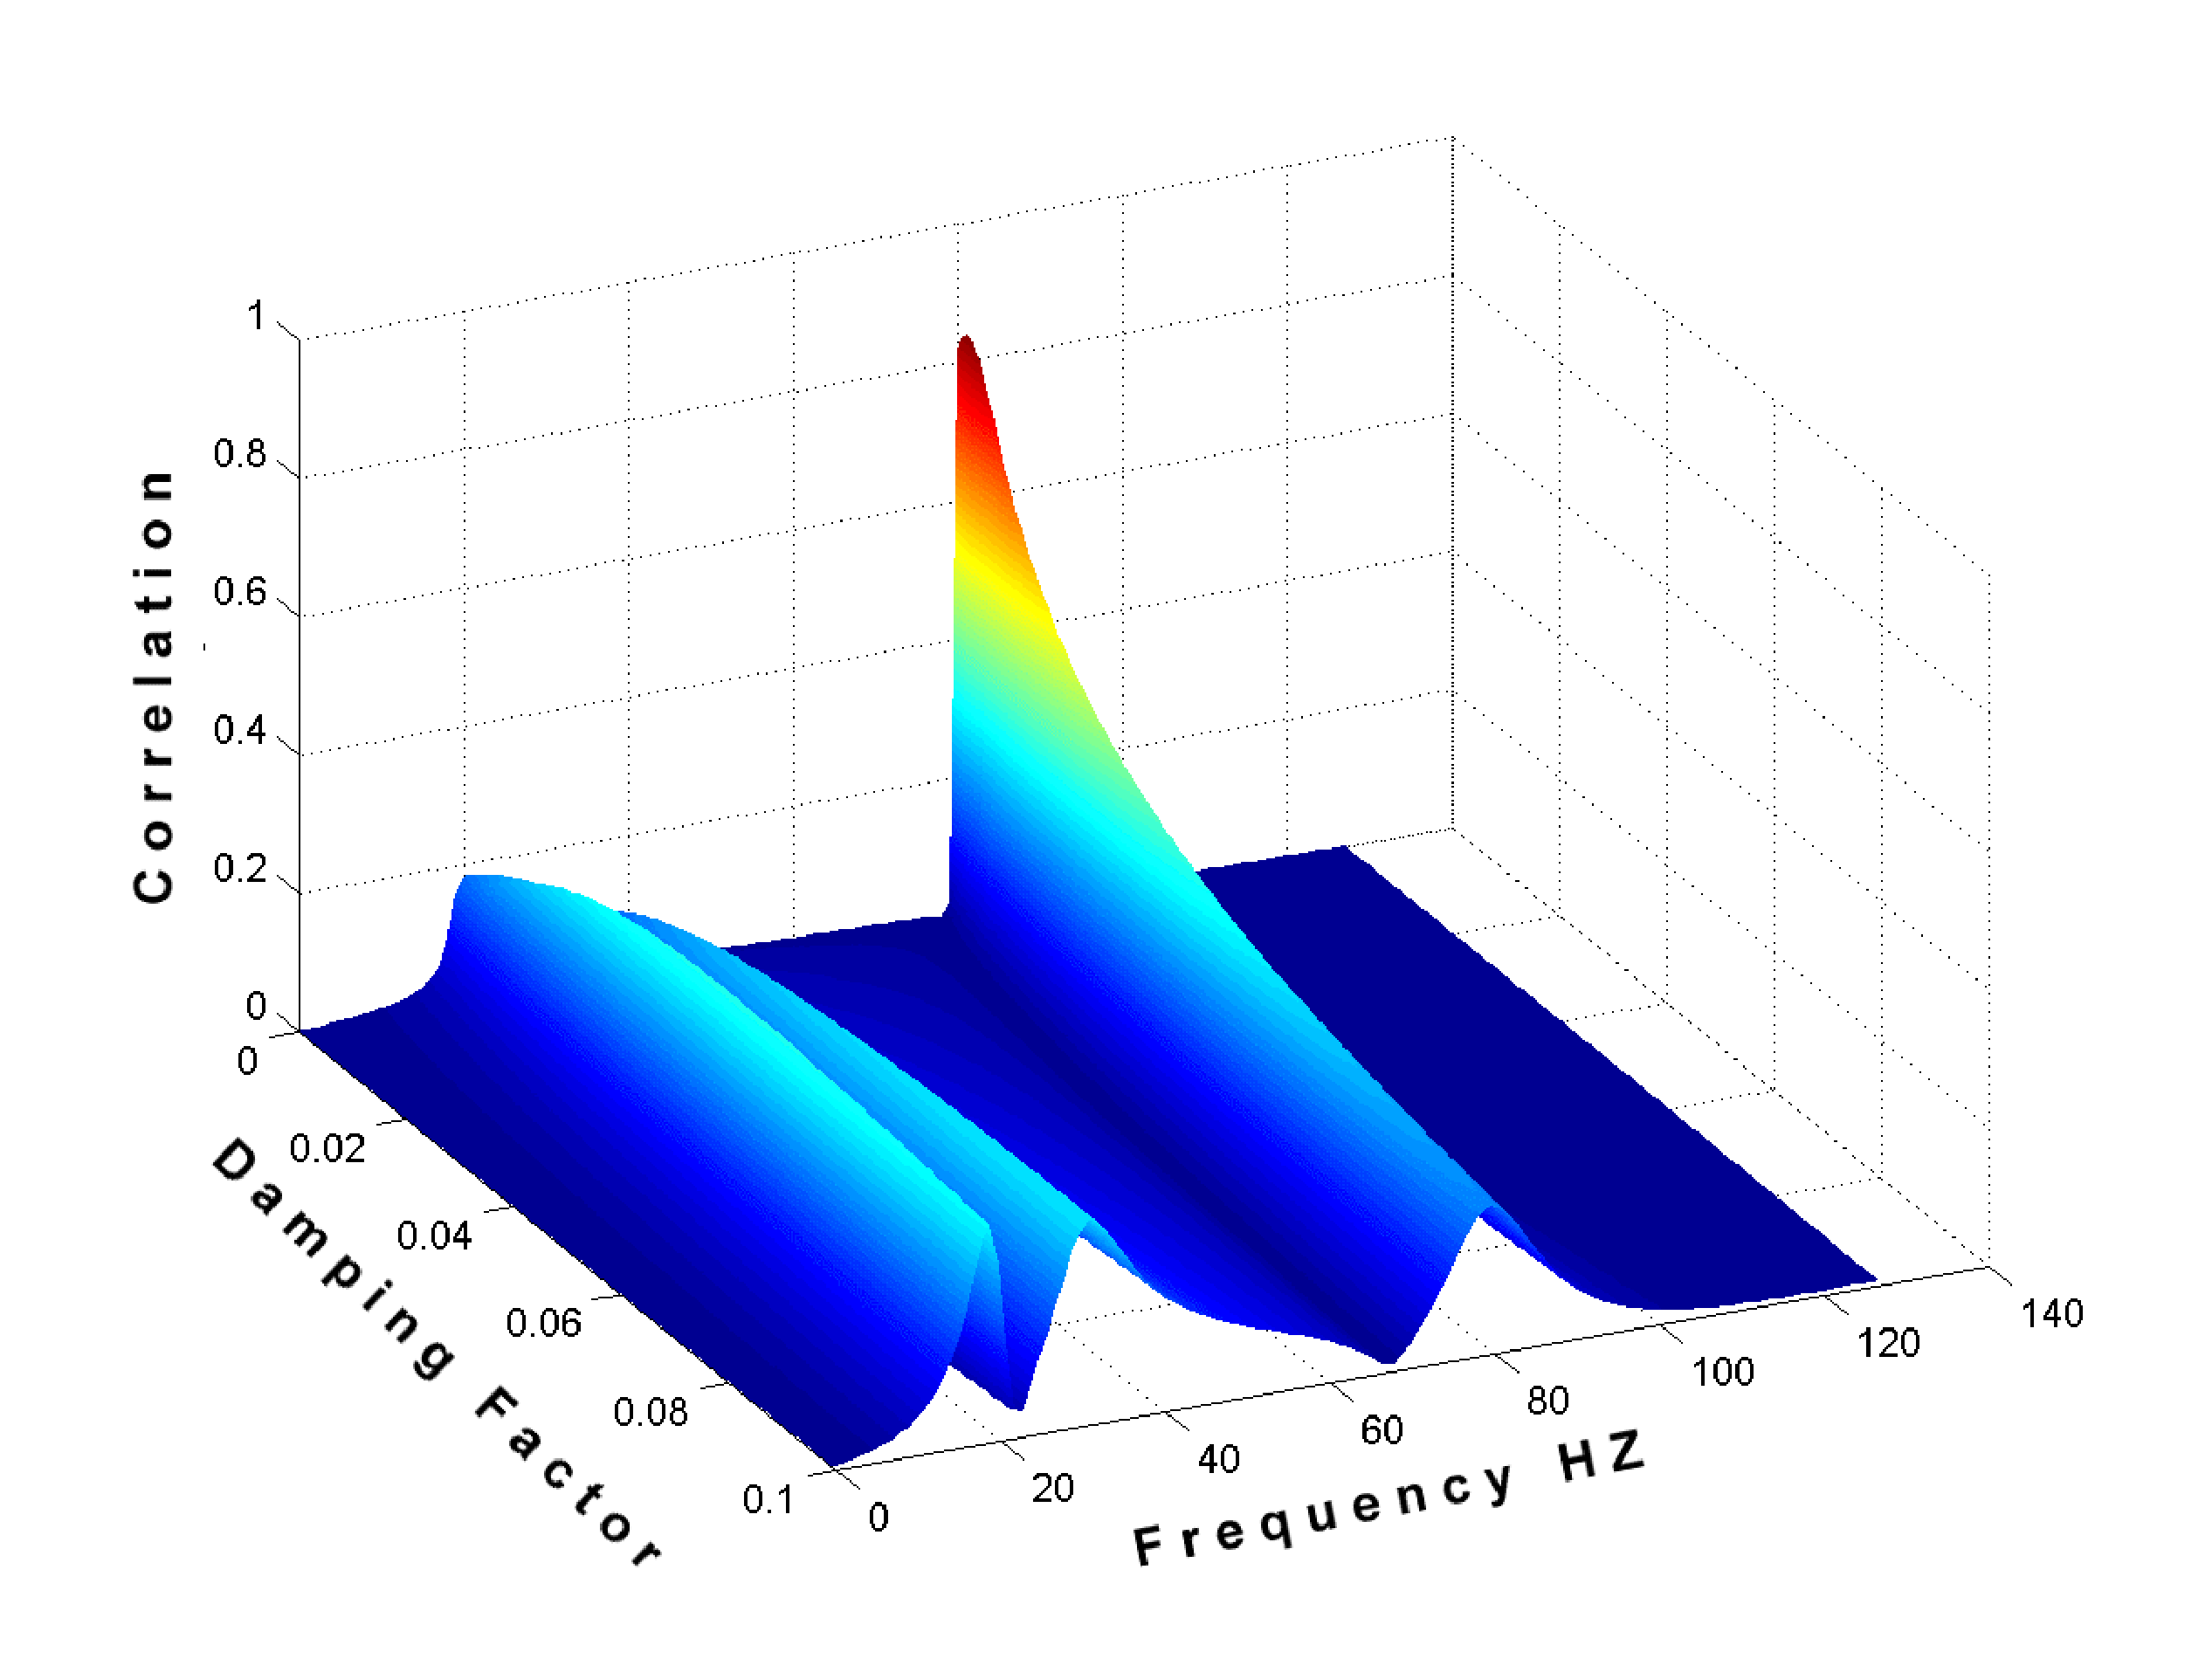
\includegraphics[keepaspectratio=true,scale=0.3]{figuras/fig01.eps}
	\caption{Wavelets correlation coefficients}
\end{figure}

\section{Tabela}

As tabelas devem estar centradas entre margens e identificadas por uma legenda 
alinhada a esquerda, com recuo especial de deslocamento de 1,8 cm, posicionada 
acima da tabela com mostrado nas Tabs. (\ref{tab01}) e (2), a título de 
exemplo. O tamanho das fontes empregadas nos rótulos e anotações usadas nas 
tabelas deve ser compatível com o usado no corpo do texto. Rótulos e anotações 
devem estar em português. Um espaçamento de 11 pts deve ser deixado entre a 
legenda e a tabela, bem como após a tabela. 

As grandezas dimensionais mostradas em cada tabela devem apresentar unidades 
consistentes com o SI. As unidades de cada variável devem ser mostradas apenas 
na primeira linha e/ou coluna da tabela, entre colchetes 

A referência explícita no texto à uma dada tabela deve ser feita como 
\lq\lq Tab. (\ref{tab01})\rq\rq\ quando no meio de uma frase ou como 
\lq\lq Tabela (\ref{tab01})\rq\rq\ quando no início da mesma. Referências 
implícitas a uma dada tabela devem ser feitas entre parênteses como 
\lq\lq (Tab. \ref{tab01}). Para referências a mais de uma tabela as mesmas 
regras devem ser aplicadas usando-se o plural adequadamente. Exemplos:
\begin{itemize}
	\item \lq\lq Após os ensaios experimentais, foram obtidos os resultados 
	mostrados na Tab. (\ref{tab01}), que ...\rq\rq
	\item \lq\lq A Tabela (\ref{tab01}) apresenta os resultados obtidos, onde 
	pode-se observar que ...\rq\rq
	\item As Tabelas (1) a (3) apresentam os resultados obtidos, ...\rq\rq
	\item Verificou-se uma forte dependência entre as variáveis citadas 
	(Tab. \ref{tab01}), comprovando ...\rq\rq
\end{itemize}

Cada tabela deve ser posicionada o mais próxima possível da primeira citação 
feita à mesma no texto, imediatamente após o parágrafo no qual é feita a 
citação, se possível, na mesma página.

\begin{table}[h]
	\centering
	\label{tab01}
	
	\begin{tabular}{ccc}
		\toprule
		\textbf{Processing type} & \textbf{Property 1} (\%) & 
		\textbf{Property 2} $[\mu m]$ \\
		\midrule
		Process 1 & 40.0 & 22.7 \\
		Process 2 & 48.4 & 13.9 \\
		Process 3 & 39.0 & 22.5 \\
		Process 4 & 45.3 & 28.5 \\
		\bottomrule
	\end{tabular}

	\caption{Propriedades obtidades após processamento}
\end{table}

\section{Citação de Referências}

Referencias a outros trabalhos tais como artigos, teses, relatórios, etc. devem 
ser feitas no corpo do texto devem estar de acordo com a norma corrente ABNT 
NBR 6023:2002 (ABNT, 2000), esta ultima baseada nas normas ISO 690:1987:
\begin{itemize}
	\item \lq\lq \cite{bordalo1989}, mostraram que...\rq\rq

	\item \lq\lq Resultados disponíveis em \cite{coimbra1978}, \cite{clark1986} 
	e \cite{sparrow1980}, mostram que...\rq\rq
\end{itemize}

Para referências a trabalhos com até dois autores, deve-se citar o nome de 
ambos os autores, por exemplo: \lq\lq \cite{soviero1997}, mostraram 
que...\rq\rq


%\chapter[Elementos do Pós-Texto]{Elementos do Pós-Texto}

Este capitulo apresenta instruções gerais sobre a elaboração e formatação dos 
elementos do pós-texto a serem apresentados em relatórios de Projeto de 
Graduação. São abordados aspectos relacionados a redação de referências 
bibliográficas, bibliografia, anexos e contra-capa.

\section{Referências Bibliográficas}

O primeiro elemento do pós-texto, inserido numa nova página, logo após o último 
capítulo do trabalho, consiste da lista das referencias bibliográficas citadas 
ao longo do texto.

Cada referência na lista deve ser justificada entre margens e redigida no 
formato Times New Roman com 11pts. Não é necessário introduzir uma linha em 
branco entre referências sucessivas.

A primeira linha de cada referencia deve ser alinhada a esquerda, com as demais 
linhas da referencia deslocadas de 0,5 cm a partir da margem esquerda. 

Todas as referências aparecendo na lista da seção \lq\lq Referências 
Bibliográficas\rq\rq\ devem estar citadas no texto. Da mesma forma o autor deve 
verificar que não há no corpo do texto citação a referências que por 
esquecimento não forma incluídas nesta seção.

As referências devem ser listadas em ordem alfabética, de acordo com o último 
nome do primeiro autor. Alguns exemplos de listagem de referencias são 
apresentados no Anexo I.

Artigos que ainda não tenham sido publicados, mesmo que tenham sido submetidos 
para publicação, não deverão ser citados. Artigos ainda não publicados mas que 
já tenham sido aceitos para publicação devem ser citados como \lq\lq in 
press\rq\rq.

A norma \cite{NBR6034:2000}, que regulamenta toda a formatação a ser usada na 
elaboração de referências a diferente tipos de fontes de consulta, deve ser 
rigidamente observada. Sugere-se a consulta do trabalho realizado por 
\cite{arruda2007}, disponível na internet.

\section{Anexos}

As informações citadas ao longo do texto como \lq\lq Anexos\rq\rq\ devem ser 
apresentadas numa seção isolada ao término do trabalho, após a seção de 
referências bibliográficas. Os anexos devem ser numerados seqüencialmente em 
algarismos romanos maiúsculos (I, II, III, ...). A primeira página dos anexos 
deve apresentar um índice conforme modelo apresentado no Anexo I, descrevendo 
cada anexo e a página inicial do mesmo.

A referência explícita no texto à um dado anexo deve ser feita como 
\lq\lq Anexo 1\rq\rq. Referências implícitas a um dado anexo devem ser feitas 
entre parênteses como (Anexo I). Para referências a mais de um anexo as mesmas 
regras devem ser aplicadas usando-se o plural adequadamente. Exemplos:
\begin{itemize}
	\item \lq\lq Os resultados detalhados dos ensaios experimentais são 
	apresentados no Anexo IV, onde ...\rq\rq

	\item \lq\lq O Anexo I apresenta os resultados obtidos, onde pode-se 
	observar que ...\rq\rq

	\item \lq\lq Os Anexos I a IV apresentam os resultados obtidos ...\rq\rq

	\item \lq\lq Verificou-se uma forte dependência entre as variáveis citadas 
	(Anexo V), comprovando ...\rq\rq
\end{itemize}




\bookmarksetup{startatroot} 

\postextual

\bibliography{bibliografia} 
\begin{apendicesenv}

\partapendices

\chapter{Exemplo de Uso 1} \label{apendice:eu1}
\section{$L(S)$} \label{apendice:eu1:LS}
\lstinputlisting{dados/eu1_LS}

\chapter{Exemplo de Uso 2} \label{apendice:eu2}
\section{$S$} \label{apendice:eu2:S}
\lstinputlisting{dados/eu2_S_da_avaliacao}
\section{$L(S)$} \label{apendice:eu2:LS}
\lstinputlisting{dados/eu2_LS}
\section{$L(f)$} \label{apendice:eu2:Lf}
\lstinputlisting{dados/eu2_Lf}
\section{Positivos} \label{apendice:eu2:positivo}
\lstinputlisting{dados/eu2_positivo}
\section{Falsos Positivos} \label{apendice:eu2:falso_positivo}
\lstinputlisting{dados/eu2_falso_positivo}
\section{Falsos Negativos} \label{apendice:eu2:falso_negativo}
\lstinputlisting{dados/eu2_falso_negativo}
%\lstinputlisting{dados/eu2_framac_raw_report}


\end{apendicesenv}

%\begin{anexosenv}

\partanexos

\chapter{Análise dos Percentis do Estudo de Caso} \label{anex:percentis}

Neste anexo contém os gráficos relacionados com a análise de percentis de cada
uma das métricas de vulnerabilidades apresentadas em \ref{cap:metricas_vuln}
do
projeto Linux, sendo esses parte dos resultados descritos na seção \ref{analise_estudo}.


\begin{figure}[h]
  \centering
  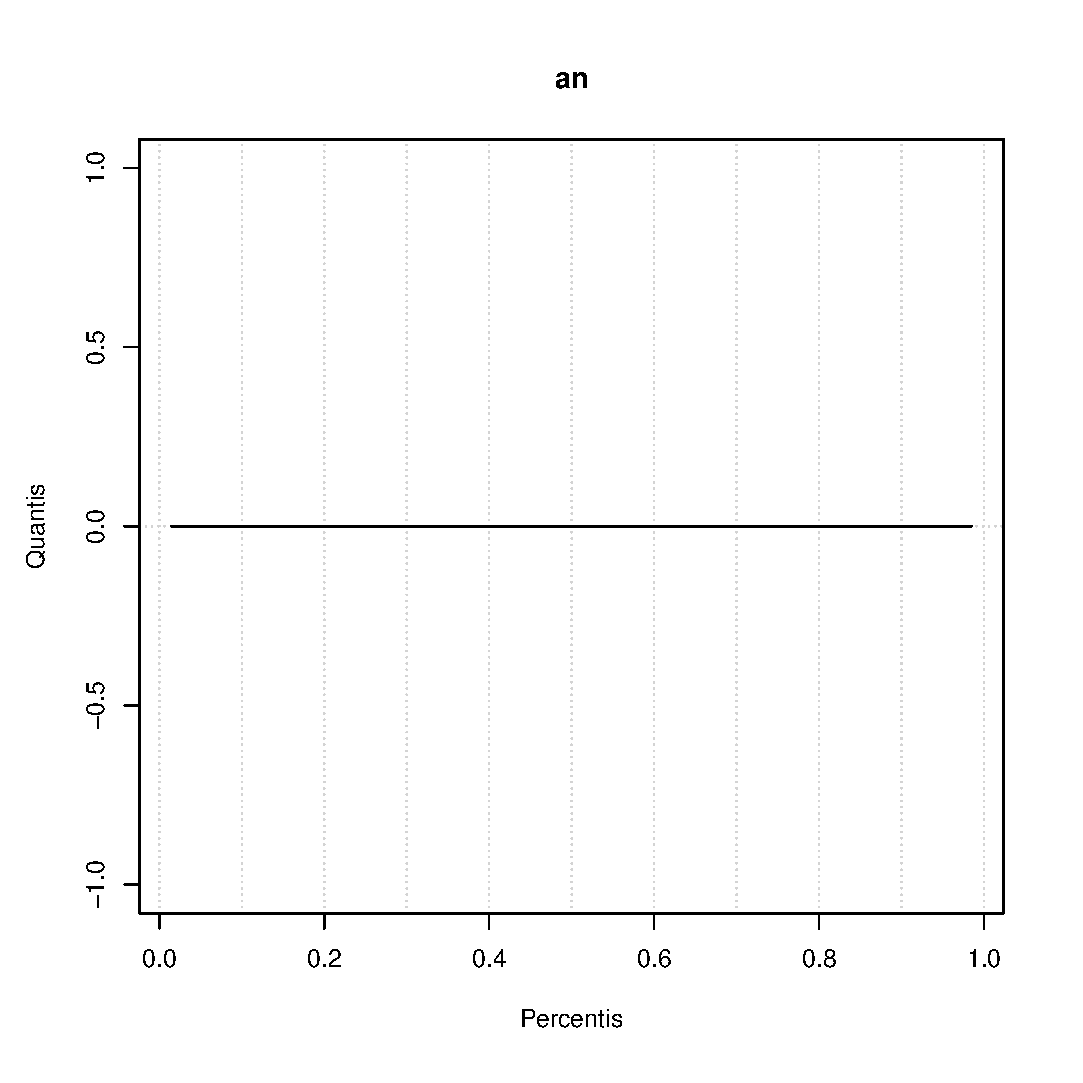
\includegraphics[width=0.7\textwidth]
      {dados/linux/an.eps}
  \caption{Gráfico de Percentis da métrica AN}
\end{figure}

\newpage

\begin{figure}[h]
  \centering
  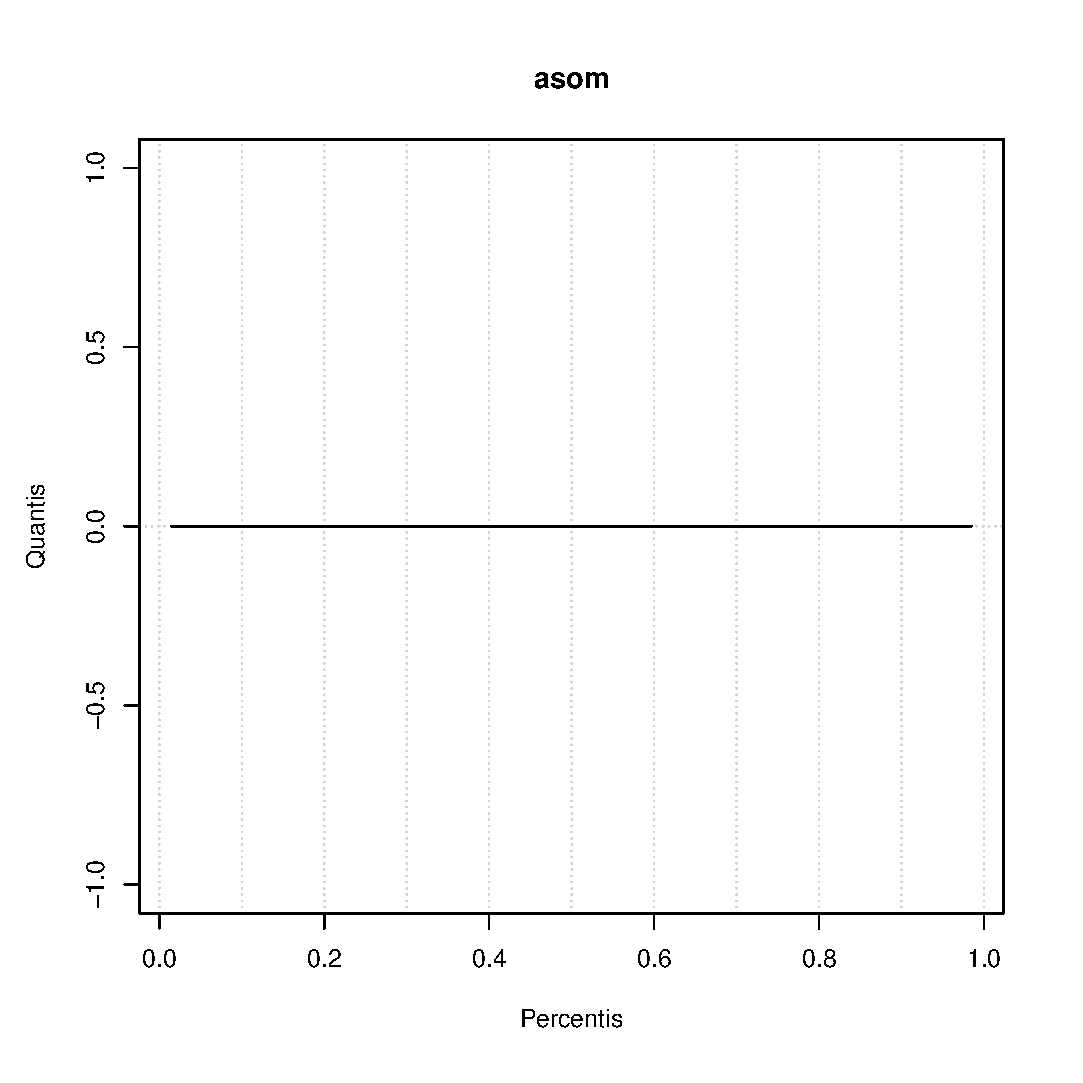
\includegraphics[width=0.6\textwidth]
      {dados/linux/asom.eps}
  \caption{Gráfico de Percentis da métrica ASOM}
  \label{graphic:asom}
\end{figure}

\begin{figure}[h]
  \centering
  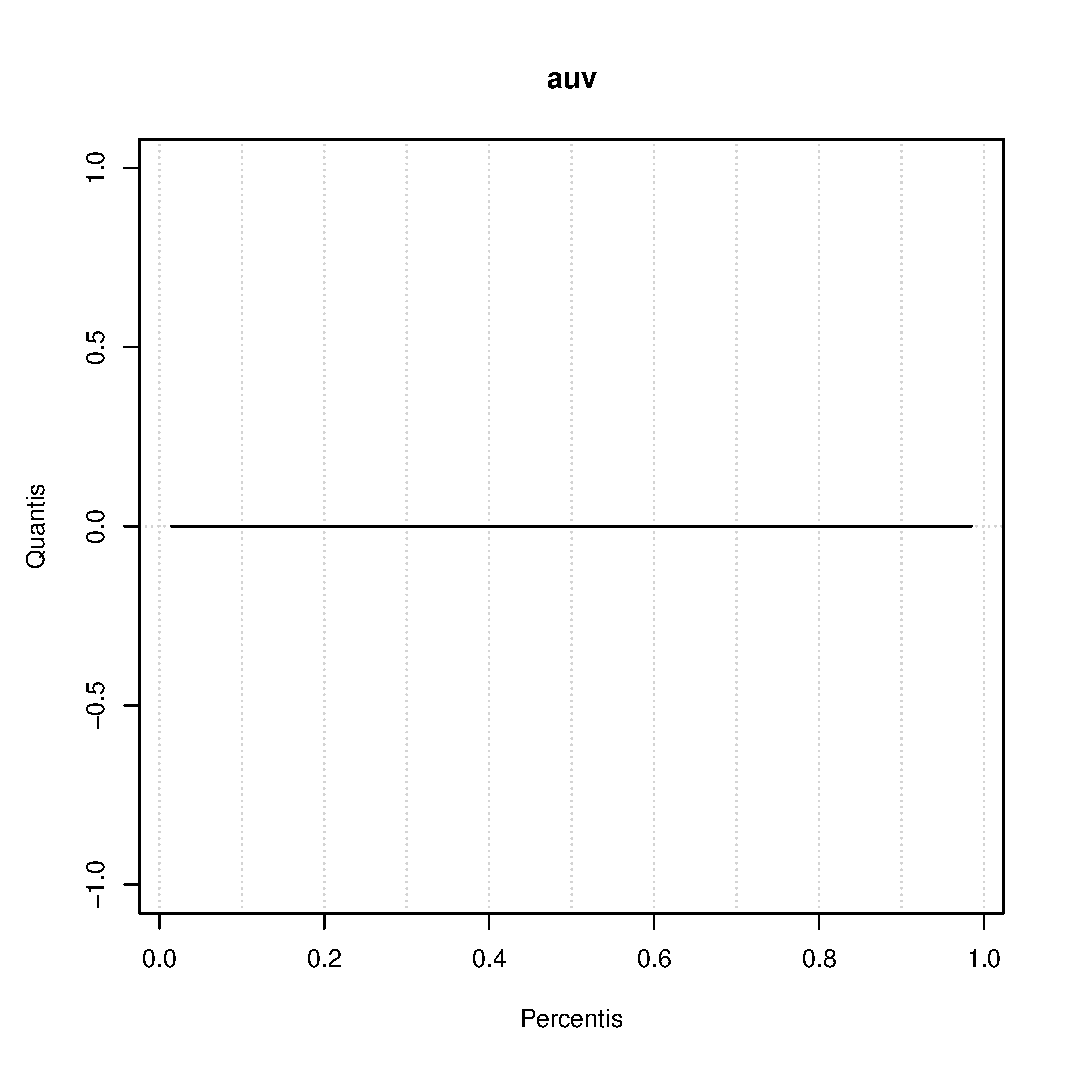
\includegraphics[width=0.6\textwidth]
      {dados/linux/auv.eps}
  \caption{Gráfico de Percentis da métrica AUV}
\end{figure}

\newpage

\begin{figure}[h]
  \centering
  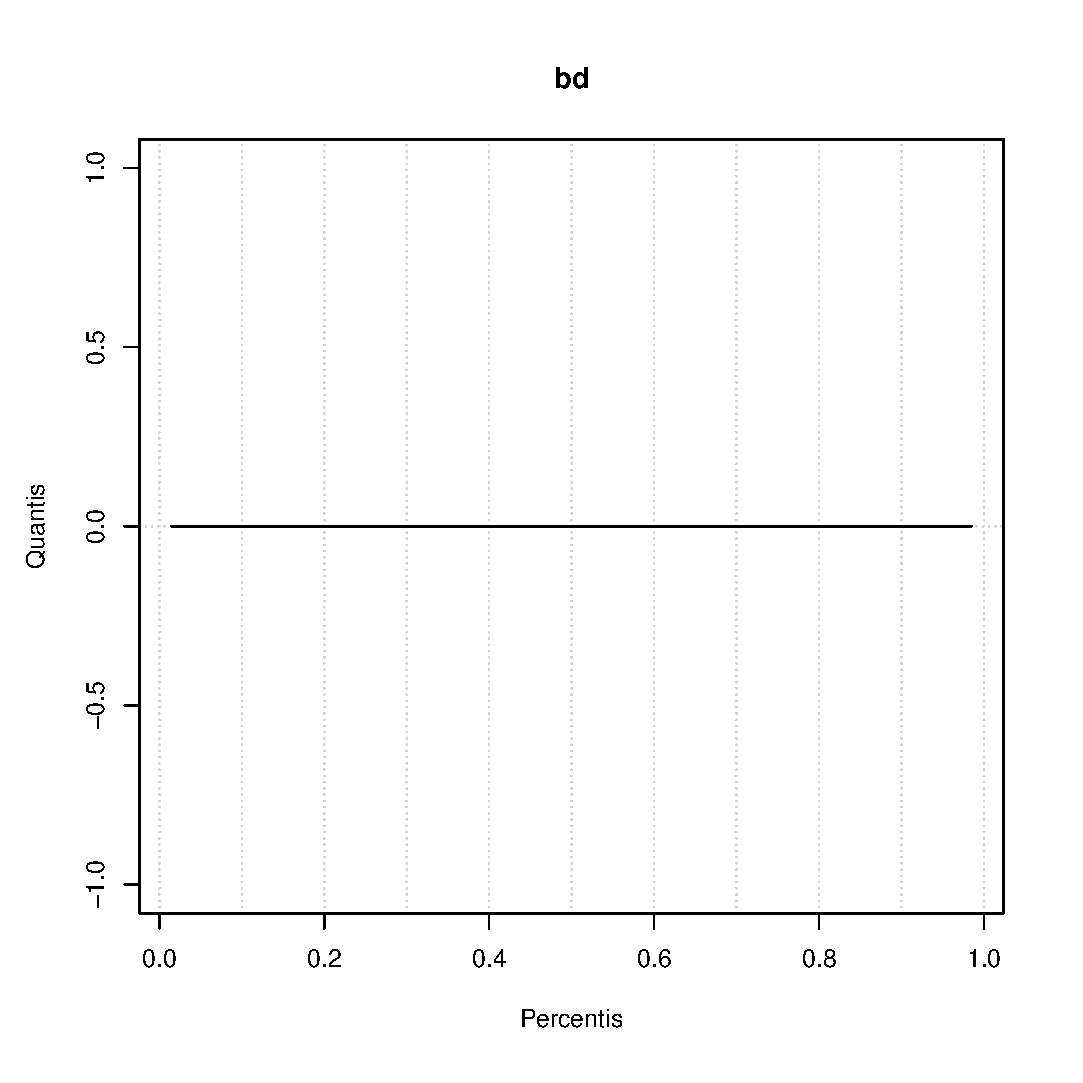
\includegraphics[width=0.6\textwidth]
      {dados/linux/bd.eps}
  \caption{Gráfico de Percentis da métrica BD}
\end{figure}

\begin{figure}[h]
  \centering
  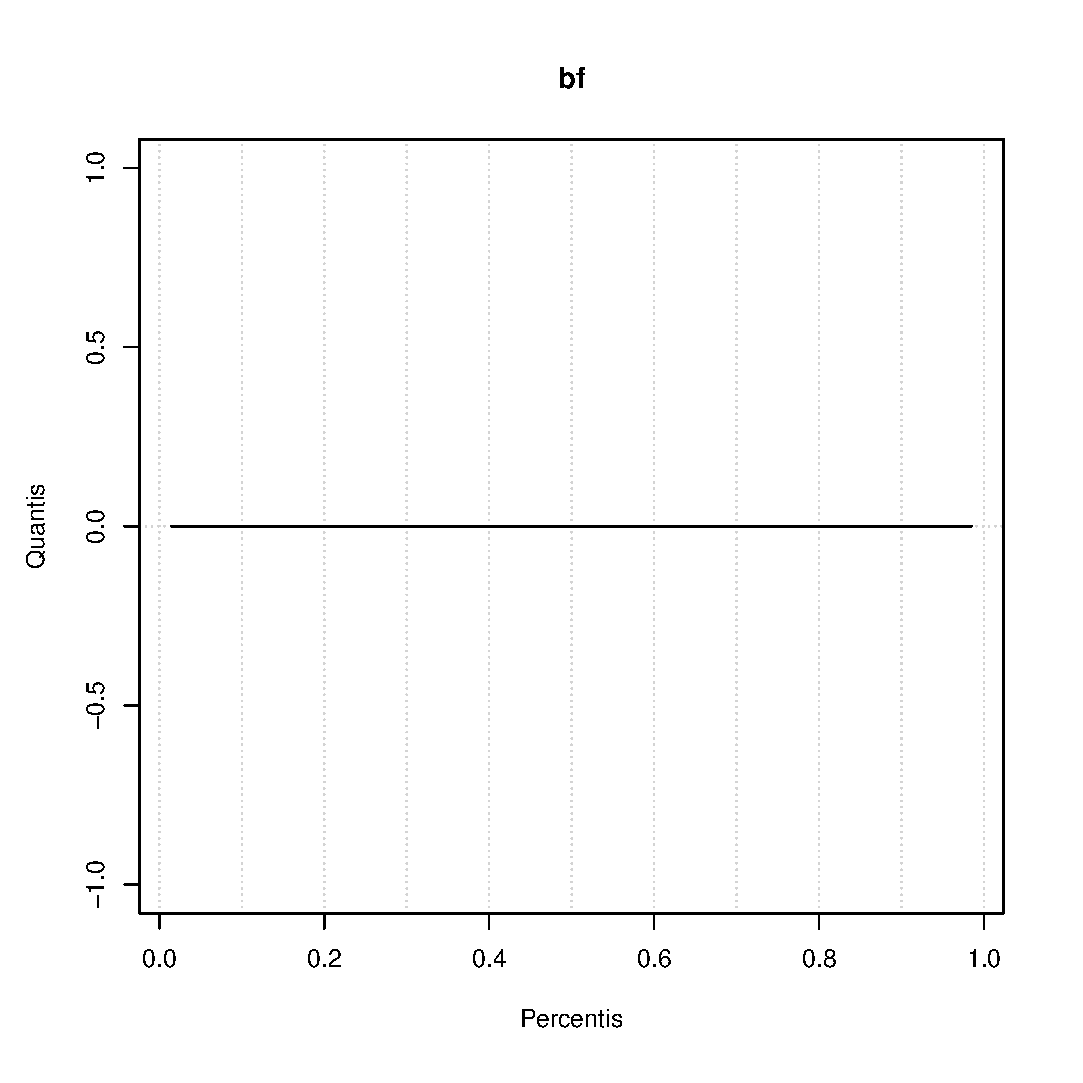
\includegraphics[width=0.6\textwidth]
      {dados/linux/bf.eps}
  \caption{Gráfico de Percentis da métrica BF}
\end{figure}

\newpage

\begin{figure}[h]
  \centering
  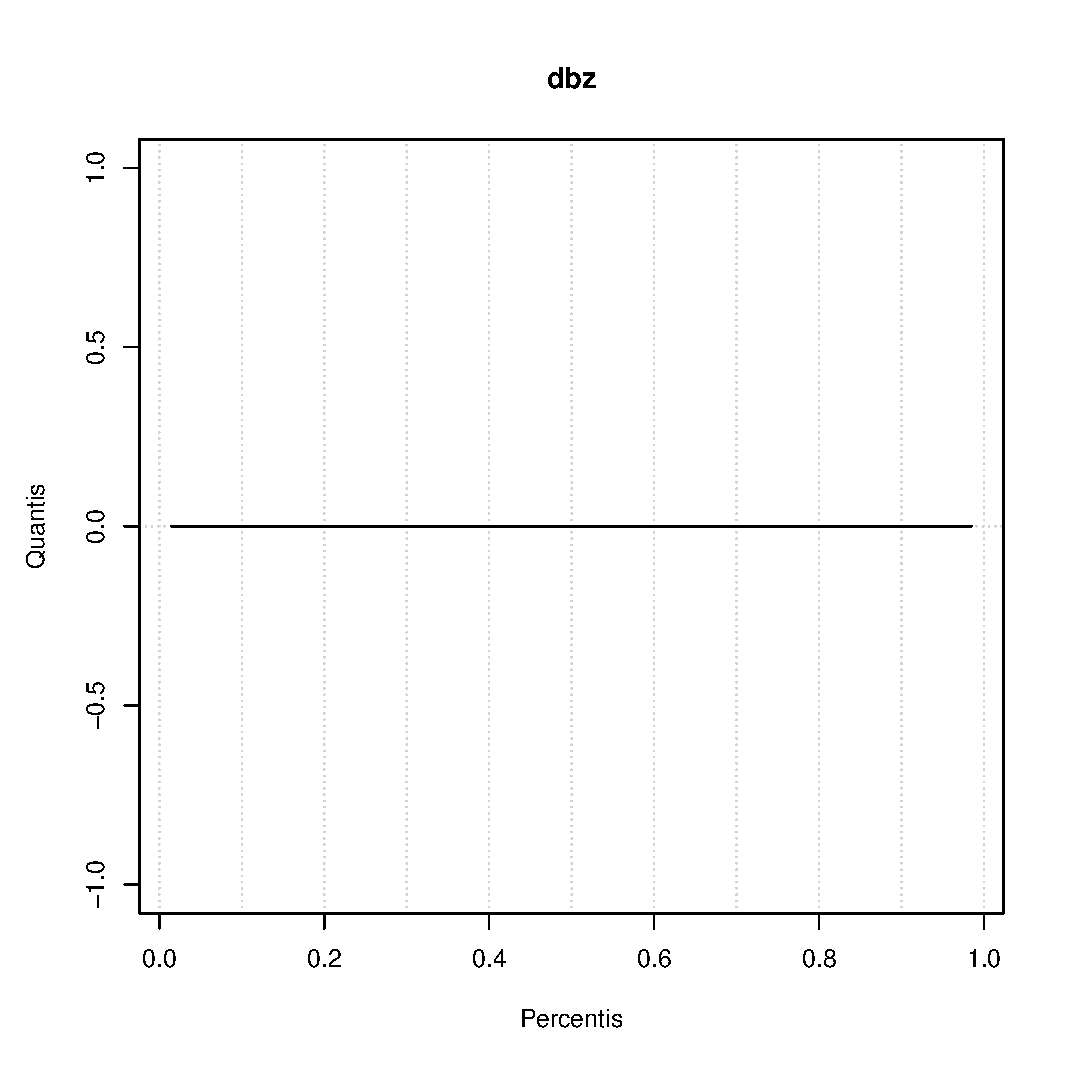
\includegraphics[width=0.6\textwidth]
      {dados/linux/dbz.eps}
  \caption{Gráfico de Percentis da métrica DBZ}
\end{figure}

\begin{figure}[h]
  \centering
  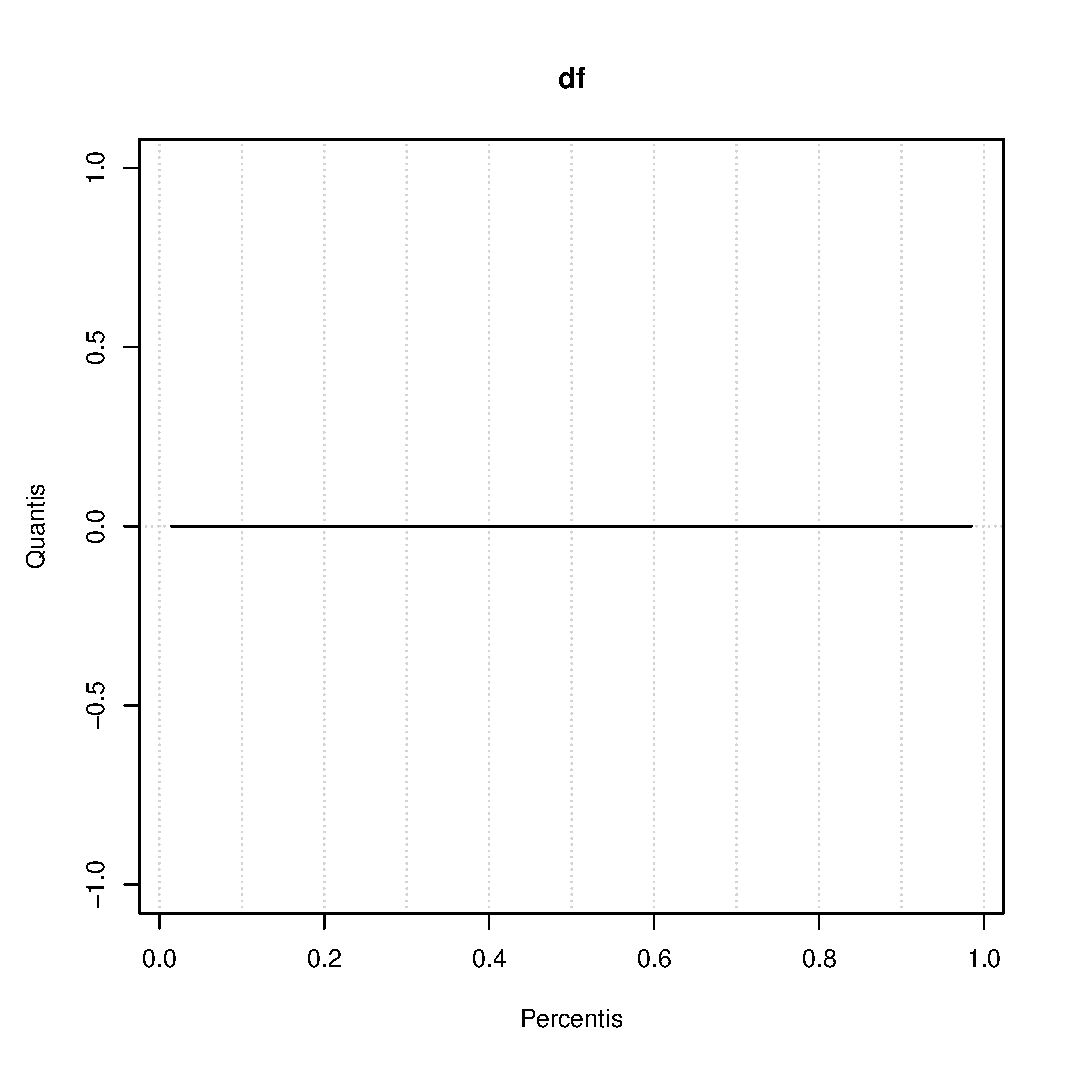
\includegraphics[width=0.6\textwidth]
      {dados/linux/df.eps}
  \caption{Gráfico de Percentis da métrica DF}
\end{figure}

\newpage

\begin{figure}[h]
  \centering
  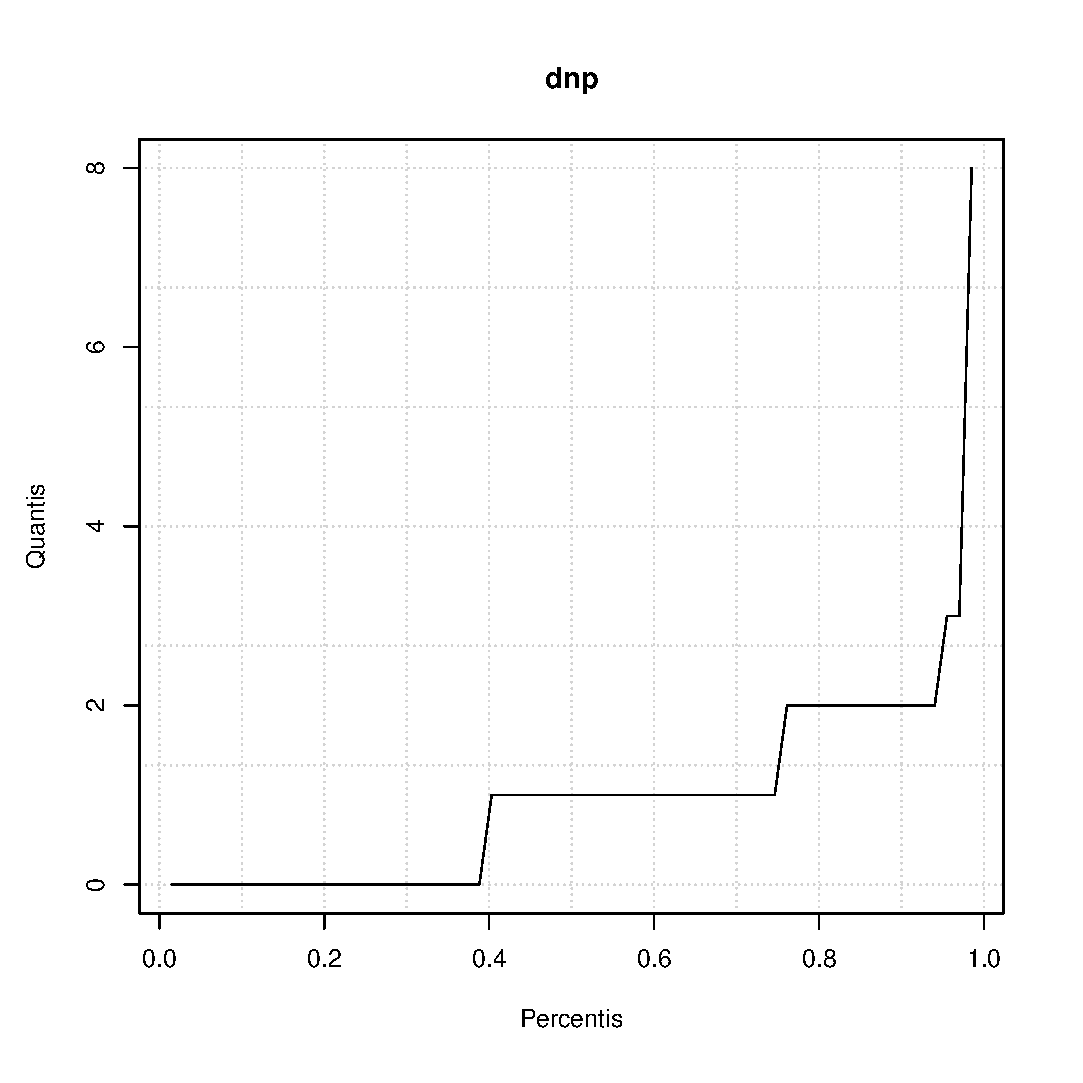
\includegraphics[width=0.6\textwidth]
      {dados/linux/dnp.eps}
  \caption{Gráfico de Percentis da métrica DNP}
  \label{graphic:dnp}
\end{figure}

\begin{figure}[h]
  \centering
  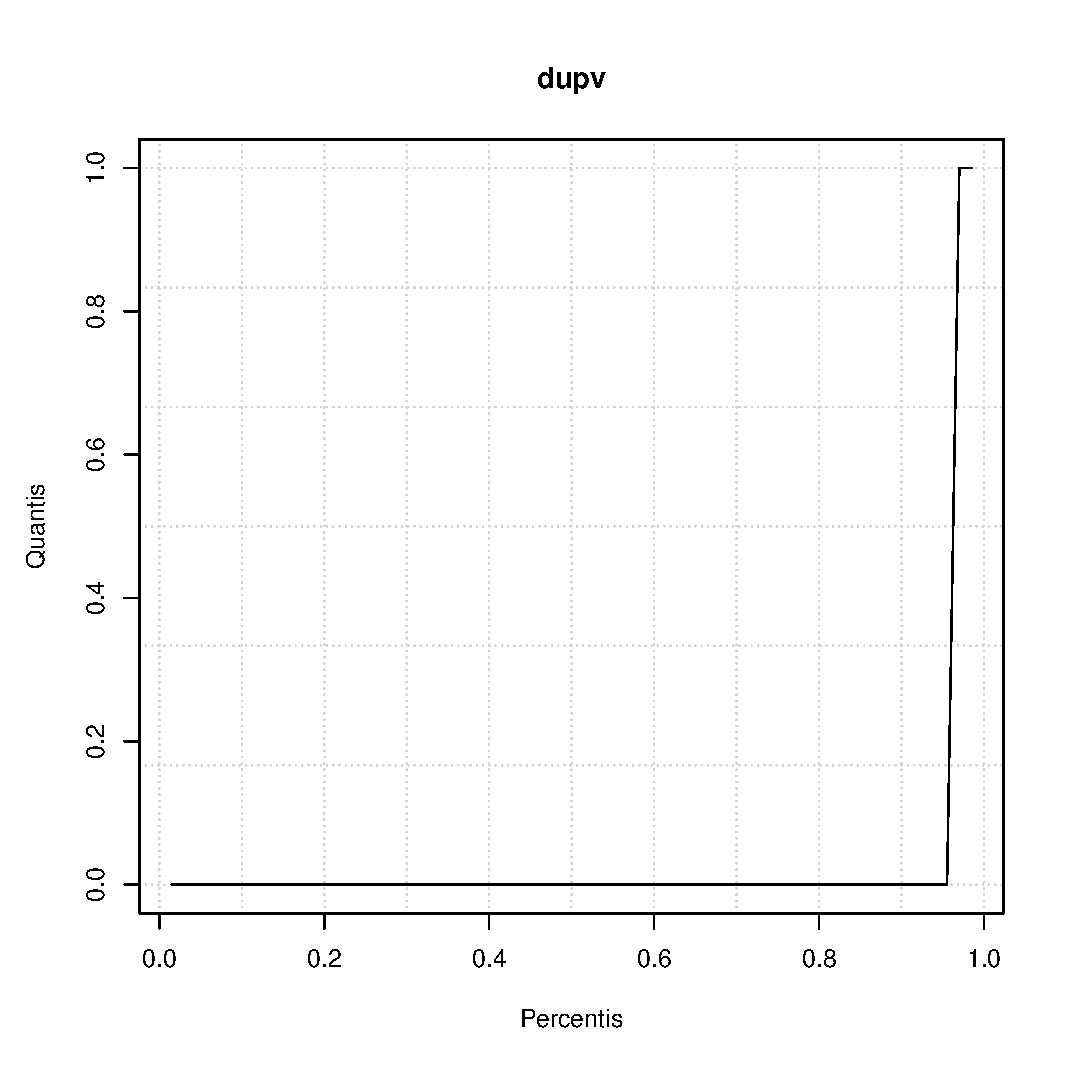
\includegraphics[width=0.6\textwidth]
      {dados/linux/dupv.eps}
  \caption{Gráfico de Percentis da métrica DUPV}
  \label{graphic:dupv}
\end{figure}

\newpage

\begin{figure}[h]
  \centering
  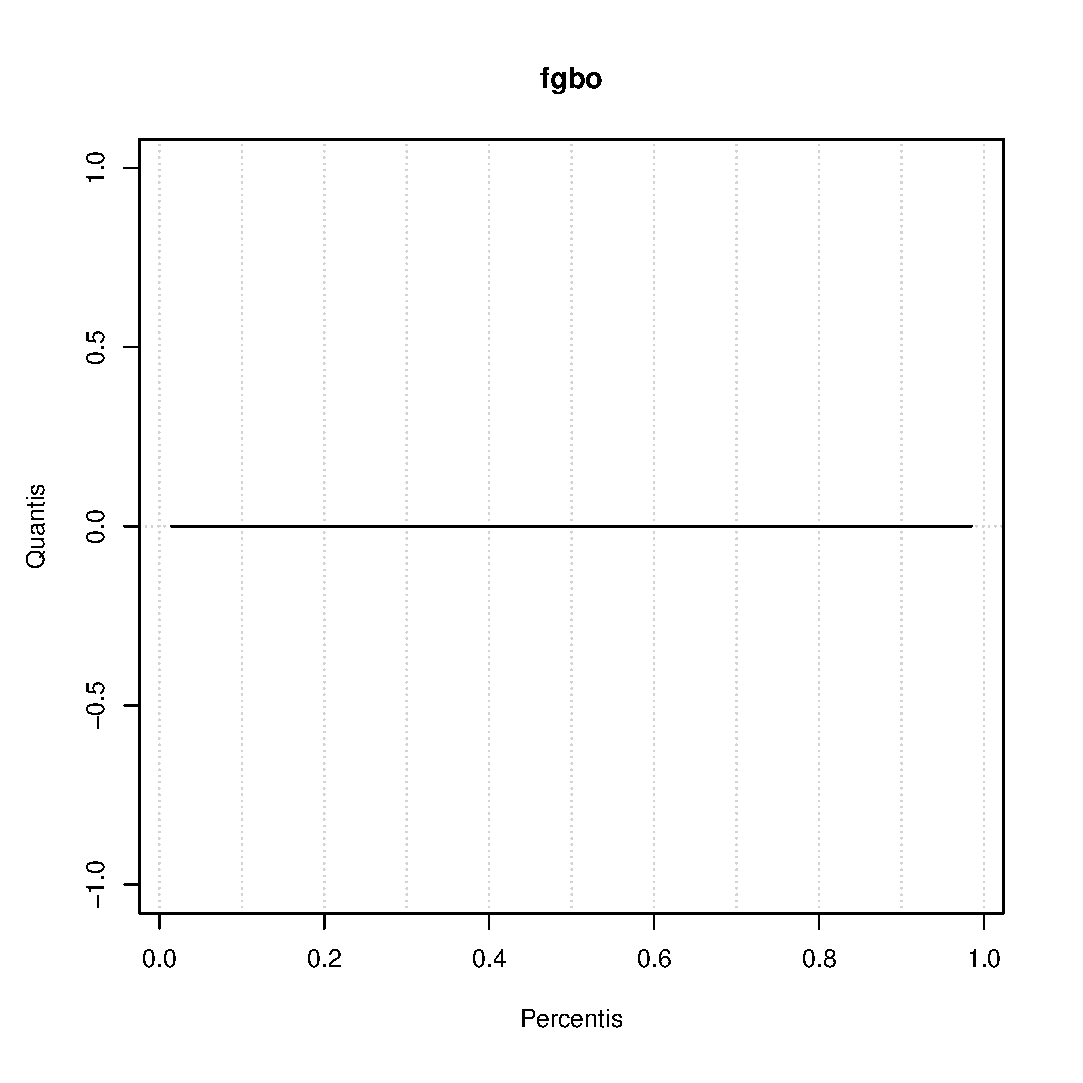
\includegraphics[width=0.6\textwidth]
      {dados/linux/fgbo.eps}
  \caption{Gráfico de Percentis da métrica FGBO}
\end{figure}

\begin{figure}[h]
  \centering
  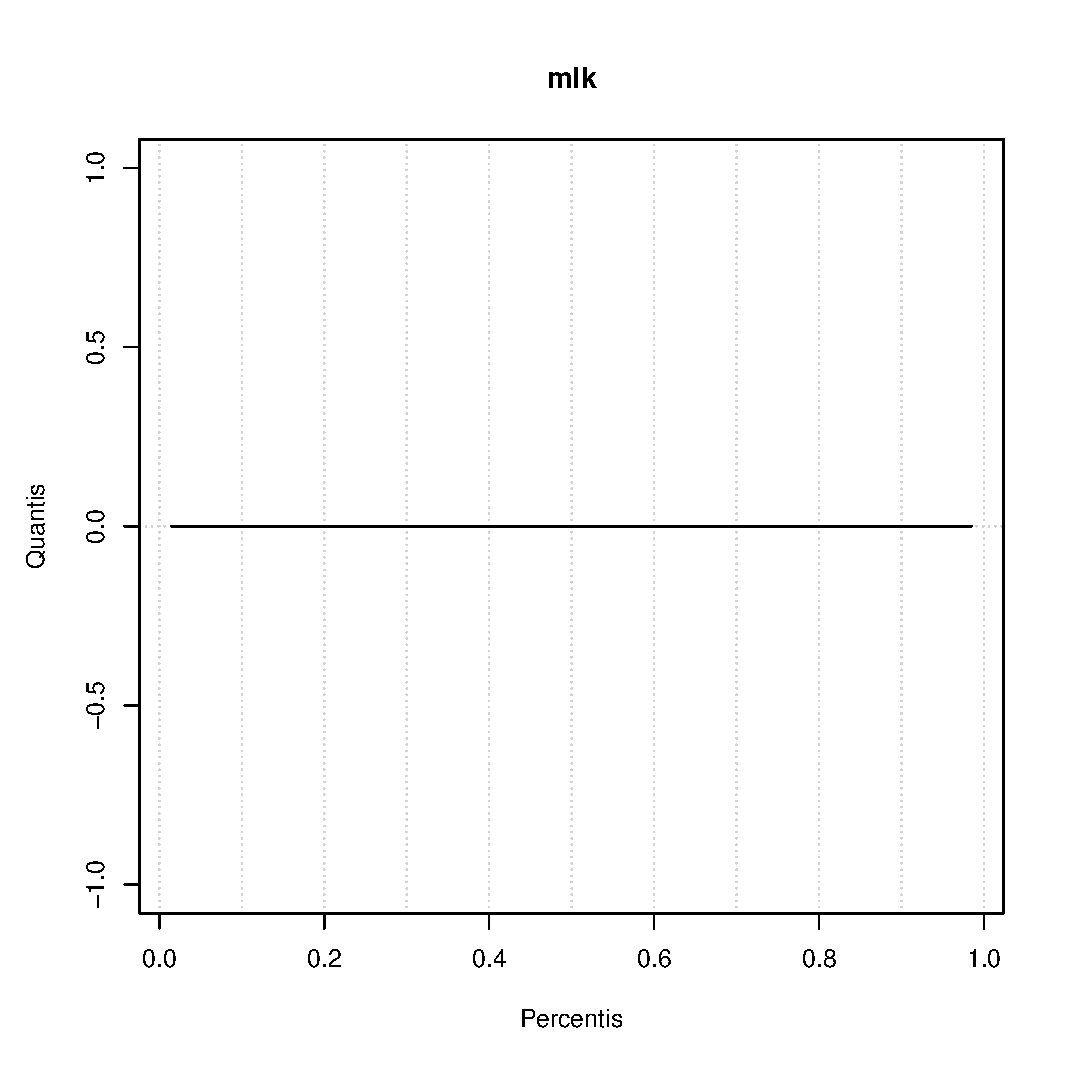
\includegraphics[width=0.6\textwidth]
      {dados/linux/mlk.eps}
  \caption{Gráfico de Percentis da métrica MLK}
\end{figure}

\newpage

\begin{figure}[h]
  \centering
  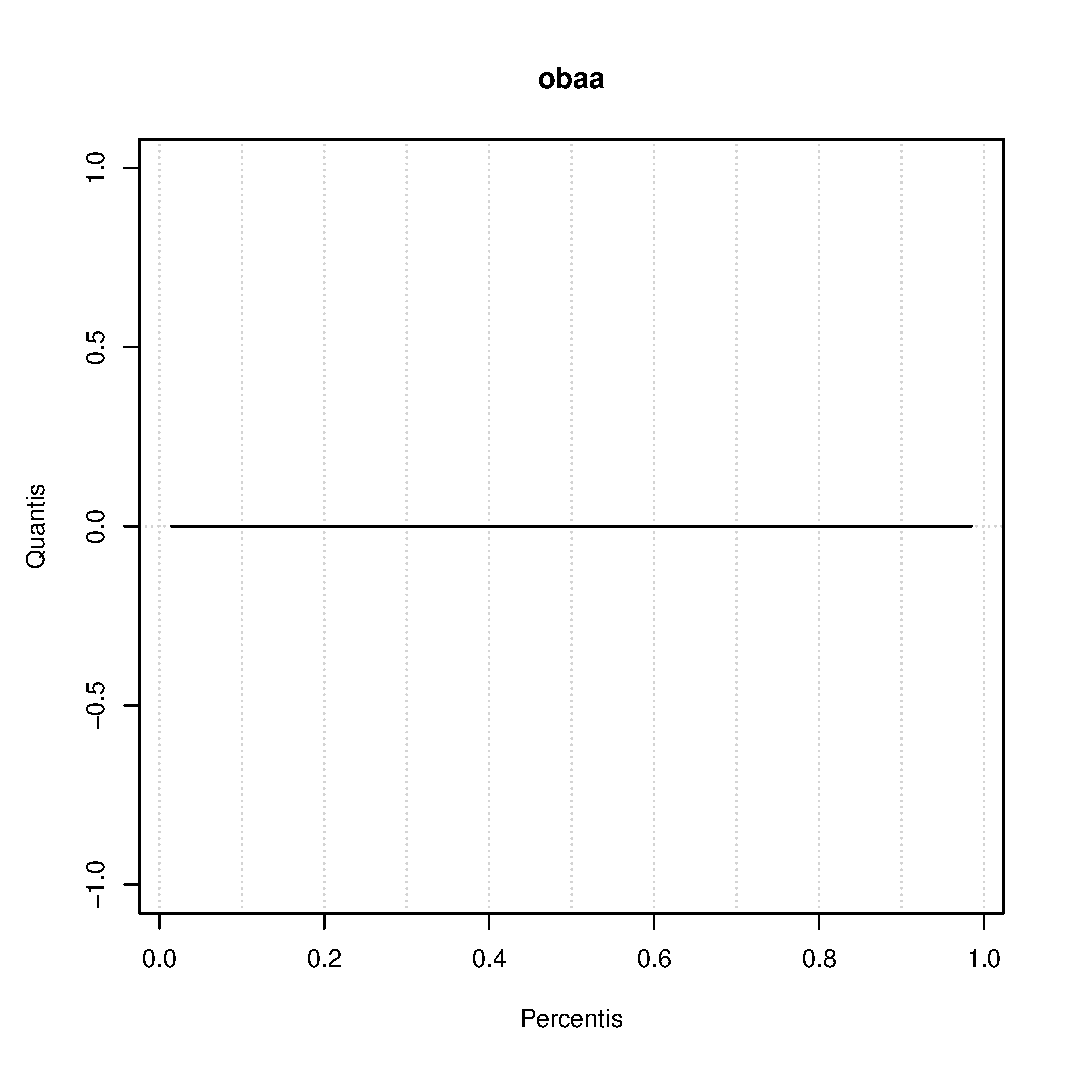
\includegraphics[width=0.6\textwidth]
      {dados/linux/obaa.eps}
  \caption{Gráfico de Percentis da métrica OBAA}
\end{figure}

\begin{figure}[h]
  \centering
  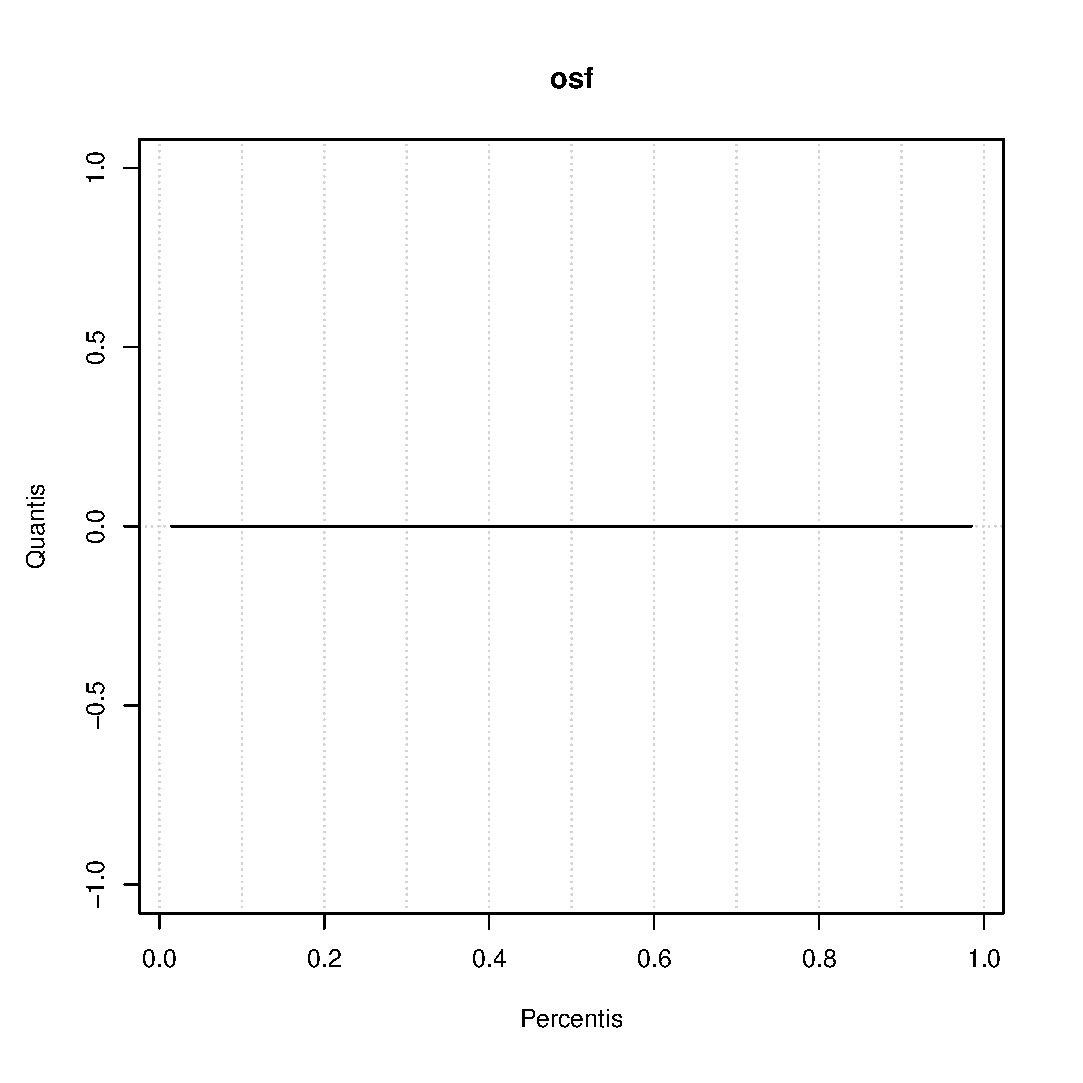
\includegraphics[width=0.6\textwidth]
      {dados/linux/osf.eps}
  \caption{Gráfico de Percentis da métrica OSF}
\end{figure}

\newpage

\begin{figure}[h]
  \centering
  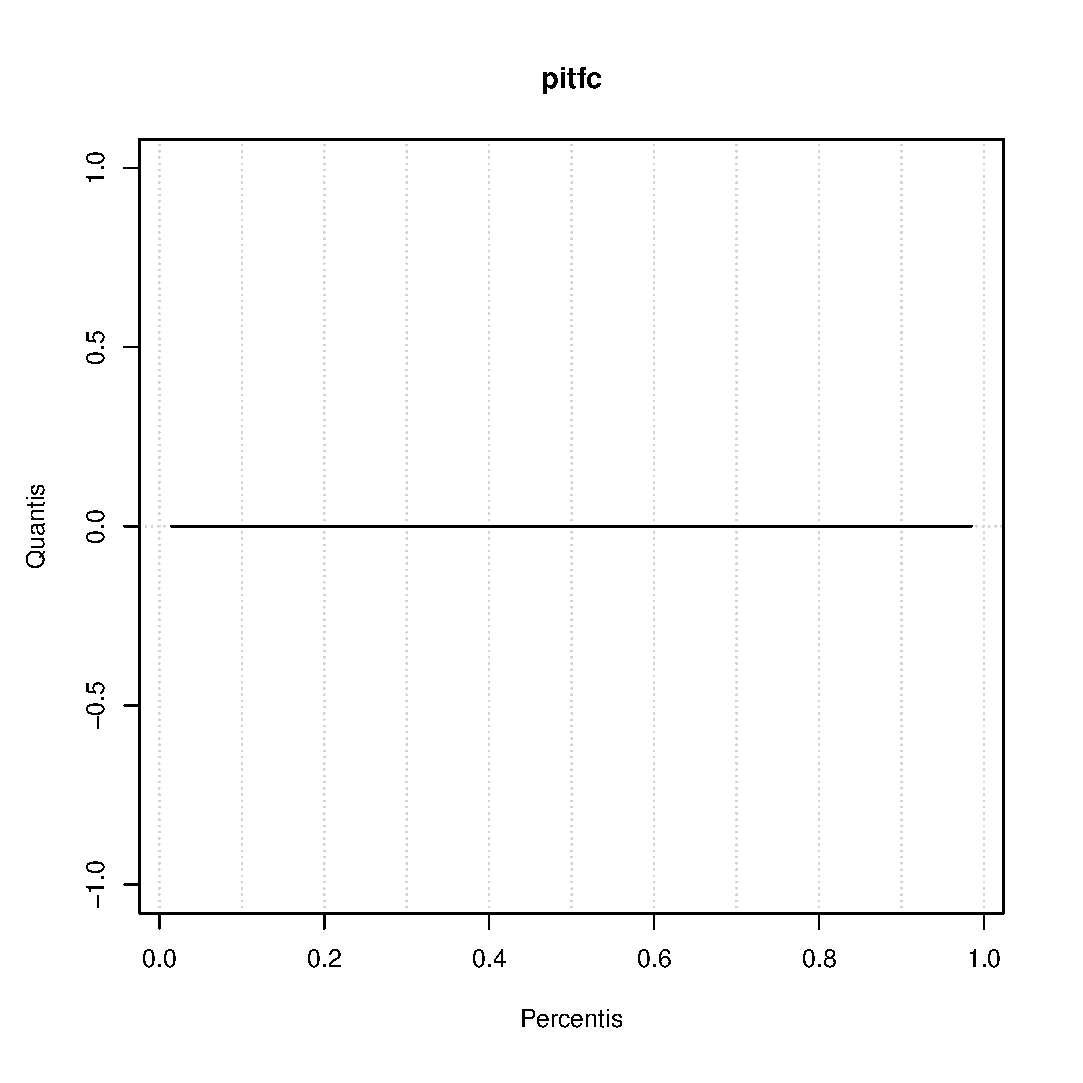
\includegraphics[width=0.6\textwidth]
      {dados/linux/pitfc.eps}
  \caption{Gráfico de Percentis da métrica PITFC}
\end{figure}

\begin{figure}[h]
  \centering
  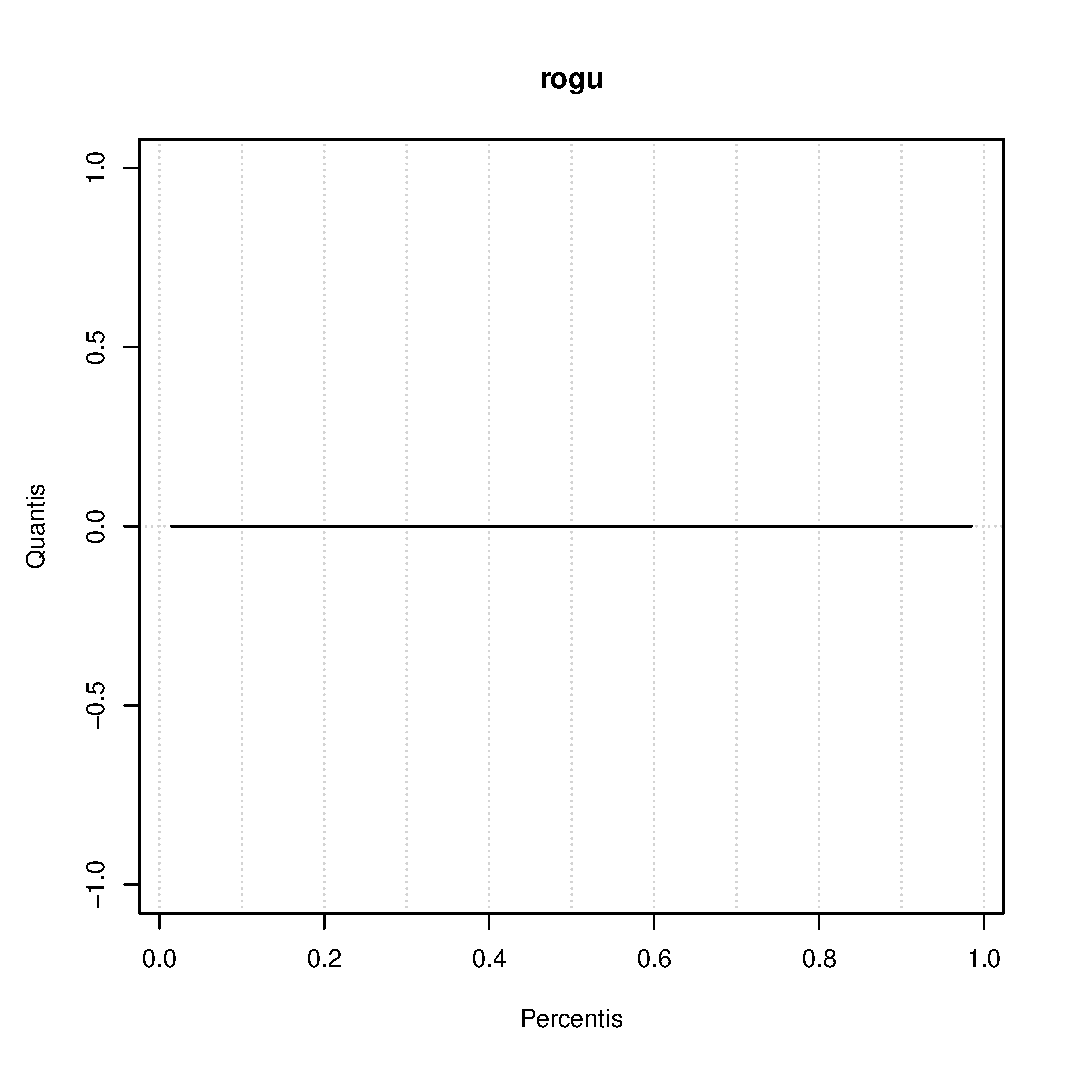
\includegraphics[width=0.6\textwidth]
      {dados/linux/rogu.eps}
  \caption{Gráfico de Percentis da métrica ROGU}
\end{figure}

\newpage

\begin{figure}[h]
  \centering
  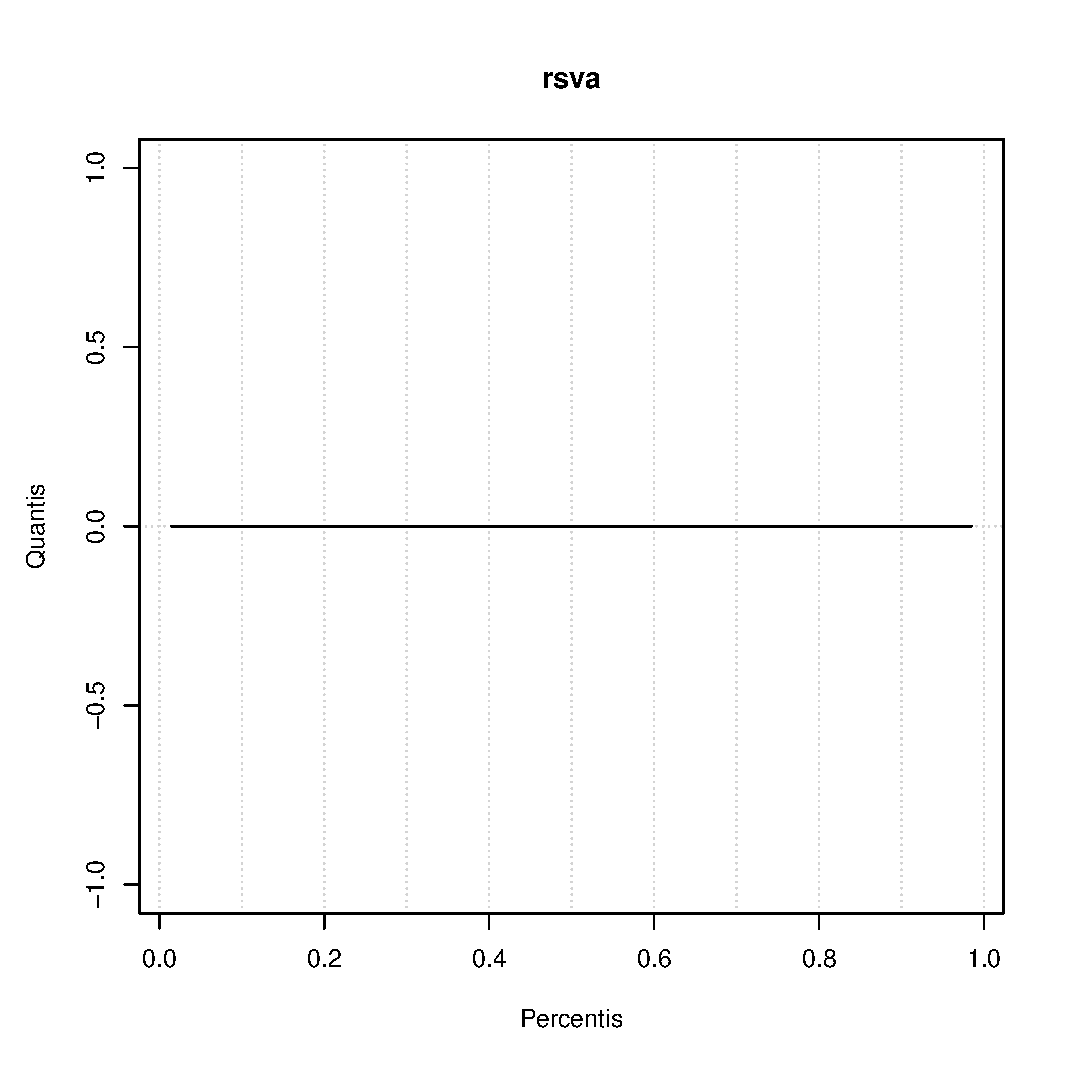
\includegraphics[width=0.6\textwidth]
      {dados/linux/rsva.eps}
  \caption{Gráfico de Percentis da métrica RSVA}
\end{figure}

\begin{figure}[h]
  \centering
  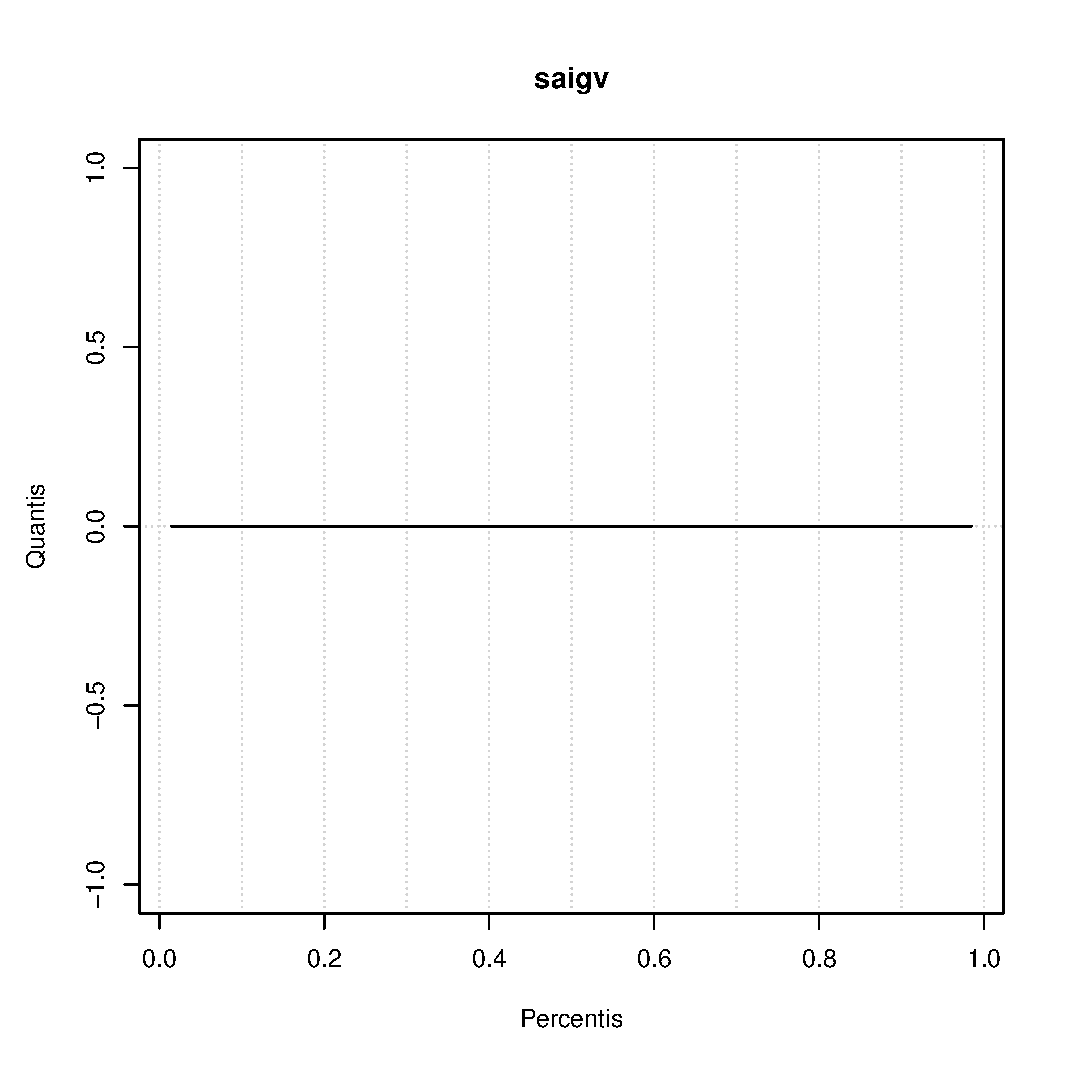
\includegraphics[width=0.6\textwidth]
      {dados/linux/saigv.eps}
  \caption{Gráfico de Percentis da métrica SAIGV}
\end{figure}

\newpage

\begin{figure}[h]
  \centering
  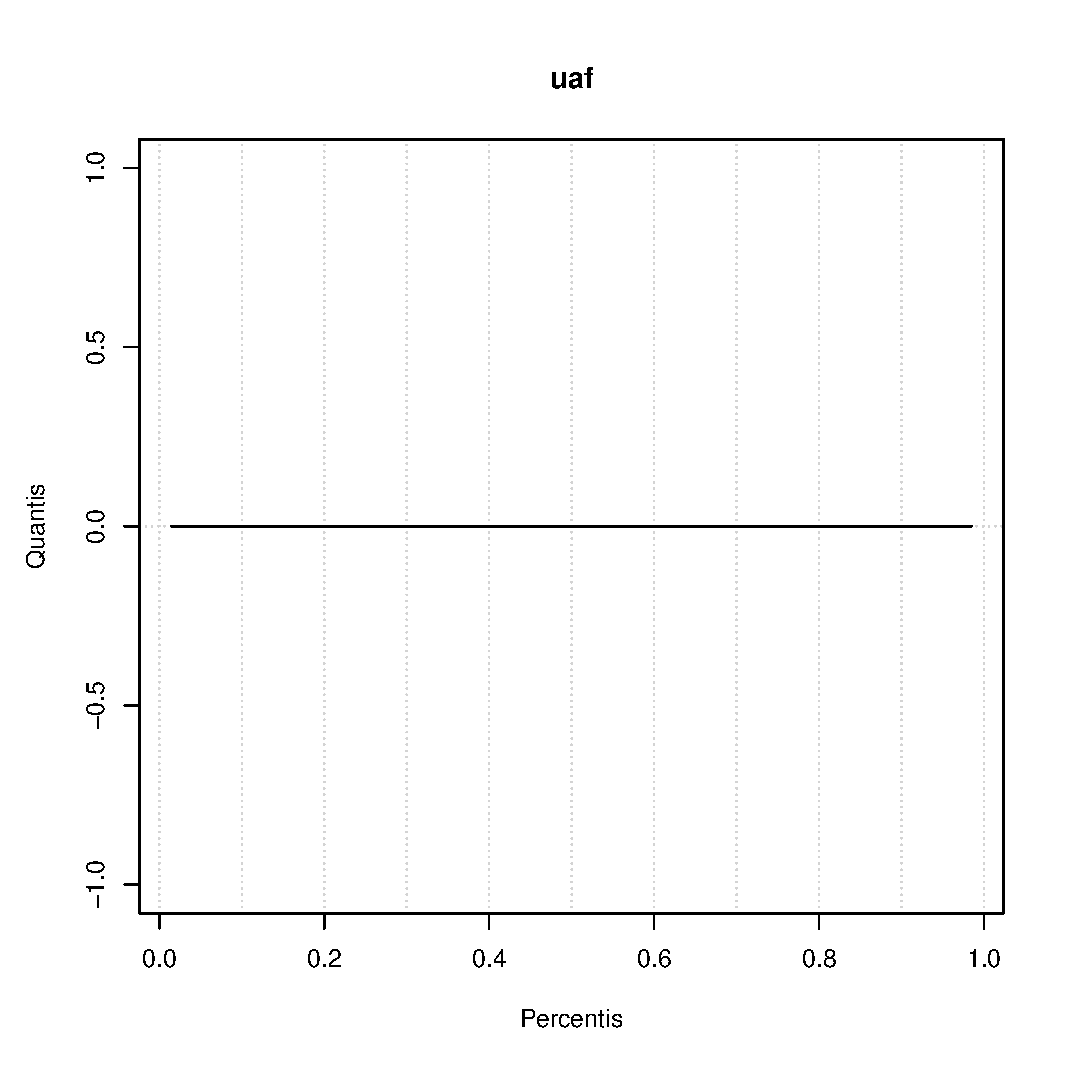
\includegraphics[width=0.6\textwidth]
      {dados/linux/uaf.eps}
  \caption{Gráfico de Percentis da métrica UAF}
\end{figure}

\begin{figure}[h]
  \centering
  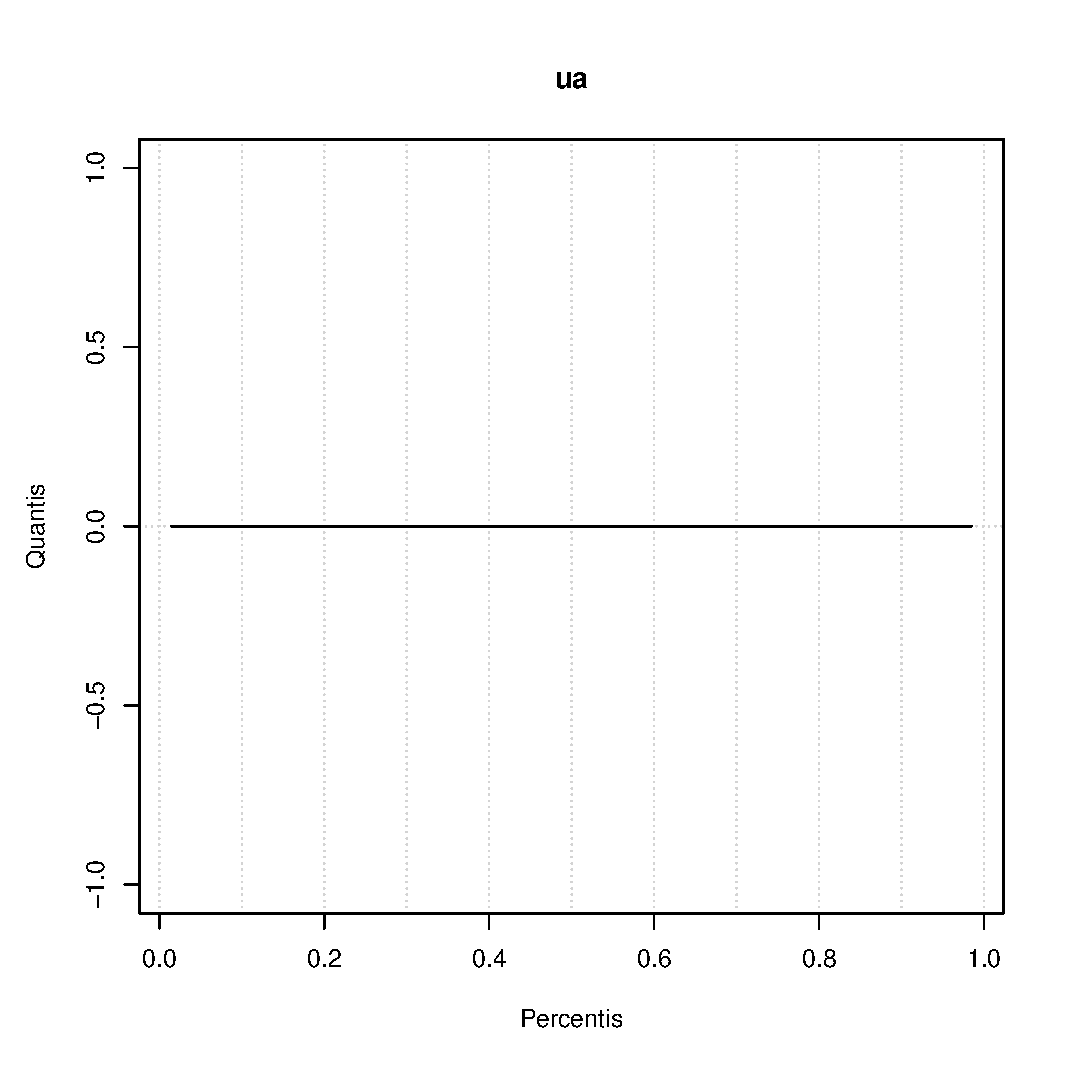
\includegraphics[width=0.6\textwidth]
      {dados/linux/ua.eps}
  \caption{Gráfico de Percentis da métrica UA}
\end{figure}

\newpage

\begin{figure}[h]
  \centering
  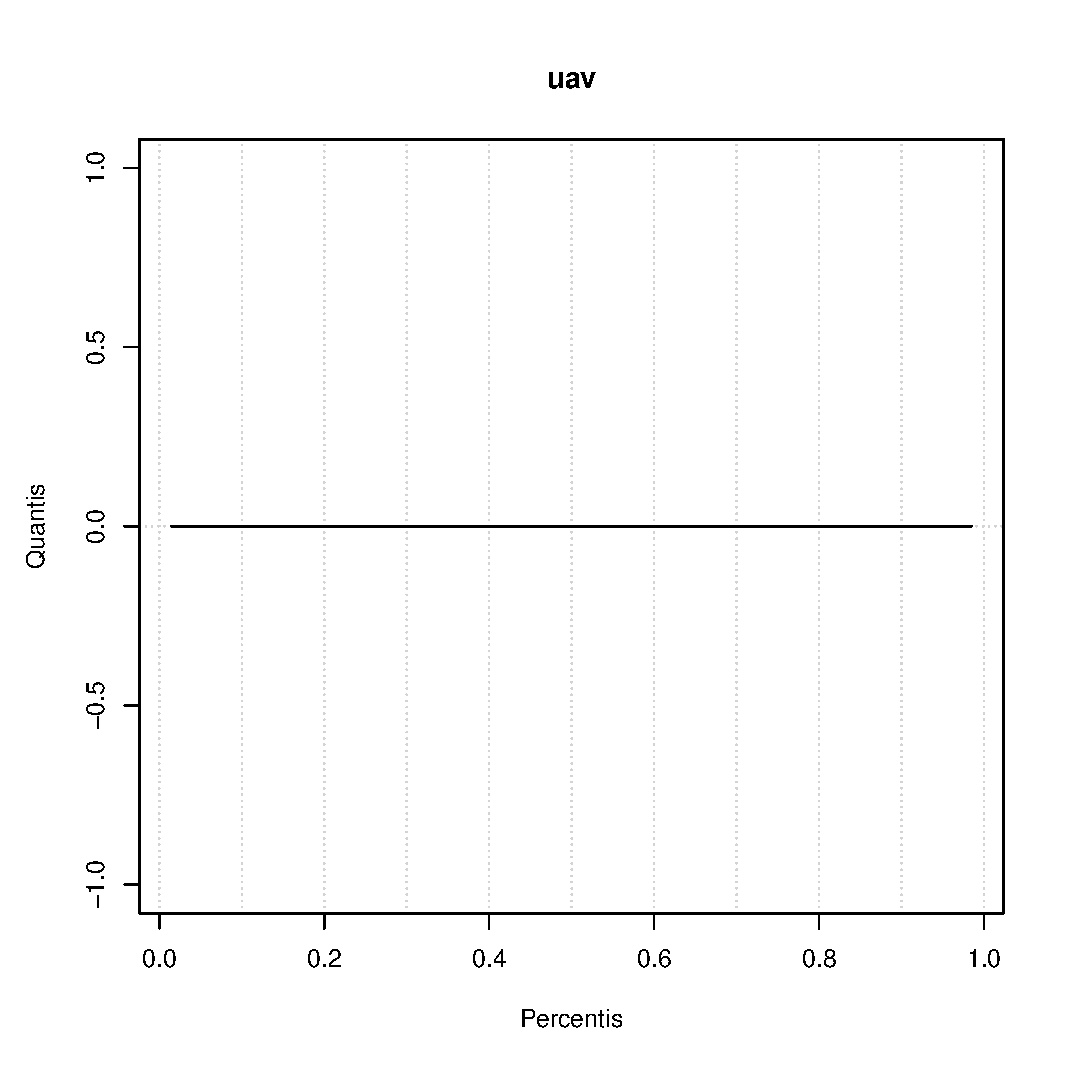
\includegraphics[width=0.6\textwidth]
      {dados/linux/uav.eps}
  \caption{Gráfico de Percentis da métrica UAV}
\end{figure}



\chapter{Análise Qualitativa} \label{anex:analise_qualitativa}

Neste anexo possui as tabelas de análise das métricas de vulnerabilidade de código fonte por módulo
dos projetos utilizados para realização da análise qualitativa, na seção \ref{sec:analise_qualitativa}.


\begin{table}[h]
\resizebox{\textwidth}{!}{%
\begin{tabular}{ccc}
\hline
\textbf{Métrica} & \textbf{Nº total de Módulos vulneráveis} & \textbf{\% de Módulos vulneráveis} \\ \hline
\rowcolor[HTML]{EFEFEF} 
\textbf{AN}      & 11                                       & 4.3478                             \\ \hline
\textbf{AUV}     & 2                                        & 0.7905                             \\ \hline
\rowcolor[HTML]{EFEFEF} 
\textbf{DNP}     & 22                                       & 8.6956                             \\ \hline
\textbf{MLK}     & 1                                        & 0.3952                             \\ \hline
\textbf{ROGU}    & 3                                        & 1.1857                             \\ \hline
\rowcolor[HTML]{EFEFEF} 
\textbf{UA}      & 1                                        & 0.3952                             \\ \hline
\textbf{UAV}     & 3                                        & 1.1857                             \\ \hline
\end{tabular}
}
\caption{Projeto Bash}
\end{table}



\begin{table}[h]
\resizebox{\textwidth}{!}{%
\begin{tabular}{ccc}
\hline
\textbf{Métrica} & \textbf{Nº total de Módulos vulneráveis} & \textbf{\% de Módulos vulneráveis} \\ \hline
\rowcolor[HTML]{EFEFEF} 
\textbf{AN}      & 7                                        & 0.4755                             \\ \hline
\textbf{AUV}     & 9                                        & 0.6114                             \\ \hline
\rowcolor[HTML]{EFEFEF} 
\textbf{DNP}     & 93                                       & 6.3179                             \\ \hline
\textbf{DUPV}    & 1                                        & 0.0679                             \\ \hline
\textbf{ROGU}    & 11                                       & 0.0563                             \\ \hline
\end{tabular}
}
\caption{Projeto Blender}
\end{table}





\begin{table}[h]
\resizebox{\textwidth}{!}{%
\begin{tabular}{ccc}
\hline
\textbf{Métrica} & \textbf{Nº total de Módulos vulneráveis} & \textbf{\% de Módulos vulneráveis} \\ \hline
\rowcolor[HTML]{EFEFEF} 
\textbf{AN}      & 10                                       & 0.5630                             \\ \hline
\textbf{AUV}     & 31                                       & 1.7454                             \\ \hline
\rowcolor[HTML]{EFEFEF} 
\textbf{DNP}     & 37                                       & 2.0833                             \\ \hline
\textbf{DUPV}    & 4                                        & 0.2252                             \\ \hline
\textbf{MLK}     & 1                                        & 0.0563                             \\ \hline
\rowcolor[HTML]{EFEFEF} 
\textbf{ROGU}    & 24                                       & 1.3513                             \\ \hline
\textbf{UAV}     & 13                                       & 1.1857                             \\ \hline
\end{tabular}
}
\caption{Projeto FFmpeg}
\end{table}




\begin{table}[h]
\resizebox{\textwidth}{!}{%
\begin{tabular}{ccc}
\hline
\textbf{Métrica} & \textbf{Nº total de Módulos vulneráveis} & \textbf{\% de Módulos vulneráveis} \\ \hline
\rowcolor[HTML]{EFEFEF} 
\textbf{AN}      & 29                                       & 0.2337                             \\ \hline
\textbf{ASOM}    & 7                                        & 0.0564                             \\ \hline
\rowcolor[HTML]{EFEFEF} 
\textbf{AUV}     & 24                                       & 0.1934                             \\ \hline
\textbf{DNP}     & 218                                      & 1.7574                             \\ \hline
\textbf{DUPV}    & 10                                       & 0.0806                             \\ \hline
\rowcolor[HTML]{EFEFEF} 
\textbf{MLK}     & 12                                       & 0.0967                             \\ \hline
\textbf{OBAA}    & 5                                        & 0.0403                             \\ \hline
\rowcolor[HTML]{EFEFEF} 
\textbf{ROGU}    & 34                                       & 0.2741                             \\ \hline
\textbf{SAIGV}   & 2                                        & 0.0161                             \\ \hline
\rowcolor[HTML]{EFEFEF} 
\textbf{UA}      & 6                                        & 0.0483                             \\ \hline
\textbf{UAF}     & 8                                        & 0.0644                             \\ \hline
\rowcolor[HTML]{EFEFEF} 
\textbf{UAV}     & 22                                       &                                    \\ \hline
\end{tabular}
}
\caption{Projeto Firefox}
\end{table}



\begin{table}[h]
\resizebox{\textwidth}{!}{%
\begin{tabular}{ccc}
\hline
\textbf{Métrica} & \textbf{Nº total de Módulos vulneráveis} & \textbf{\% de Módulos vulneráveis} \\ \hline
\rowcolor[HTML]{EFEFEF} 
\textbf{AN}      & 2                                        & 0.7575                             \\ \hline
\textbf{DNP}     & 16                                       & 6.0606                             \\ \hline
\rowcolor[HTML]{EFEFEF} 
\textbf{ROGU}    & 2                                        & 0.7575                             \\ \hline
\textbf{UAV}     & 4                                        & 1.5151                             \\ \hline
\end{tabular}
}
\caption{Projeto Gstreamer}
\end{table}




\begin{table}[h]
\resizebox{\textwidth}{!}{%
\begin{tabular}{ccc}
\hline
\textbf{Métrica} & \textbf{Nº total de Módulos vulneráveis} & \textbf{\% de Módulos vulneráveis} \\ \hline
\rowcolor[HTML]{EFEFEF} 
\textbf{AN}      & 3                                        & 0.1164                             \\ \hline
\textbf{AUV}     & 3                                        & 0.1164                             \\ \hline
\rowcolor[HTML]{EFEFEF} 
\textbf{DF}      & 1                                        & 0.0388                             \\ \hline
\textbf{DNP}     & 6                                        & 0.2329                             \\ \hline
\rowcolor[HTML]{EFEFEF} 
\textbf{MLK}     & 9                                        & 0.3493                             \\ \hline
\textbf{ROGU}    & 7                                        & 0.2717                             \\ \hline
\rowcolor[HTML]{EFEFEF} 
\textbf{SAIGV}   & 1                                        & 0.0388                             \\ \hline
\textbf{UA}      & 2                                        & 0.0776                             \\ \hline
\rowcolor[HTML]{EFEFEF} 
\textbf{UAF}     & 5                                        & 0.1940                             \\ \hline
\textbf{UAV}     & 3                                        & 3.2667                             \\ \hline
\end{tabular}
}
\caption{Projeto Inetutils}
\end{table}



\begin{table}[h]
\resizebox{\textwidth}{!}{%
\begin{tabular}{ccc}
\hline
\textbf{Métrica} & \textbf{Nº total de Módulos vulneráveis} & \textbf{\% de Módulos vulneráveis} \\ \hline
\rowcolor[HTML]{EFEFEF} 
\textbf{DNP}     & 40                                       & 0.1734                             \\ \hline
\textbf{DUPV}    & 3                                        & 0.0130                             \\ \hline
\rowcolor[HTML]{EFEFEF} 
\textbf{SAIGV}   & 1                                        & 0.0043                             \\ \hline
\end{tabular}
}
\caption{Projeto Linux Kernel}
\end{table}



\begin{table}[h]
\resizebox{\textwidth}{!}{%
\begin{tabular}{ccc}
\hline
\textbf{Métrica} & \textbf{Nº total de Módulos vulneráveis} & \textbf{\% de Módulos vulneráveis} \\ \hline
\rowcolor[HTML]{EFEFEF} 
\textbf{AN}      & 2                                        & 0.8064                             \\ \hline
\textbf{DNP}     & 7                                        & 2.8225                             \\ \hline
\rowcolor[HTML]{EFEFEF} 
\textbf{MLK}     & 2                                        & 0.8064                             \\ \hline
\textbf{UA}      & 1                                        & 0.4032                             \\ \hline
\textbf{UAF}     & 4                                        & 0.1026                             \\ \hline
\end{tabular}
}
\caption{Projeto OpenSSH}
\end{table}





\begin{table}[h]
\resizebox{\textwidth}{!}{%
\begin{tabular}{ccc}
\hline
\textbf{Métrica} & \textbf{Nº total de Módulos vulneráveis} & \textbf{\% de Módulos vulneráveis} \\ \hline
\rowcolor[HTML]{EFEFEF} 
\textbf{AN}      & 6                                        & 0.6160                             \\ \hline
\textbf{AUV}     & 1                                        & 0.1026                             \\ \hline
\rowcolor[HTML]{EFEFEF} 
\textbf{DNP}     & 14                                       & 1.4373                             \\ \hline
\textbf{ROGU}    & 6                                        & 0.6160                             \\ \hline
\textbf{UAV}     & 1                                        & 0.7472                             \\ \hline
\end{tabular}
}
\caption{Projeto OpenSSL}
\end{table}





\begin{table}[h]
\resizebox{\textwidth}{!}{%
\begin{tabular}{ccc}
\hline
\textbf{Métrica} & \textbf{Nº total de Módulos vulneráveis} & \textbf{\% de Módulos vulneráveis} \\ \hline
\rowcolor[HTML]{EFEFEF} 
\textbf{AN}      & 2                                        & 0.3629                             \\ \hline
\textbf{AUV}     & 4                                        & 0.7259                             \\ \hline
\rowcolor[HTML]{EFEFEF} 
\textbf{BF}      & 1                                        & 0.1814                             \\ \hline
\textbf{DNP}     & 18                                       & 3.2667                             \\ \hline
\rowcolor[HTML]{EFEFEF} 
\textbf{DUPV}    & 2                                        & 0.3629                             \\ \hline
\textbf{MLK}     & 2                                        & 0.3629                             \\ \hline
\rowcolor[HTML]{EFEFEF} 
\textbf{OBAA}    & 2                                        & 0.3629                             \\ \hline
\textbf{ROGU}    & 6                                        & 1.0889                             \\ \hline
\rowcolor[HTML]{EFEFEF} 
\textbf{UA}      & 1                                        & 0.1814                             \\ \hline
\textbf{UAV}     & 1                                        & 0.1164                             \\ \hline
\end{tabular}
}
\caption{Projeto Python2.7}
\end{table}




\begin{table}[h]
\resizebox{\textwidth}{!}{%
\begin{tabular}{ccc}
\hline
\textbf{Métrica} & \textbf{Nº total de Módulos vulneráveis} & \textbf{\% de Módulos vulneráveis} \\ \hline
\rowcolor[HTML]{EFEFEF} 
\textbf{AN}      & 4                                        & 1.0498                             \\ \hline
\textbf{ASOM}    & 2                                        & 0.5249                             \\ \hline
\rowcolor[HTML]{EFEFEF} 
\textbf{AUV}     & 2                                        & 0.5249                             \\ \hline
\textbf{DNP}     & 10                                       & 2.6246                             \\ \hline
\textbf{MLK}     & 1                                        & 0.2624                             \\ \hline
\rowcolor[HTML]{EFEFEF} 
\textbf{ROGU}    & 2                                        & 0.5249                             \\ \hline
\textbf{SAIGV}   & 1                                        & 0.2624                             \\ \hline
\rowcolor[HTML]{EFEFEF} 
\textbf{UAF}     & 1                                        & 0.2624                             \\ \hline
\textbf{UAV}     & 1                                        & 0.1814                             \\ \hline
\end{tabular}
}
\caption{Projeto Ruby-2.1}
\end{table}


\end{anexosenv}


%index:
  %\addtoindex{vulnerabilidade}
\addtoindex{fraqueza}
\addtoindex{bug}
\addtoindex{CWE}
\addtoindex{CVE}
\addtoindex{NIST}
\addtoindex{análise}
\addtoindex{avaliação}
\addtoindex{código}

  %\printindex

\end{document}

